%%%%%%%%%%%%%%%%%%%%%%%%%%%%%%%%%%%%%%%%%
% Structured General Purpose Assignment
% LaTeX Template
%
% This template has been downloaded from:
% http://www.latextemplates.com
%
% Original author:
% Ted Pavlic (http://www.tedpavlic.com)
%
% Note:
% The \lipsum[#] commands throughout this template generate dummy text
% to fill the template out. These commands should all be removed when 
% writing assignment content.
%
%%%%%%%%%%%%%%%%%%%%%%%%%%%%%%%%%%%%%%%%%

%----------------------------------------------------------------------------------------
%	PACKAGES AND OTHER DOCUMENT CONFIGURATIONS
%----------------------------------------------------------------------------------------
\documentclass{Askarticle}
\usepackage[utf8]{inputenc}
\usepackage{fancyhdr} % Required for custom headers
\usepackage{lastpage} % Required to determine the last page for the footer
\usepackage{extramarks} % Required for headers and footers
\usepackage{graphicx} % Required to insert images
\usepackage{lipsum} % Used for inserting dummy 'Lorem ipsum' text into the template
\usepackage{amsmath}
\usepackage{amsfonts}
\usepackage{listings}
\usepackage{color}
%\usepackage{slashbox}
\usepackage{verbatim}
\usepackage{graphicx}
\usepackage{subfig}% http://ctan.org/pkg/subfig
\usepackage[breakwords]{truncate}

\usepackage{fancybox}
\usepackage{tikz}
\usepackage{array}
\usepackage{multirow}

 \usepackage[utf8]{inputenc}
\usepackage[english]{babel}

 
\usepackage{amsthm}
 
\usepackage[colorinlistoftodos]{todonotes}
\usepackage{algorithm}
\usepackage{algpseudocode}

\usepackage{color} %for colored boxes
\usepackage{empheq}

\usepackage{listings} %to include Code
\usepackage{booktabs} %for tables


%%CONFUSION MATRIX%%
\newcommand\MyBox[2]{
  \fbox{\lower0.75cm
    \vbox to 1.0cm{\vfil
      \hbox to 1.2cm{\hfil\parbox{0.4cm}{#1}\hfil}
      \vfil}%
  }%
}


\usepackage{geometry}
 \geometry{
 a4paper,
 total={210mm,297mm},
 left=20mm,
 right=20mm,
 top=20mm,
 bottom=20mm,
 }

%---------------------------------------------------------------------------------------------
%LISTINGS INITIAL
%---------------------------------------------------------------------------------------------
\definecolor{codegreen}{rgb}{0,0.6,0}
\definecolor{codegray}{rgb}{0.5,0.5,0.5}
\definecolor{codepurple}{rgb}{0.58,0,0.82}
\definecolor{backcolour}{rgb}{0.95,0.95,0.92}
 
\lstdefinestyle{mystyle}{
    backgroundcolor=\color{backcolour},   
    commentstyle=\color{codegreen},
    keywordstyle=\color{magenta},
    numberstyle=\tiny\color{codegray},
    stringstyle=\color{codepurple},
    basicstyle={\ttfamily \footnotesize},
    breakatwhitespace=false,         
    breaklines=true,                 
    captionpos=b,                    
    keepspaces=true,                 
    numbers=left,                    
    numbersep=5pt,                  
    showspaces=false,                
    showstringspaces=false,
    showtabs=false,                  
    tabsize=2
}
 
\lstset{style=mystyle}
%---------------------------------------------------------------------------------------------
% Margins
\topmargin=-0.45in
\evensidemargin=0in
\oddsidemargin=0in
\textwidth=6.5in
\textheight=9.0in
\headsep=0.25in 

\linespread{1.1} % Line spacing

% Set up the header and footer
\pagestyle{fancy}
%\lhead{\hmwkAuthorName} % Top left header
\rhead{\hmwkClass\ : \hmwkTitle} % Top center header
%\chead{\firstxmark} % Top right header
%\lfoot{\truncate{14cm}{\lastxmark}} % Bottom left footer
\cfoot{} % Bottom center footer
\rfoot{Page\ \thepage\ of\ \pageref{LastPage}} % Bottom right footer
\renewcommand\headrulewidth{0.4pt} % Size of the header rule
\renewcommand\footrulewidth{0.4pt} % Size of the footer rule

\setlength\parindent{0pt} % Removes all indentation from paragraphs

%----------------------------------------------------------------------------------------
%	DOCUMENT STRUCTURE COMMANDS
%	Skip this unless you know what you're doing
%----------------------------------------------------------------------------------------

% Header and footer for when a page split occurs within a problem environment
\newcommand{\enterProblemHeader}[1]{
\nobreak\extramarks{#1}{#1 continued on next page\ldots}\nobreak
\nobreak\extramarks{#1 (continued)}{#1 continued on next page\ldots}\nobreak
}

% Header and footer for when a page split occurs between problem environments
\newcommand{\exitProblemHeader}[1]{
\nobreak\extramarks{#1 (continued)}{#1 continued on next page\ldots}\nobreak
\nobreak\extramarks{#1}{}\nobreak
}

\setcounter{secnumdepth}{0} % Removes default section numbers
\newcounter{homeworkProblemCounter} % Creates a counter to keep track of the number of problems

\newcommand{\homeworkProblemName}{}
\newenvironment{homeworkProblem}[1][Problem \arabic{homeworkProblemCounter}]{ % Makes a new environment called homeworkProblem which takes 1 argument (custom name) but the default is "Problem #"
\stepcounter{homeworkProblemCounter} % Increase counter for number of problems
\renewcommand{\homeworkProblemName}{#1} % Assign \homeworkProblemName the name of the problem
\section{\homeworkProblemName} % Make a section in the document with the custom problem count
\enterProblemHeader{\homeworkProblemName} % Header and footer within the environment
}{
\exitProblemHeader{\homeworkProblemName} % Header and footer after the environment
}

\newcommand{\problemAnswer}[1]{ % Defines the problem answer command with the content as the only argument
\noindent\framebox[\columnwidth][c]{\begin{minipage}{0.98\columnwidth}#1\end{minipage}} % Makes the box around the problem answer and puts the content inside
}

\newcommand{\homeworkSectionName}{}
\newenvironment{homeworkSection}[1]{ % New environment for sections within homework problems, takes 1 argument - the name of the section
\renewcommand{\homeworkSectionName}{#1} % Assign \homeworkSectionName to the name of the section from the environment argument
\subsection{\homeworkSectionName} % Make a subsection with the custom name of the subsection
\enterProblemHeader{\homeworkProblemName\ [\homeworkSectionName]} % Header and footer within the environment
}{
\enterProblemHeader{\homeworkProblemName} % Header and footer after the environment
}
   
%----------------------------------------------------------------------------------------
%	NAME AND CLASS SECTION
%----------------------------------------------------------------------------------------
\newcommand\given[1][]{\:#1\vert\:} %define new command
\newcommand{\hmwkTitle}{Final} % Assignment title
\newcommand{\hmwkDueDate}{\today} % Due date
\newcommand{\hmwkClass}{TIM\ 245 - Data Mining} % Course/class
\newcommand{\hmwkClassTime}{4:20pm} % Class/lecture time
\newcommand{\hmwkClassInstructor}{Instructor: Tyler Munger} % Teacher/lecturer
\newcommand{\hmwkAuthorNameB}{Panos Karagiannis}
\newcommand{\hmwkOption}{Homework Heavy Option}
\newcommand{\hmwkIDA}{ID: -}

\newcommand{\Prb}{\mathbb{P}}
\newcommand{\N}{\mathcal{N}}
\newcommand{\R}{\mathbb{R}}
\newcommand{\E}{\mathbb{E}}
\newcommand{\answer}{\noindent\rule{16cm}{0.9pt}
		
		\large{\textbf{\underline{Answer:}}}

		\vspace{0.5cm}}
%----------------------------------------------------------------------------------------
%	TITLE PAGE
%----------------------------------------------------------------------------------------

\title{
\vspace{2in}
\textmd{\textbf{\hmwkClass:\ \hmwkTitle}}\\
\normalsize\vspace{0.1in}\small{Due:\ \textit{\hmwkDueDate}}\\
\vspace{0.1in}\large{\textit{\hmwkClassInstructor}}
\vspace{3in}
}

\author{\begin{tabular}{ l r }
					 \hmwkAuthorNameB \\
					\multicolumn{1}{c}{\hmwkIDA}
				\end{tabular}}
\date{} % Insert date here if you want it to appear below your name

%----------------------------------------------------------------------------------------

\begin{document}

\maketitle

%----------------------------------------------------------------------------------------
%	TABLE OF CONTENTS
%----------------------------------------------------------------------------------------

%\setcounter{tocdepth}{1} % Uncomment this line if you don't want subsections listed in the ToC

\newpage
\tableofcontents
\newpage

\newtheorem{theorem}{Theorem}
\newtheorem{panostheorem}{Theorem}
\newtheorem{claim}[theorem]{Claim}
\newtheorem{definition}[panostheorem]{Definition}

%----------------------------------------------------------------------------------------
%	BLUE BOX
%----------------------------------------------------------------------------------------



\definecolor{myblue}{rgb}{.8, .8, 1}



\newlength\mytemplen
\newsavebox\mytempbox

\makeatletter
\newcommand\mybluebox{%
    \@ifnextchar[%]
       {\@mybluebox}%
       {\@mybluebox[0pt]}}

\def\@mybluebox[#1]{%
    \@ifnextchar[%]
       {\@@mybluebox[#1]}%
       {\@@mybluebox[#1][0pt]}}

\def\@@mybluebox[#1][#2]#3{
    \sbox\mytempbox{#3}%
    \mytemplen\ht\mytempbox
    \advance\mytemplen #1\relax
    \ht\mytempbox\mytemplen
    \mytemplen\dp\mytempbox
    \advance\mytemplen #2\relax
    \dp\mytempbox\mytemplen
    \colorbox{myblue}{\hspace{1em}\usebox{\mytempbox}\hspace{1em}}}
    

\makeatother




%----------------------------------------------------------------------------------------
%	PROBLEM 1
%----------------------------------------------------------------------------------------

\begin{homeworkProblem}[Problem \arabic{homeworkProblemCounter}: Classification Problem for Venture Capital Investment (30 points)  ]
The firm has assembled a dataset of the historical investments that includes both the initial assessment of the company and final the investment rating (Green, Yellow, Red). You have been asked to perform the following tasks related to creating a classification model that be used to determine if a new company is likely to be a Green, Yellow, or Red investment based on their assessment.


\begin{enumerate}
\item	Perform your EDA process, developed during your work at Xenefits, on the investment dataset and format the results into a well-structured report. Perform any data pre-processing steps (cleaning, transformation, etc.) necessary for addressing data quality issues that were discovered during the EDA process.
\item	Before you start, the firm would like a written statement of your process for creating the classification model. (Hint: The process might include the steps such as experimenting with different learning algorithms or model evaluation).
\item	Next, apply your process to create the classification model.
\item	Based on your process, what is the best classification model for predicting an investment rating? What is your assessment of this classification model? Is the performance good enough for the firm to use when making investment decisions?
What are some of the issues associated with equally weighting misclassification across the three classes (hint: is a Red misclassified as a Green the same as a Yellow misclassified as a Green?). Describe one possible solution for addressing this problem

\end{enumerate}

\textbf{Extra Credit}:\\
 Implement your solution for addressing the misclassification problem. Compare and contrast the results.


%In addition, we will explore whether the dataset contains any \textbf{missing values} and we will also suggest a way of \textbf{handling them}.
%We define outliers to be data points that are significantly far from the central tendency and we adopt a Parametric Outlier Analysis where we select a quantile cutoff for outliers.
\noindent\rule{16cm}{0.9pt}
		
\large{\textbf{\underline{Answer:}}}

\begin{enumerate}
\item Real world data are often \textbf{Incomplete}, \textbf{Noisy} as well as \textbf{Inconsistent}. Our \emph{Exploratory Data Analysis} (EDA) consists of a combination of \textbf{visual} and \textbf{quantitative} tools to answer important questions for each selected attribute in our dataset. More precisely, since every attribute is categorical we will look into descriptive statistics such as the \textbf{mode} and the \textbf{frequency}. Moreover, we will employ visual tools in order to determine whether a particular distribution is \textbf{unimodal}, \textbf{bimodal} or \textbf{multimodal}. \\

By looking at Table \ref{tbl:tables} we see that there is large variety of combinations of \emph{missing, low, medium} and \emph{high} values. More precisely, we observe attributes that have more \emph{missing} than actual values (ex. \texttt{INO, EFF, PPL}), and we expect this fact to undermine the quality of our classification algorithms. Moreover, the majority of the distributions are \emph{bimodal} or \emph{multimodal} with very few \emph{unimodal} ones. We expect to face difficulties in learning very skewed distributions correctly, since there will be insufficient data to train (i.e. \texttt{GRO} has only $1$ \emph{high} value). Finally, in the \texttt{rating} attribute, we see that the majority of values are \texttt{red}, followed by \texttt{green} and \texttt{yellow}. \\

In order to use the data in our classification models, we first encode all the categorical variables as numerical. More precisely, since each attribute has $3$ values (ignoring missing), we create $3$ new \textbf{binary} variables for each attribute. \\

Initially, we thought of deleting the \textbf{missing} values, in order to perform classification but that yielded a dataset with only $8$ instances, clearly insufficient to perform learning. Instead, we replace the missing values of a given attribute with the \textbf{mode} value for this attribute. \\

Lastly, since our dataset consists of values between 0 and 1 we do not need to \textbf{normalize} the data or remove \textbf{outliers}. Also, the dataset does not contain any \textbf{inconsistencies}. 


\item At this stage, we will experiment with various classification models in order to determine which one yields the best results. First we will create a baseline model, which will be very simple and interpretable and is going to provide us with a benchmark to compare the rest of our models. In order to evaluate our models we will consider two metrics, namely, \textbf{accuracy} and \textbf{F-measure}. \\

The baseline model that we use, is the \textbf{ZeroR} model, whereas, the more elaborate models that we consider are: \textbf{SVM, Logistic Regression, KNN}. \\

In terms of \textbf{complexity},  \emph{SVM and Logistic Regression} models, behave very similarly in this problem. These models minimize a convex loss functions and hence any local minimum is also guaranteed to be a global minimum as well. As far as $KNN$ is concerned, it does not minimize a loss function, yet, the computation of the ``distance'' between data points can be very expensive if many features are incorporated into the model. \\

\textbf{It has to be mentioned}, that all these models have similar complexities for relatively small number of attributes, as it is in the case of $Xenefits$. \textbf{Nevertheless}, if the management wanted to incorporate more attributes into the model then the complexities of \emph{Logistic Regression and KNN} would explode, whereas, \emph{SVM} can tackle this problem. In  \emph{SVM}, we can proceed by solving the \emph{Dual problem } instead of the \emph{Primal} and using a \emph{Kernel function} to retrieve the weights (a detailed explanation of this fact was submitted in HW2 when comparing Logistic Regression and SVM). \\

As far as \textbf{performance} is concerned, $KNN$ tend to overfit the data more easily than the other two methods. Therefore, in a $KNN$ model we should carefully decide on the parameter $K$. Similarly in an \emph{SVM} model as we increase the parameter $C$ we decrease the tolerance for misclassification but if we increase too much there is the danger of overfitting the data ($C\gg0$ is like a hard margin). Also, \emph{Logistic Regression} models can overfit but we can control the size of the coefficient of the model by introducing regularization.  \\


Finally, in terms of \textbf{interpretability} the simplest model is $KNN$ since no function minimization is involved. \emph{SVM and Logistic Regression} are more complex models which try to maximize the \emph{margin} and model the class conditional probabilities, respectively. \emph{ Logistic Regression} is always non-linear, whereas, in \emph{SVM} a non-linear Kernel function is frequently used. In the following parts we use the \textbf{Normalized Polynomial Kernel} for our \emph{SVM}  model.

\item In Table \ref{table:res} we see the performance of the aforementioned models:
\begin{table}[H]
		\caption{Performance of classification models for determining the \texttt{rating}. R., Y., G. stand for Red, Yellow, Green, respectively}
		\centering
		\begin{tabular}{c c c c c c}
		\hline\hline
		{} & Accuracy(\%) & F-measure R. &F-measure Y. &F-measure G.  & Weighted F-measure  \\ [0.5ex] % inserts table %heading
		\hline
		SVM (C=1)& 89.21 & 0.94 & 0.73 & 0.87 & \textbf{0.89} \\  
		Logistic Regression &76.47 & 0.86 & 0.55 & 0.71 & 0.77  \\
		KNN (K=1) & 86.27 & 0.9  & 0.75 & 0.86 & 0.87  \\
		ZeroR & 52.94 & 0.69 & 0 & 0  & 0.37 \\
		%\\ [1ex]
		\hline
		\end{tabular}\\[0.5cm]
		\label{table:res}
\end{table}

\item Simply by looking at the above table, we see that the more elaborate models outperform the baseline (\emph{ZeroR}) both in terms of accuracy and F-measure. We see that the best performing model is \textbf{SVM} with \textbf{KNN} performing similarly. \\

Nevertheless, we need to be particularly careful with the assessment metrics we use. Since there are large class imbalances ($53\%$ red, $ 29\%$ yellow, $18\%$ green), the accuracy metric is not very useful because many models learn to predict the majority of class most of the times. Instead, to obtain a better evaluation, we look at the confusion matrix (Table \ref{table:conf}) and the F-score computed in Table \ref{table:res}.
\begin{table}[H]
		\caption{Confusion matrix for SVM}
		\centering
\begin{tabular}{c >{\bfseries}r @{\hspace{0.9em}}c @{\hspace{0.9em}}c @{\hspace{0.9em}}l}
  \multirow{14}{*}{\parbox{1.9cm}{\bfseries\raggedleft Actual\\ Value}} & 
    & \multicolumn{2}{c}{\bfseries Classified as:} & \\
  & & \bfseries red & \bfseries yellow & \bfseries green \\
  & red & \MyBox{51}{Times} & \MyBox{1}{Time} & \MyBox{2}{Times} \\[2.4em]
  & yellow & \MyBox{2}{Times} & \MyBox{11}{Times} & \MyBox{5}{Times} \\ [2.4em]
  & green & \MyBox{1}{Time} & \MyBox{0}{Times} & \MyBox{29}{Times} \\
\end{tabular}
\label{table:conf}
\end{table}

By observing the confusion matrix, we see that the SVM model has managed to partially limit the effect of the unbalanced classes. Nevertheless, we observe that the model tends to misclassify \emph{yellow} much more that it tends to misclassify \emph{red}. More precisely, the \textbf{effect of the imbalances classes} is seen in the model, when it misclassifies $18\%(=5/18)$ of the yellow values whereas it only misclassifies $3\%= 2/54$ of the total red values.

Finally, since the company needs to make crucial investment decision, where many millions of dollars are involved, we would say that the results of the model are   \textbf{still not very good} to allow the company to be profitable. 

\item As explained in (4), one of the most important problems with class imbalances is that the model tends to predict the majority class more often than the other classes, and hence obtains a good accuracy score. For example, the accuracy of the $SVM$ model is $89\%$, nevertheless, by looking at the confusion matrix the model misclassifies $18\%(=5/18)$ of the yellow values.  A possible solution to that problem would be to \textbf{under-resample the  dataset}, by deleting instances from the over-represented classes. This approach is easy to implement and fast to run, hence, it constitutes a good starting point.
\end{enumerate}

\textbf{Extra Credit}: \\
In order to eliminate the problem created by the imbalanced classes, we randomly sample $40\%$ and $70\%$ of the initial red and green values, respectively. Thus, we are left with a total of $61$ instances out of which $22$ have red rating, $21$ have green rating and $18$ have yellow rating. \\

Applying an SVM model to our data we get: 
\begin{table}[H]
		\caption{Performance of the SVM model when trained on balanced classes}
		\centering
		\begin{tabular}{c c c c c c}
		\hline\hline
		{} & Accuracy(\%) & F-measure R. &F-measure Y. &F-measure G.  & Weighted F-measure  \\ [0.5ex] % inserts table %heading
		\hline
		SVM (C=1)& 82 & 0.87 &  0.79 & 0.80 & 0.82\\  
		%\\ [1ex]
		\hline
		\end{tabular}\\[0.5cm]
		\label{table:res_b}
\end{table}

\begin{table}[H]
		\caption{Confusion matrix for SVM}
		\centering
\begin{tabular}{c >{\bfseries}r @{\hspace{0.9em}}c @{\hspace{0.9em}}c @{\hspace{0.9em}}l}
  \multirow{14}{*}{\parbox{1.9cm}{\bfseries\raggedleft Actual\\ Value}} & 
    & \multicolumn{2}{c}{\bfseries Classified as:} & \\
  & & \bfseries red & \bfseries yellow & \bfseries green \\
  & red & \MyBox{17}{Times} & \MyBox{1}{Time} & \MyBox{5}{Times} \\[2.4em]
  & yellow & \MyBox{0}{Times} & \MyBox{13}{Times} & \MyBox{5}{Times} \\ [2.4em]
  & green & \MyBox{0}{Time} & \MyBox{1}{Times} & \MyBox{20}{Times} \\
\end{tabular}
\label{table:conf_b}
\end{table}

By looking at Table \ref{table:res_b} we see that the model performs worse than before in both accuracy and F-measure, but this can be attributed to the fact that we are now using $40\%$ less data to train our classifier. \\

What is important to observe, is that now the proportion of red ratings misclassified as green is $18\% (= 4/22)$, whereas the proportion of yellow ratings misclassified as green is $27\% (= 5/18)$. The difference now is \textbf{much smaller} than previously, since our classifier has learned to ``balance'' the classes.

\begin{center}
\textsc{ \textbf{Appendix for Problem 1} }
\end{center}


%%% TABLES %%%%
\begin{table}[H]%
  \centering
  \subfloat[][]{
  
\begin{tabular}{lr}
\toprule
 EFF &  count \\
\midrule
Missing      &     61 \\
low    &     40 \\
medium &      1 \\
\bottomrule
\end{tabular}

  }%
  \qquad
  \subfloat[][]{
\begin{tabular}{lr}
\toprule
GRO&  count \\
\midrule
high   &      1 \\
low    &     87 \\
medium &     14 \\
\bottomrule
\end{tabular}
  
  }
 \qquad
\subfloat[][]{


\begin{tabular}{lr}
\toprule
{MKT} &  count \\
\midrule
low    &     83 \\
medium &     19 \\
\bottomrule
\end{tabular}
  
  }
\qquad
\subfloat[][]{


\begin{tabular}{lr}
\toprule
{EXP} &  count \\
\midrule
low    &     94 \\
medium &      8 \\
\bottomrule
\end{tabular}
  
  } 
\qquad
\subfloat[][]{


\begin{tabular}{lr}
\toprule
{CPL} &  count \\
\midrule
high   &     20 \\
low    &     22 \\
medium &     60 \\
\bottomrule
\end{tabular}
  
  }
  \qquad
\subfloat[][]{


\begin{tabular}{lr}
\toprule
{INO} &  count \\
\midrule
Missing      &     59 \\
low    &     36 \\
medium &      7 \\
\bottomrule
\end{tabular}
  
  }
    \qquad
\subfloat[][]{



\begin{tabular}{lr}
\toprule
{TCH} &  count \\
\midrule
Missing      &     25 \\
low    &     50 \\
medium &     27 \\
\bottomrule
\end{tabular}
  
  }
      \qquad
\subfloat[][]{

\begin{tabular}{lr}
\toprule
{JNT} &  count \\
\midrule
low    &     96 \\
medium &      6 \\
\bottomrule
\end{tabular}
  
  }
        \qquad
\subfloat[][]{

\begin{tabular}{lr}
\toprule
{PTN} &  count \\
\midrule
low    &     74 \\
medium &     28 \\
\bottomrule
\end{tabular}
  
  }
          \qquad
\subfloat[][]{

\begin{tabular}{lr}
\toprule
{MAC} &  count \\
\midrule
high   &     35 \\
low    &     43 \\
medium &     24 \\
\bottomrule
\end{tabular}
  
  }
\qquad
\subfloat[][]{

\begin{tabular}{lr}
\toprule
{VPR} &  count \\
\midrule
high   &     30 \\
low    &     25 \\
medium &     47 \\
\bottomrule
\end{tabular}

  
  }
  \qquad
\subfloat[][]{

\begin{tabular}{lr}
\toprule
{PPL} &  count \\
 \midrule
Missing      &     31 \\
high   &      8 \\
low    &     34 \\
medium &     29 \\
\bottomrule
\end{tabular}

  
  }
\qquad
\subfloat[][]{

\begin{tabular}{lr}
\toprule
{SCH} &  count \\
\midrule
Missing      &     11 \\
high   &     40 \\
low    &     38 \\
medium &     13 \\
\bottomrule
\end{tabular}

  
  }
  \qquad
\subfloat[][]{


\begin{tabular}{lr}
\toprule
{PRT} &  count \\
 \midrule
high   &     59 \\
low    &     24 \\
medium &     19 \\
\bottomrule
\end{tabular}

  
  }
  \qquad
\subfloat[][]{


\begin{tabular}{lr}
\toprule
{MGR} &  count \\
\midrule
high   &     27 \\
low    &     29 \\
medium &     46 \\
\bottomrule
\end{tabular}

  
  }
    \qquad
\subfloat[][]{


\begin{tabular}{lr}
\toprule
{SOM} &  count \\
\midrule
Missing   &      6 \\
low &     96 \\
\bottomrule
\end{tabular}

  
  }
 \qquad
\subfloat[][]{


\begin{tabular}{lr}
\toprule
{MXS} &  count \\
\midrule
high   &     84 \\
low    &      7 \\
medium &     11 \\
\bottomrule
\end{tabular}
  
  }
   \qquad
\subfloat[][]{


\begin{tabular}{lr}
\toprule
{CMP} &  count \\
 \midrule
high   &     17 \\
low    &     66 \\
medium &     19 \\
\bottomrule
\end{tabular}
  
  }
   \qquad
\subfloat[][]{


\begin{tabular}{lr}
\toprule
{MDV} &  count \\
 \midrule
high   &     14 \\
low    &     65 \\
medium &     23 \\
\bottomrule
\end{tabular}
  
  }
     \qquad
\subfloat[][]{


\begin{tabular}{lr}
\toprule
{rating} &  count \\
\midrule
green  &     30 \\
red    &     54 \\
yellow &     18 \\
\bottomrule
\end{tabular}
}

  \caption{Frequency Tables for all attributes in the dataset.}%
  \label{tbl:tables}%
\end{table}





%%FIGURES%%
\begin{figure}[H]%
  \centering
  \subfloat[][]{
  
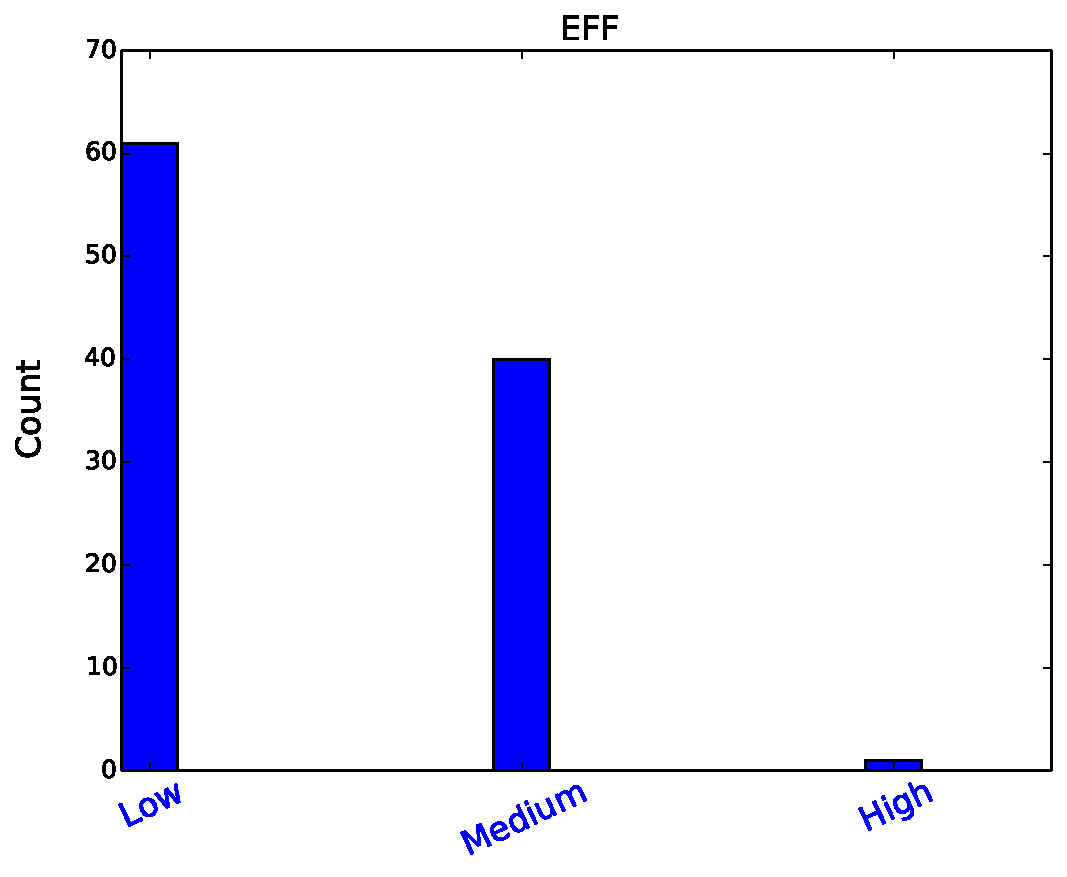
\includegraphics[width=0.29\textwidth]{../Code/ClassificationPlots/EFF_bar.pdf}\hfill

  }%
  \qquad
  \subfloat[][]{
  
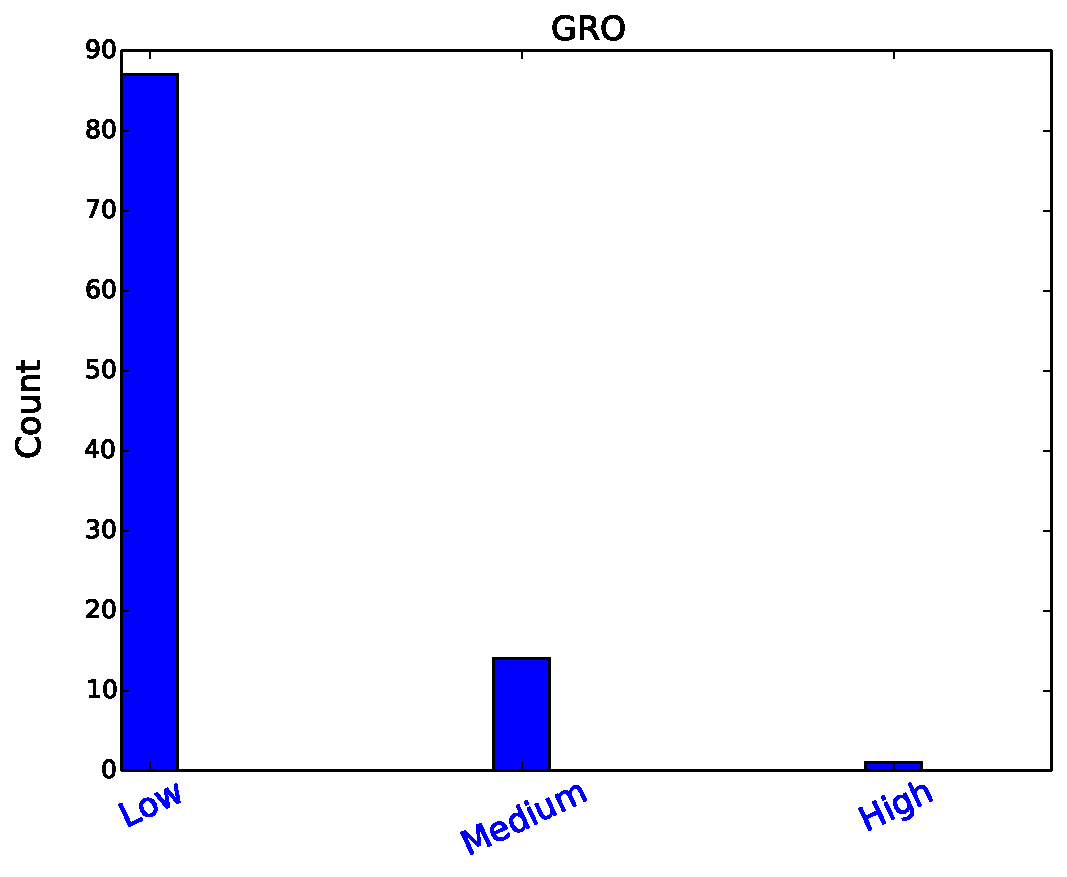
\includegraphics[width=0.29\textwidth]{../Code/ClassificationPlots/GRO_bar.pdf}\hfill
  
  }
 \qquad
\subfloat[][]{


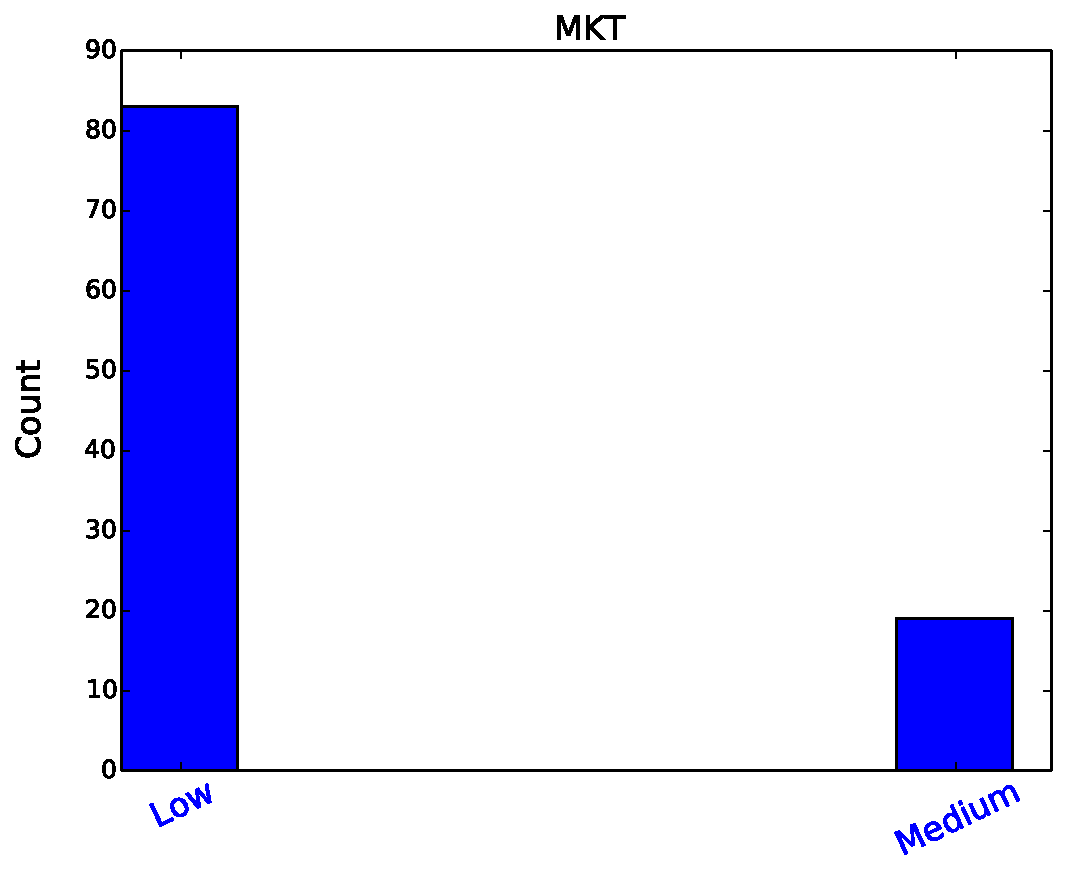
\includegraphics[width=0.29\textwidth]{../Code/ClassificationPlots/MKT_bar.pdf}\hfill
  
  }
\qquad
\subfloat[][]{


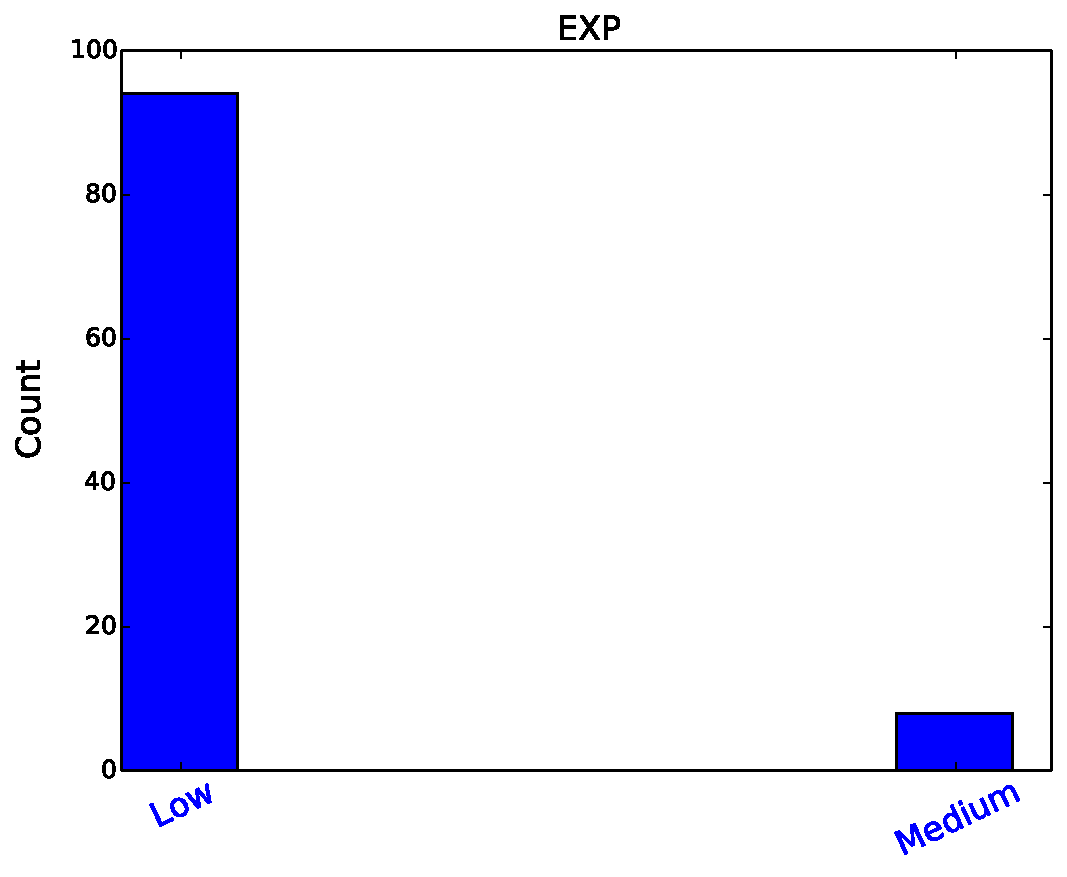
\includegraphics[width=0.29\textwidth]{../Code/ClassificationPlots/EXP_bar.pdf}\hfill
  
  } 
\qquad
\subfloat[][]{


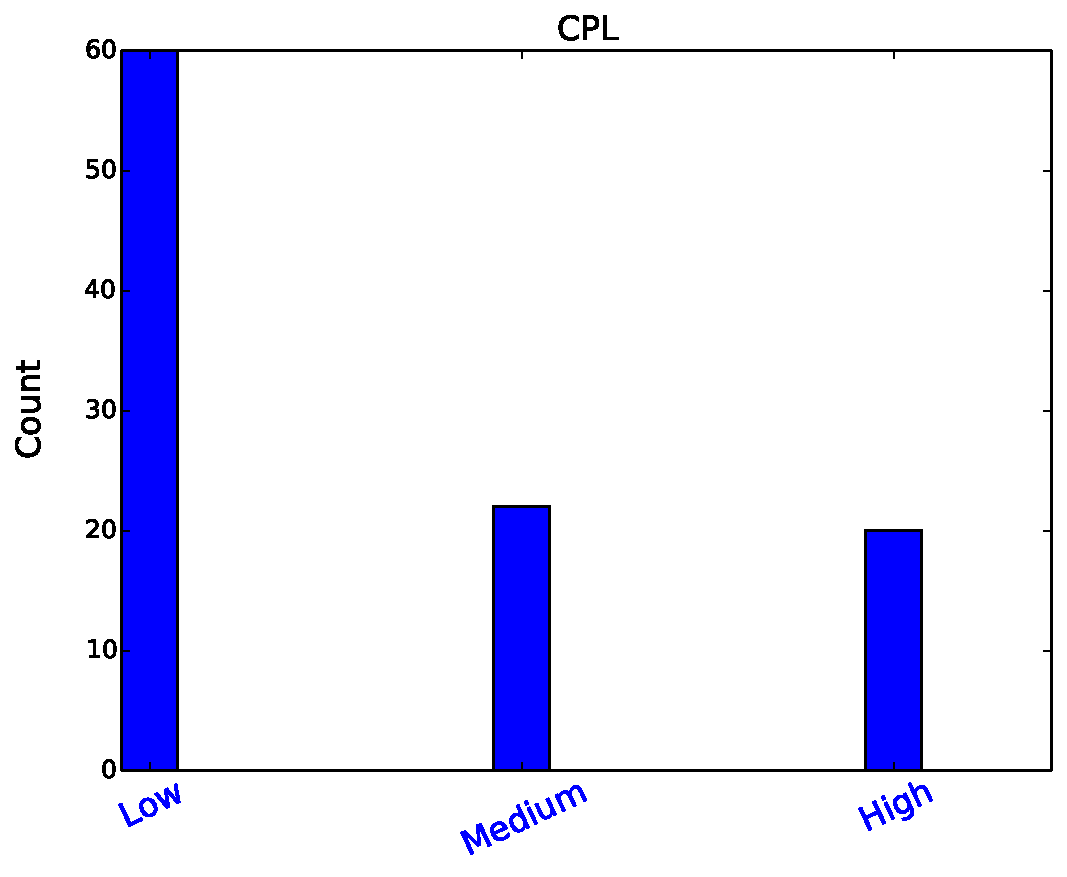
\includegraphics[width=0.29\textwidth]{../Code/ClassificationPlots/CPL_bar.pdf}\hfill
  
  }
  \qquad
\subfloat[][]{


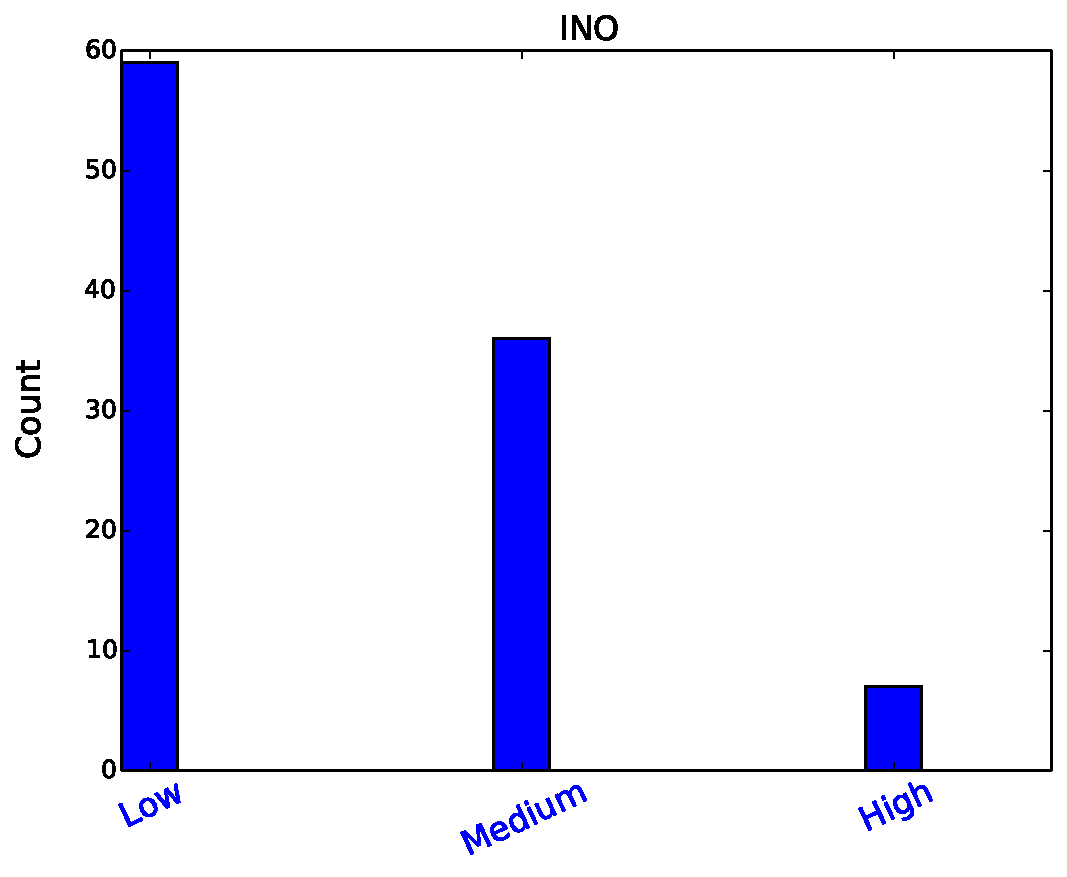
\includegraphics[width=0.29\textwidth]{../Code/ClassificationPlots/INO_bar.pdf}\hfill
  
  }
    \qquad
\subfloat[][]{



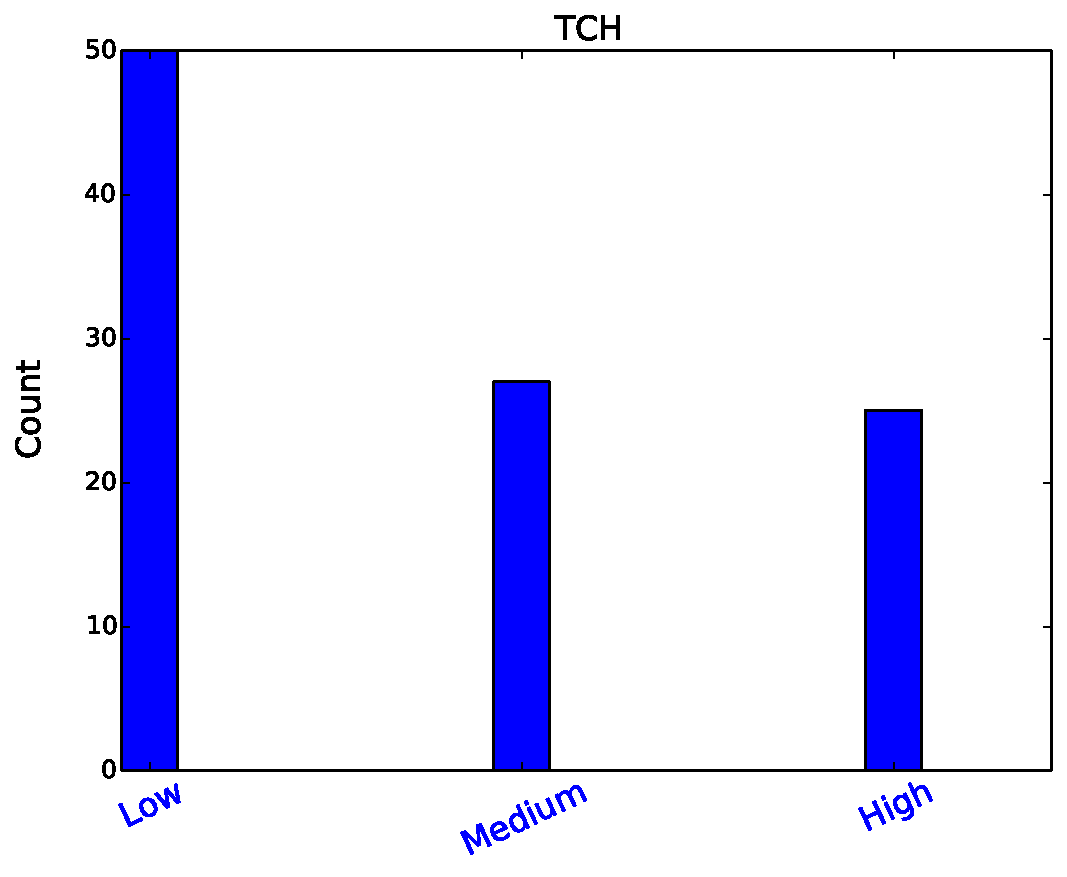
\includegraphics[width=0.29\textwidth]{../Code/ClassificationPlots/TCH_bar.pdf}\hfill
  
  }
      \qquad
\subfloat[][]{

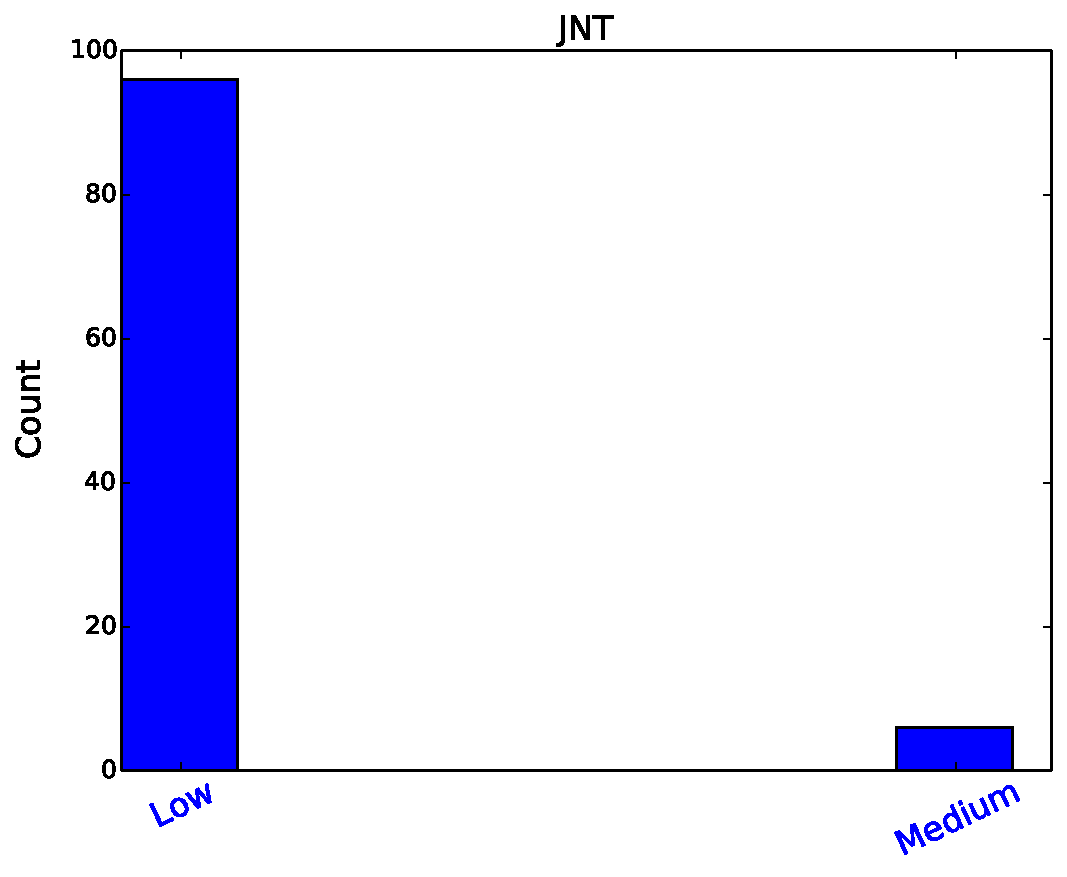
\includegraphics[width=0.29\textwidth]{../Code/ClassificationPlots/JNT_bar.pdf}\hfill
  
  }
        \qquad
\subfloat[][]{

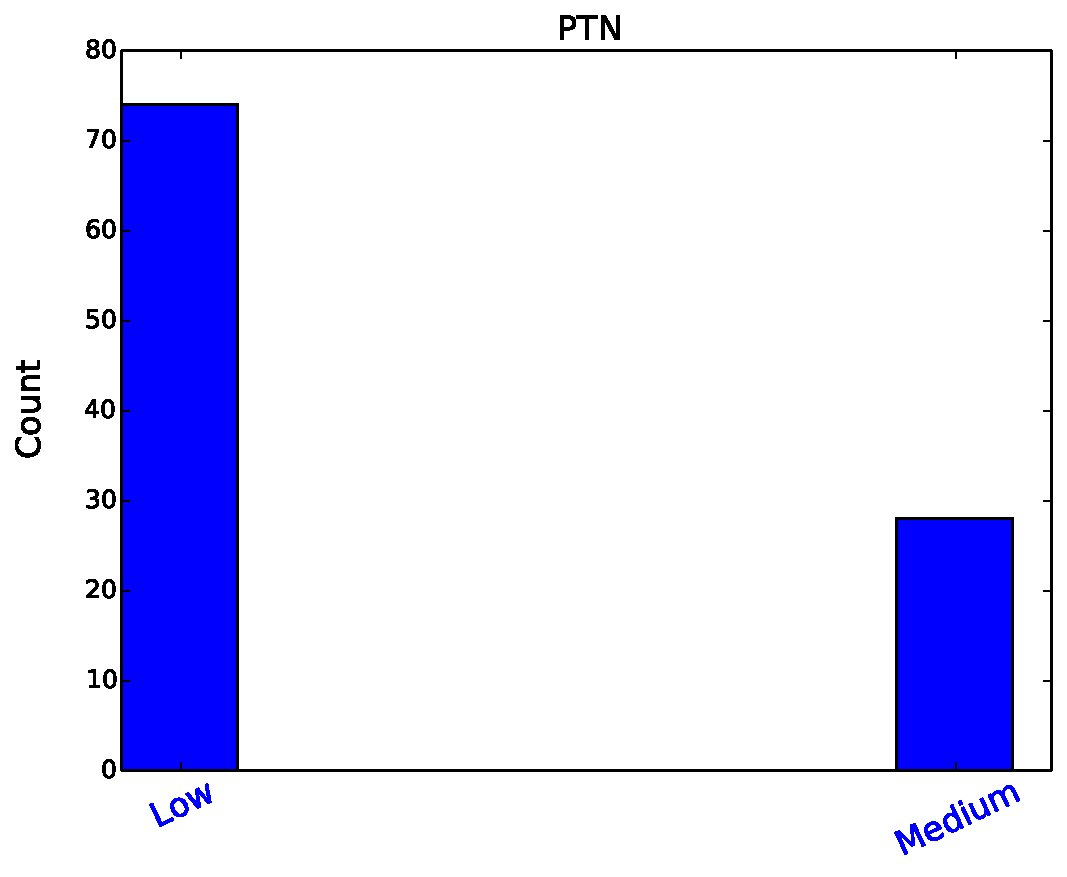
\includegraphics[width=0.29\textwidth]{../Code/ClassificationPlots/PTN_bar.pdf}\hfill
  
  }
          \qquad
\subfloat[][]{

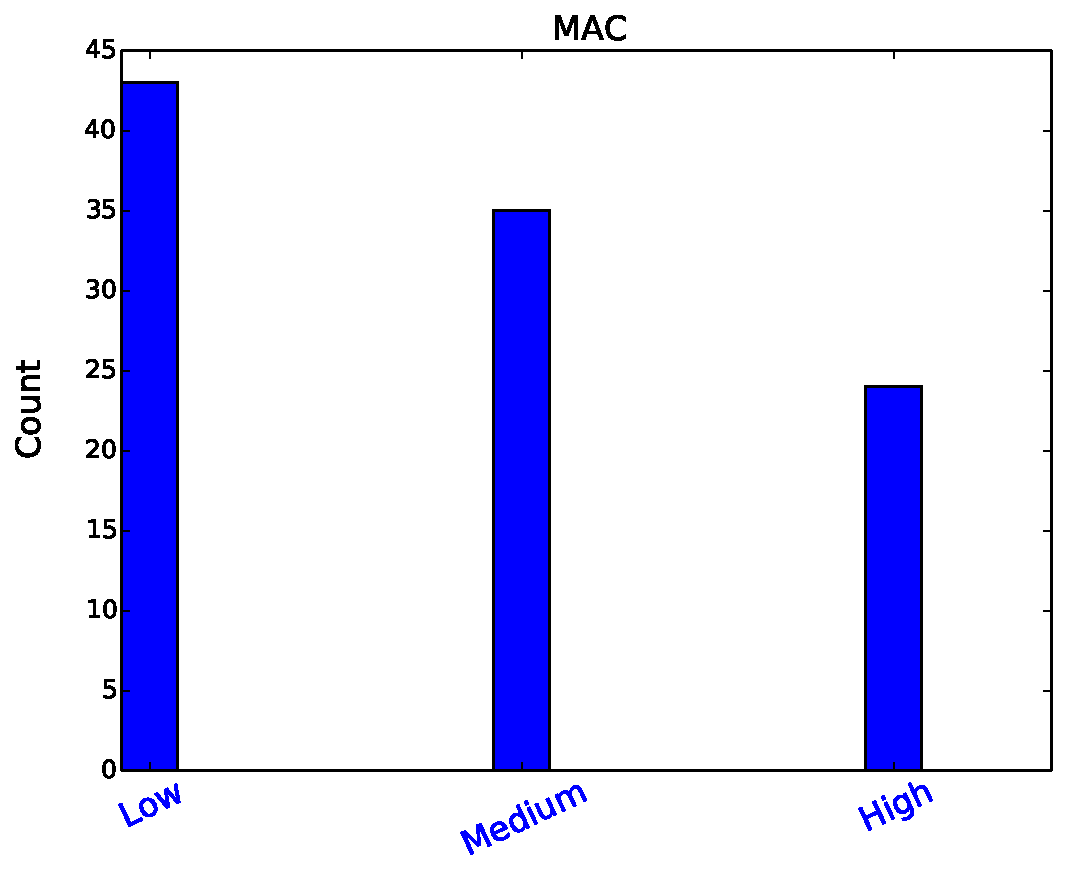
\includegraphics[width=0.29\textwidth]{../Code/ClassificationPlots/MAC_bar.pdf}\hfill
  
  }
\qquad
\subfloat[][]{

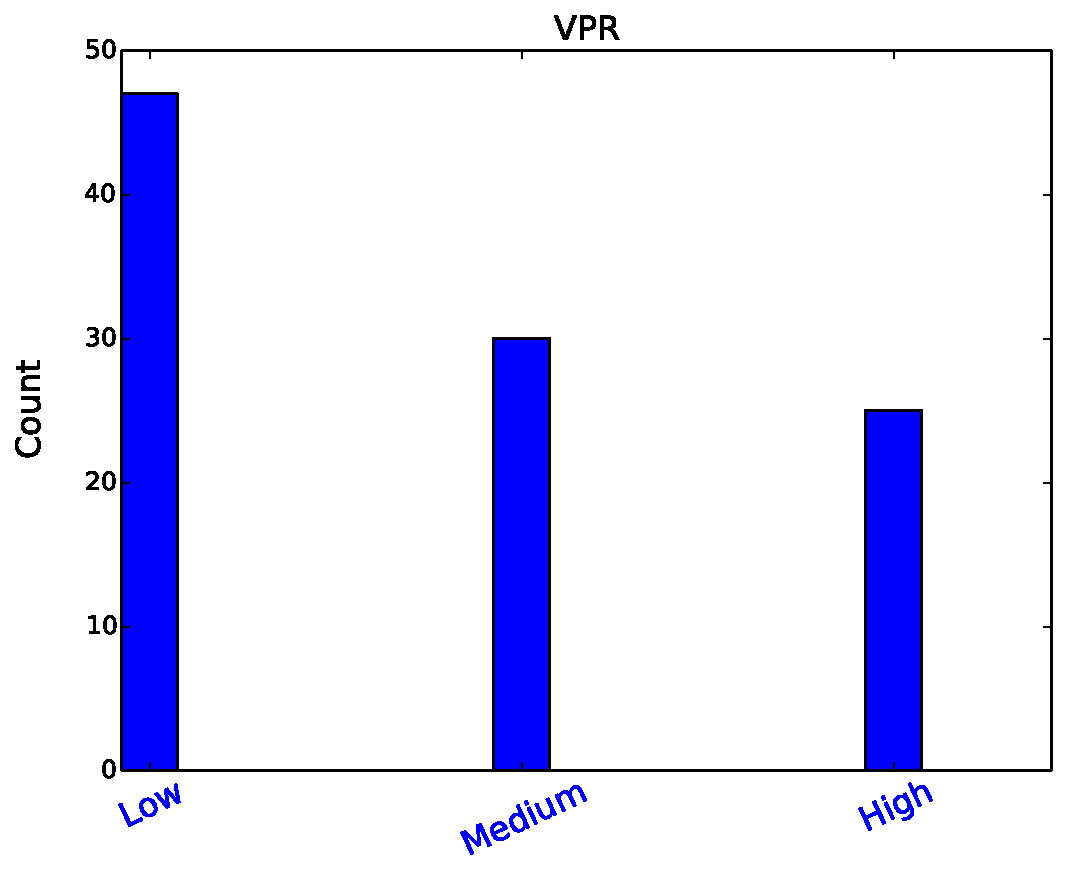
\includegraphics[width=0.29\textwidth]{../Code/ClassificationPlots/VPR_bar.pdf}\hfill

  
  }
  \qquad
\subfloat[][]{

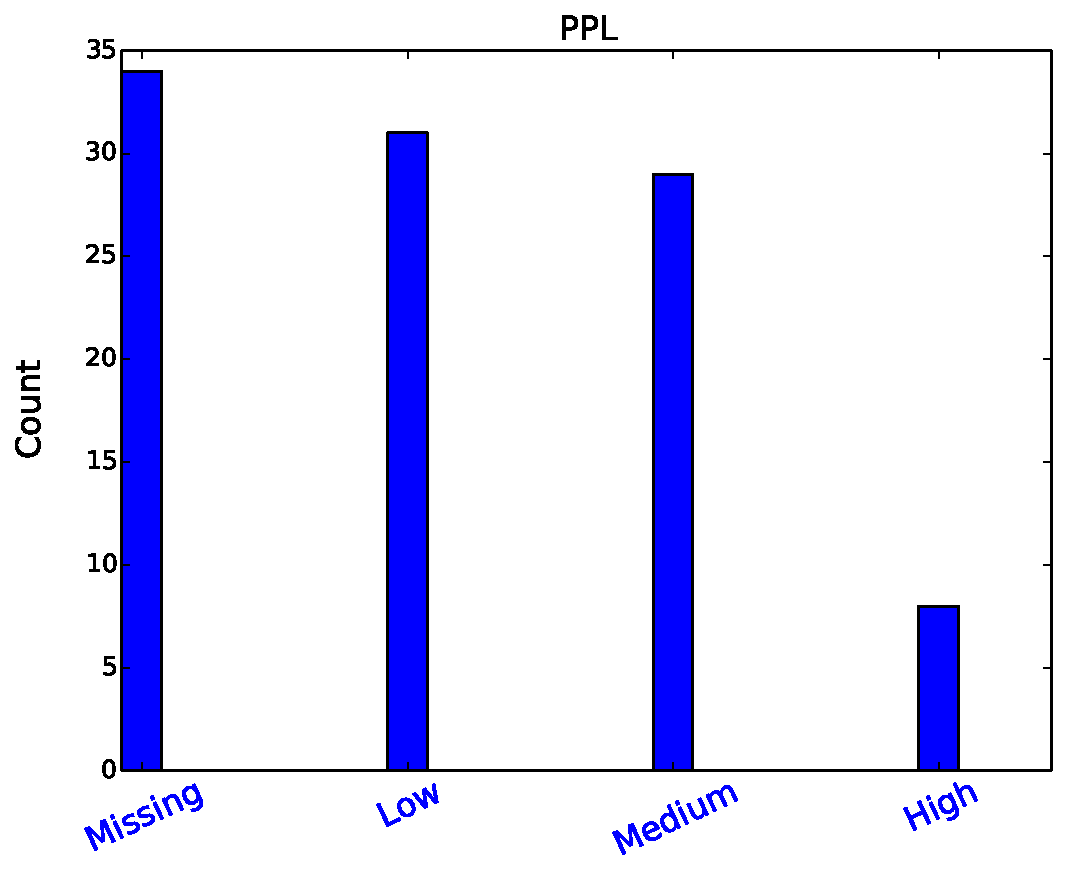
\includegraphics[width=0.29\textwidth]{../Code/ClassificationPlots/PPL_bar.pdf}\hfill

  
  }
\qquad
\subfloat[][]{

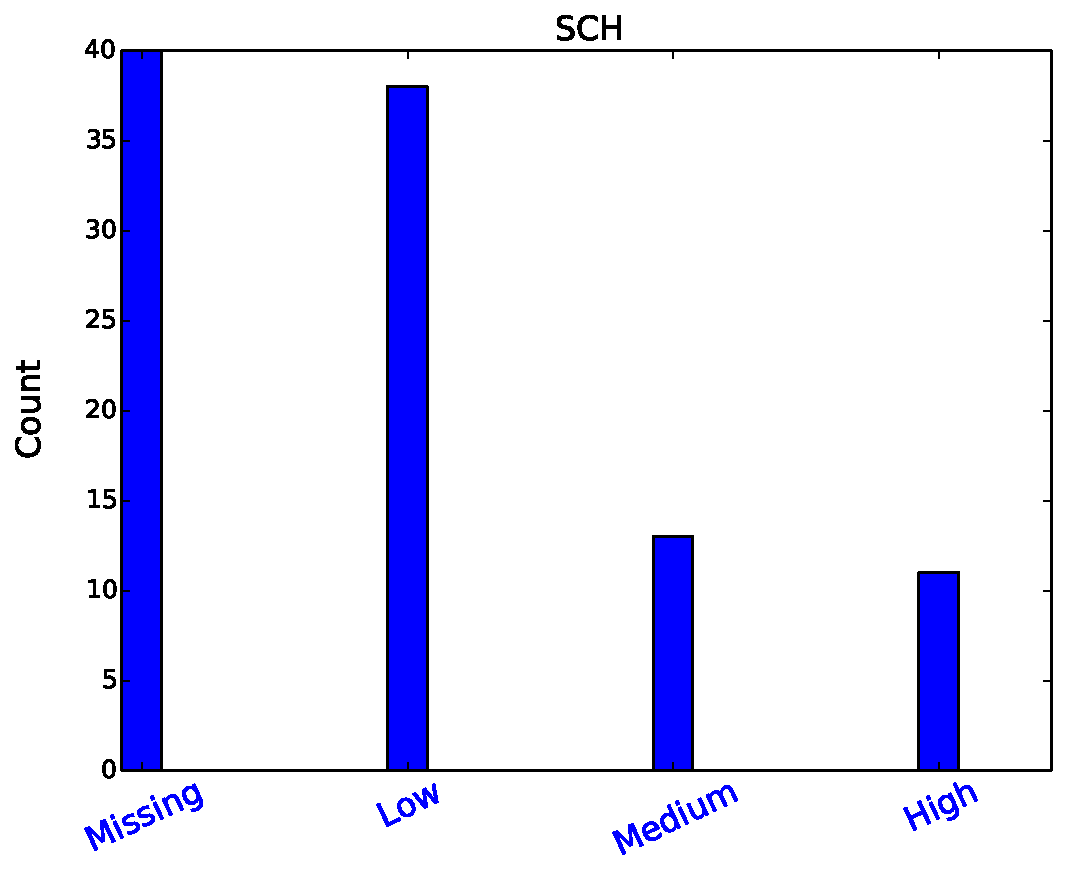
\includegraphics[width=0.29\textwidth]{../Code/ClassificationPlots/SCH_bar.pdf}\hfill

  
  }
  \qquad
\subfloat[][]{


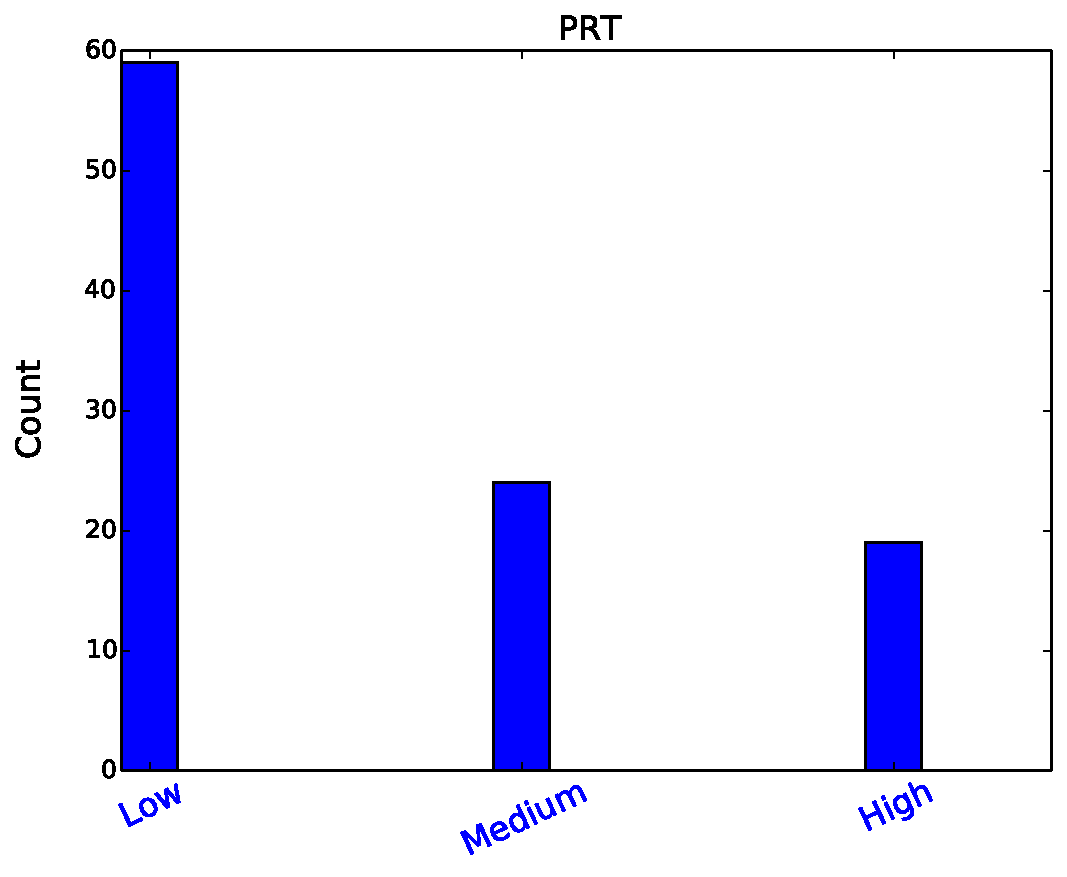
\includegraphics[width=0.29\textwidth]{../Code/ClassificationPlots/PRT_bar.pdf}\hfill

  
  }
  \qquad
\subfloat[][]{


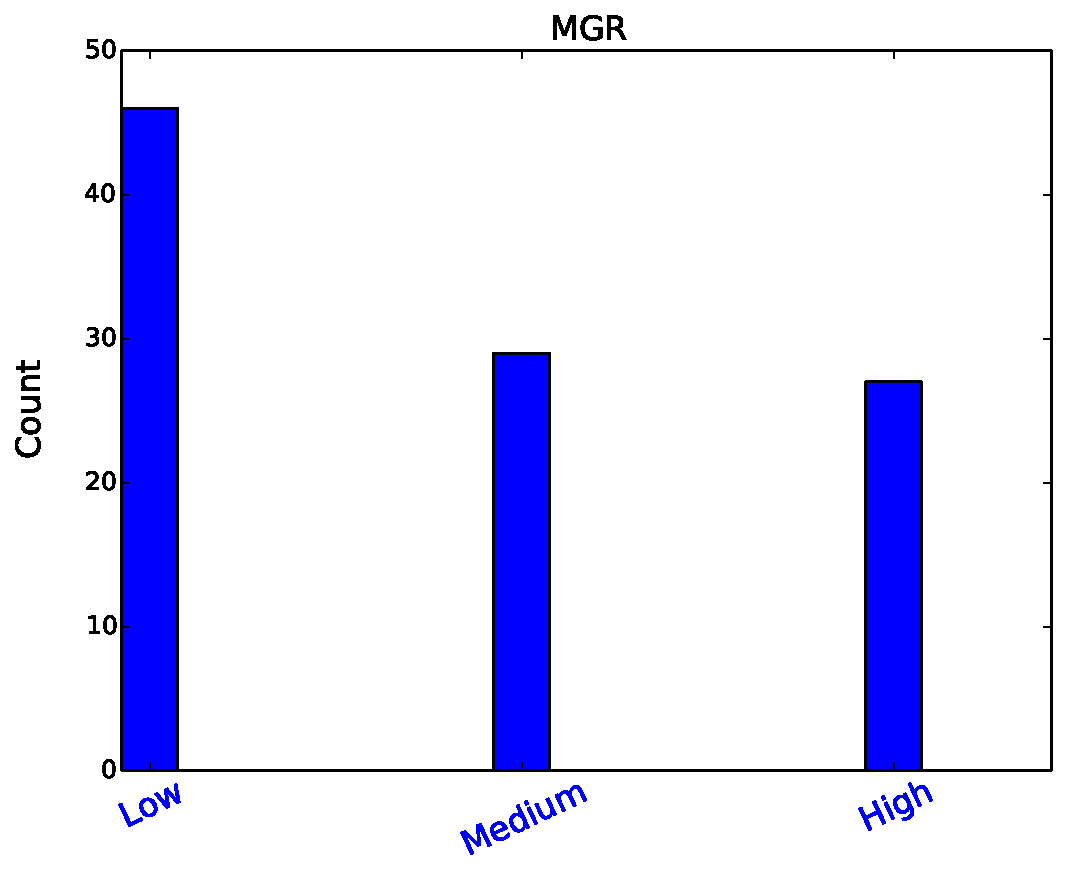
\includegraphics[width=0.29\textwidth]{../Code/ClassificationPlots/MGR_bar.pdf}\hfill

  
  }
  
  \end{figure}
  %TEMP END FOR PAGE SPLIT%
  \begin{figure}[H] \ContinuedFloat
  \centering
\subfloat[][]{
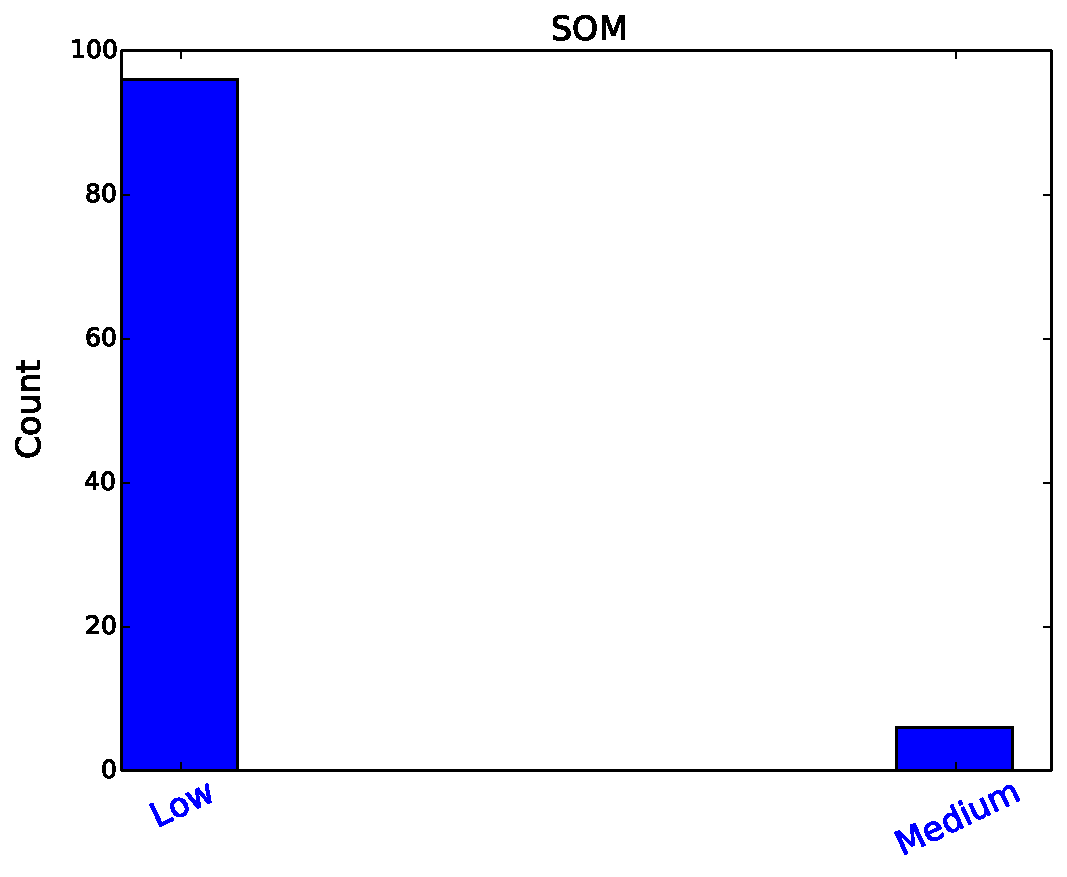
\includegraphics[width=0.29\textwidth]{../Code/ClassificationPlots/SOM_bar.pdf}\hfill

  
  }
 \qquad
\subfloat[][]{


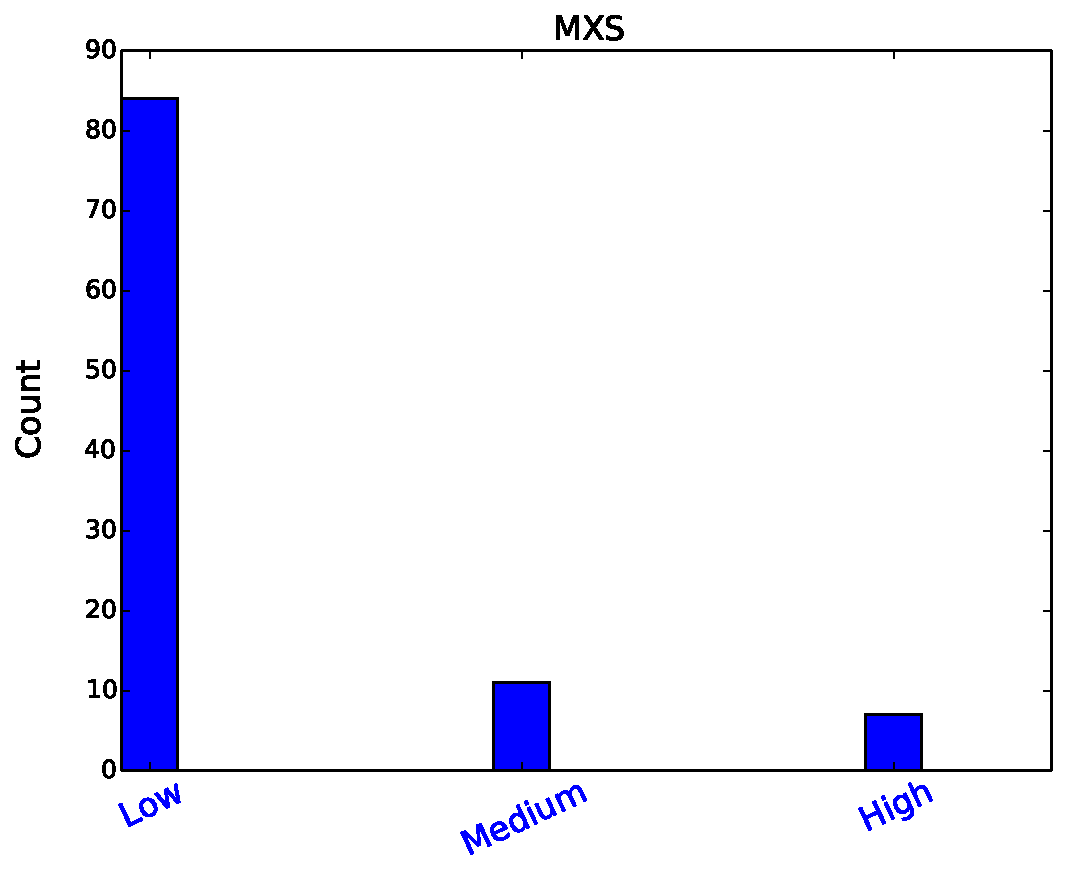
\includegraphics[width=0.29\textwidth]{../Code/ClassificationPlots/MXS_bar.pdf}\hfill
  
  }
   \qquad
\subfloat[][]{


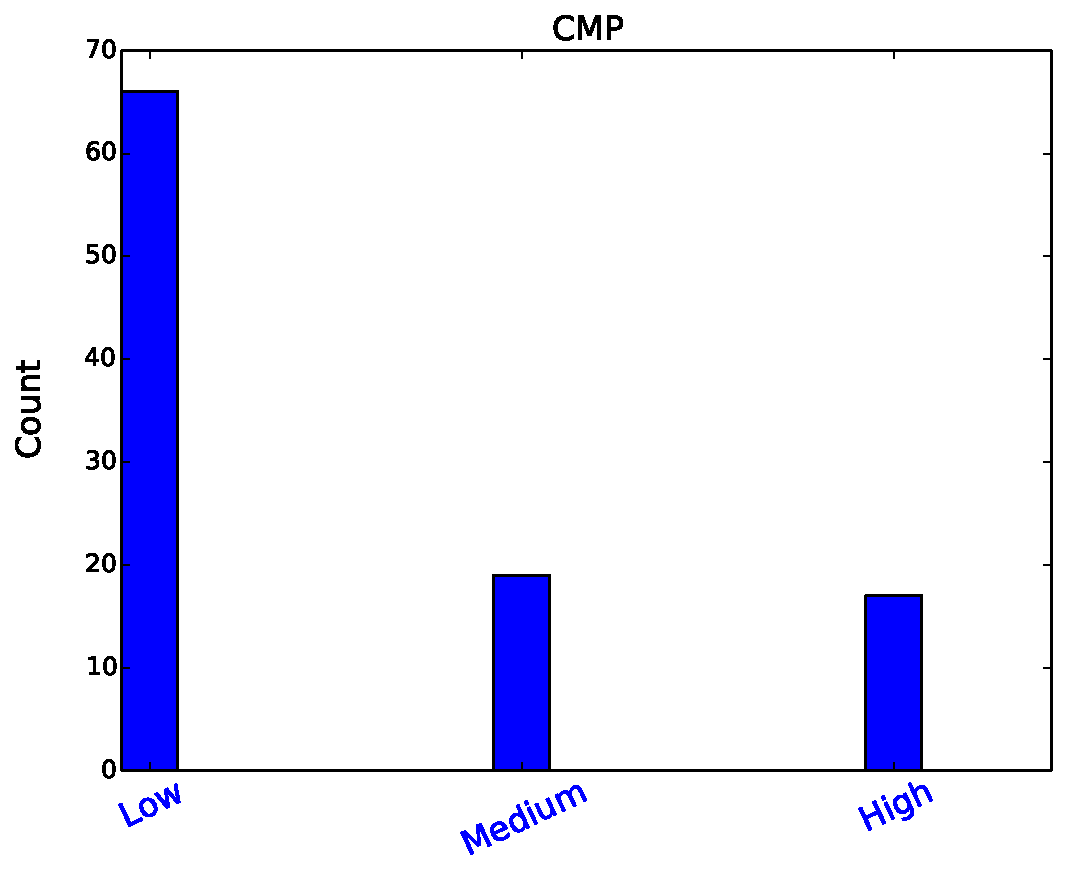
\includegraphics[width=0.29\textwidth]{../Code/ClassificationPlots/CMP_bar.pdf}\hfill
  
  }
   \qquad
\subfloat[][]{
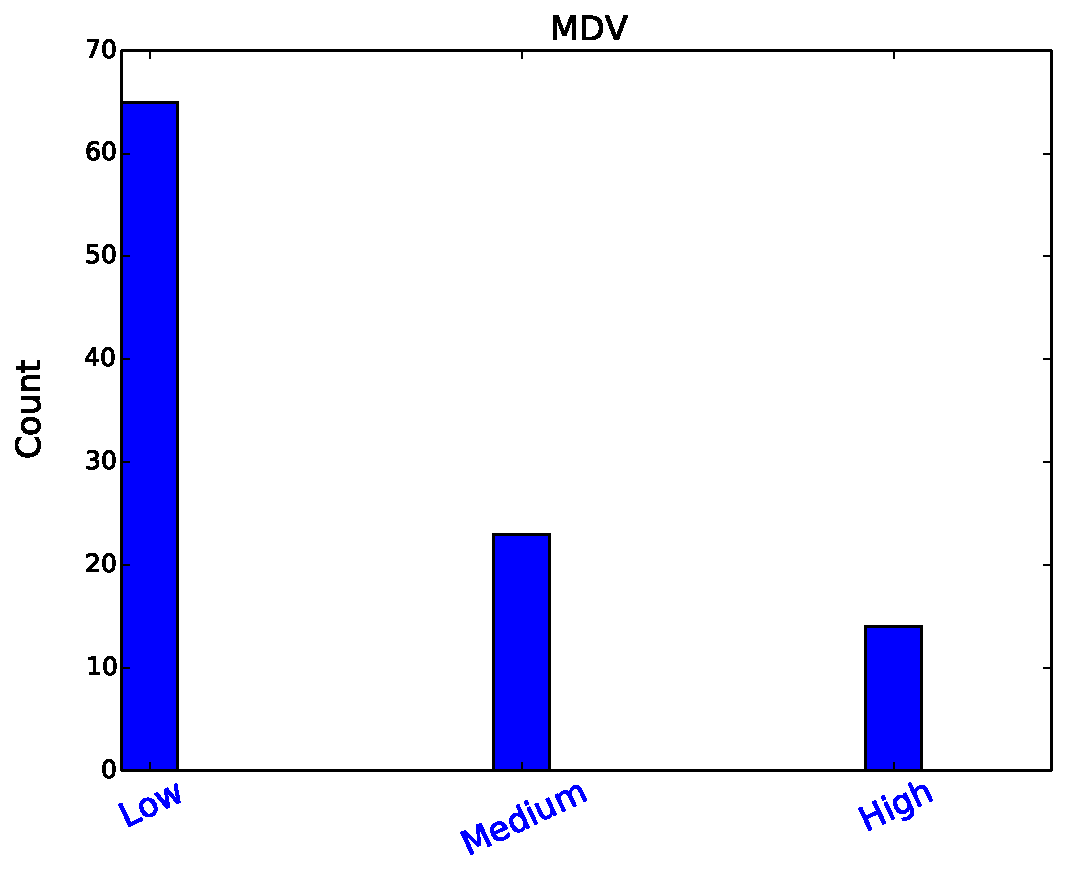
\includegraphics[width=0.29\textwidth]{../Code/ClassificationPlots/MDV_bar.pdf}\hfill
  
  }
     \qquad
\subfloat[][]{


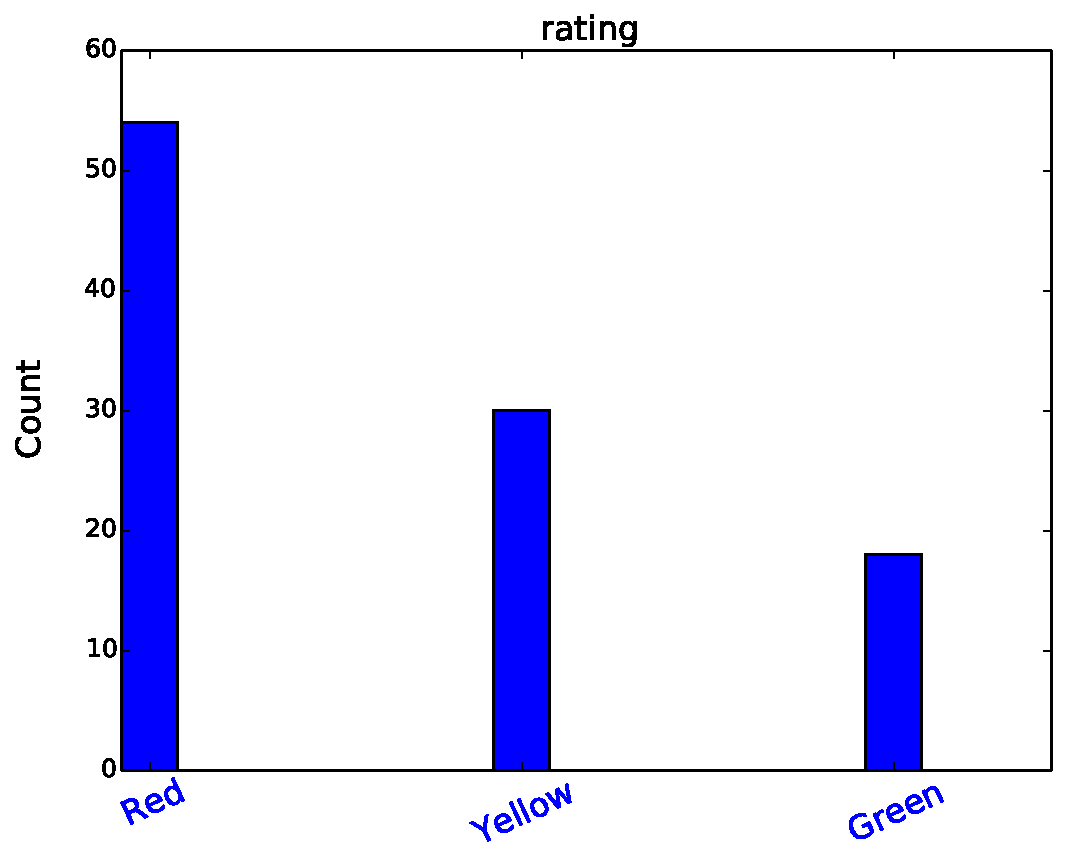
\includegraphics[width=0.29\textwidth]{../Code/ClassificationPlots/rating_bar.pdf}\hfill
}

  \caption{Frequency Tables for all attributes in the dataset.}%
  \label{fig:bars}%
\end{figure}




\end{homeworkProblem}

\clearpage
% To have just one problem per page, simply put a \clearpage after each problem
%----------------------------------------------------------------------------------------
%	PROBLEM 2
%----------------------------------------------------------------------------------------

\begin{homeworkProblem}[Problem \arabic{homeworkProblemCounter}: Association Analysis of Successful Companies (20 points) ]
Based on the results of the investment classifier, the firm would like to understand if there are any association rules for the attributes of a successful company. For example, are successful companies that have a good leadership team more likely to have better market positioning? These rules would allow them to better understand patterns across their investments and make recommendations for improvement.

To generate these rules, you have been asked to perform the following tasks:

\begin{enumerate}
\item	Create a subset of the original investment dataset that only contains the successful companies, i.e. green label.
\item	Explain the difference between support, confidence, and lift. How will changing the support and confidence change the discovered patterns?
\item Experiment with different values for support and confidence. What threshold do you recommend using for support and confidence?
\item	Identify 2-5 interesting rules generated using your selected support and confidence threshold. What is the interpretation of the rule? What is underlying rationale or reason for the rule, e.g. the diapers -> beer rule was because young fathers were sent to the store to buy diapers.
\item	What are some other potential applications of the generated rules? For example, would these rules be useful to the founder of a start-up company?
\end{enumerate}

\textbf{Extra Credit}:\\
 Repeat the rule generation process using only the unsuccessful companies, i.e. Red label. Compare and contrast the results to the association rules for the successful companies.

	
\noindent\rule{16cm}{0.9pt}
		
\large{\textbf{\underline{Answer:}}}
\begin{enumerate}

\item We can use Python and the \texttt{pandas} library in order to create a dataset that contains only the \emph{green} labeled companies. 

\item  Let $X,Y$ be two disjoint itemsets. Then we measure the strength of the association rule $X\rightarrow Y$, by using metrics such as \textbf{support, confidence} and \textbf{lift}. More precisely, the support is defined as: 
\[ s(X\rightarrow Y) = \frac{\sigma (X\cup Y)}{N} \]
,and measures the \textbf{fraction of transactions that contain both $X$ and $Y$} \\

We define the confidence of the rule to be: 
\[ c(X\rightarrow Y) = \frac{\sigma (X\cup Y)}{\sigma(X)} \]
,which measures \textbf{how frequently items included in $Y$ appear in rules that contain $X$.}

Finally, lift is defined as: 
\[ Lift= \frac{c(X\rightarrow Y)}{s(Y)} = 
\frac{N s(X\cup Y) / \sigma(X) }{s(Y)} =
\frac{ s(X\cup Y)  }{s(Y) \sigma(X) / N }=  
\frac{ s(X\cup Y)  }{s(Y) s(X) } \]
, which can be thought of as a ratio of  \textbf{``actual''$/$``expected''}, thus we would like to pick rules for which $Lift \gg 1$. Also, if $Lift=1 \implies s(X\cup Y) = s(Y) s(X)$ which implies statistical independence, therefore we would like to choose rules for which lift as large as possible.\\

Since we are using the \textbf{Apriori Algorithm} to find interesting association rules, setting the support to a small number (close to $0$) will result in a much larger set of candidate rules to be searched. Moreover, as we decrease the support, the produced rules will tend to be more infrequent, thus we could come across rules that \textbf{occurred by chance}. \\

As we decrease the confidence (values close to $0$), we will produce rules which are not very \textbf{reliable}. More precisely, the higher the confidence, the more likely it is for $Y$ to be present in transactions that contain $X$.

\item We find the best threshold for the support and confidence heuristically, therefore we need to experiment with many different values. Using \texttt{R} we produce Figure \ref{fig:rules} where we see that there exist no rules which have support less than $0.7$ and greater than $0.13$. Also, we observe that the highest lift value ($\approx 15$) is obtained for a small support and very large confidence. As a result, the threshold that we would recommend would be $s\approx 0.07$ and $c\approx 0.98$.


\begin{figure}[H]
	\begin{center}
		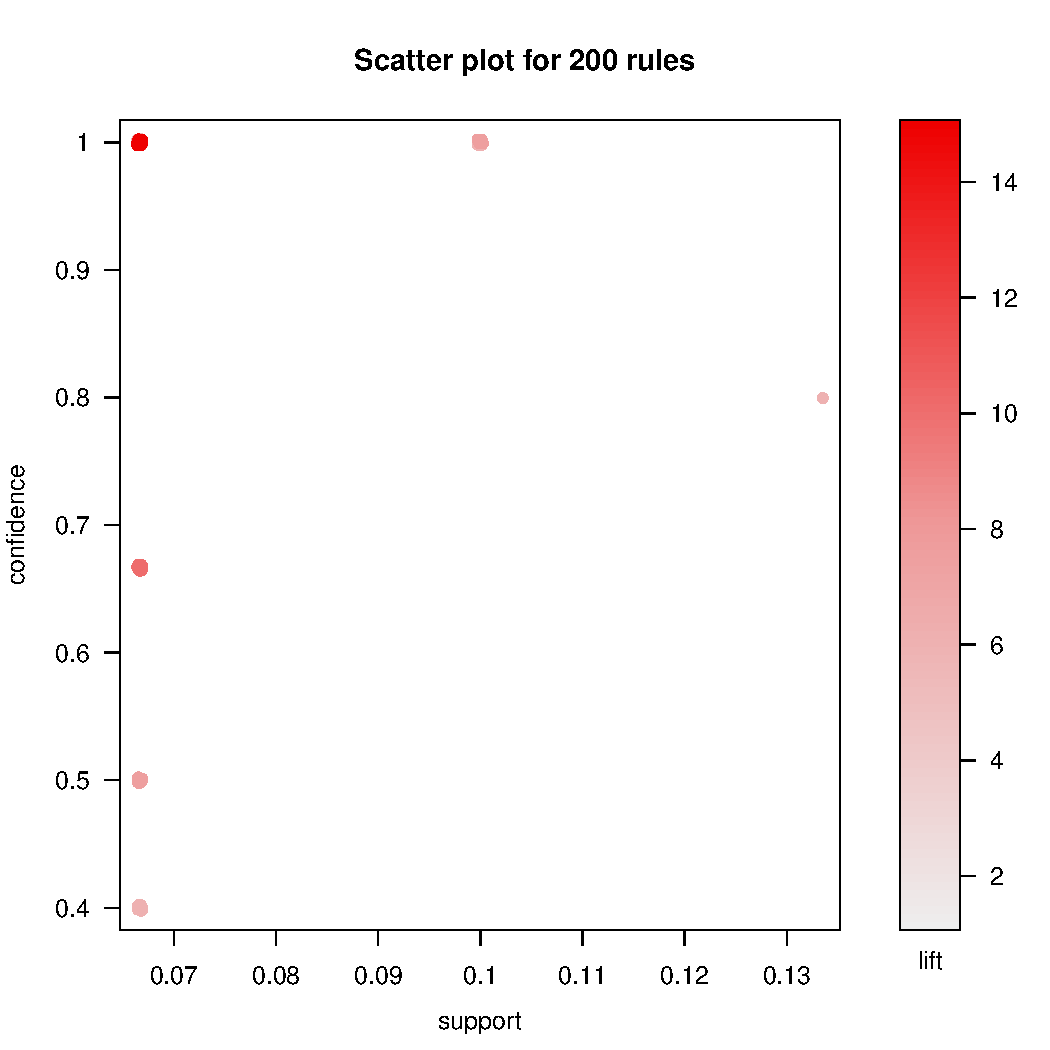
\includegraphics[width=0.6\textwidth]{../Code/ClassificationPlots/rules_green.pdf}\hfill
 	\end{center}
  	\caption{Scatter plot displaying the support, confidence and lift of $200$ rules for the \textbf{green} labeled companies.}
  	\label{fig:rules}
\end{figure}

\item We present three interesting rules along with their interpretation in the following list:

\begin{enumerate}
\item $\{CMP=low, GRO=medium, SCH=high\}  \Longrightarrow \{TCH=medium\}$ : \\

This rule achieves a support, confidence and lift equal to $s= 0.067, c= 1, lift= 15$. It implies that within the successful startup companies, it is observed that in a non competitive landscape (\emph{low}), with  \emph{medium} ability to react to risk and a \emph{high} quality of supply chain integration, a company often possesses of \emph{medium} quality of technical team. \\

\item $\{SCH=low, CMP=medium\}  \Longrightarrow \{VPR=high\}$ : \\

This rule achieves a support, confidence and lift equal to $s= 0.067, c= 1, lift= 7.5$. It implies that with a \emph{low} quality of supply chain integration and \emph{medium} level of competitive landscape, a successful company can obtain a \emph{high} value position. \\

\item $\{EXP=low, JNT=low, CPL=medium, MAC=high, SCH= high\}  \Longrightarrow \{INO=medium\}$:  \\	

This is the lengthiest rule and it achieves a support, confidence and lift equal to $s= 0.1, c= 1, lift= 7.5$. It implies that with \emph{low} leadership and joint team experience, \emph{medium} levels of team completeness and \emph{high} levels of market acceptance and supply chain integration, a succesful company often manages to have a \emph{medium} ability to innovate.

\end{enumerate}


\item These rules could have many different applications. First, the founder of a startup company would know the ``recipe'' for a successful company. For instance, by observing the aforementioned rules, a company would know that in order to obtain a high value position, it would need to first have  a medium level of competitive landscape. Moreover, these results could also be of great value for \textit{Redwood Capital},  since it can more easily identify successful companies by examining if they satisfy common rules that other successful companies satisfy.

\end{enumerate}

\textbf{Extra Credit}: \\

In order to repeat the same procedure for the unsuccessful companies we first need to find the appropriate threshold values for the support and confidence. Using Figure \ref{fig:rules_red} we see that the distribution of rules with large lift values is different from before. We get many rules with high lift values as we vary the support between $0.03 \leq s \leq 0.04$ and we keep the confidence fixed to approximately $1$.  As a result, we focus on rules that have $s\approx 0.035$ and $c\approx 1$.

\begin{figure}[H]
	\begin{center}
		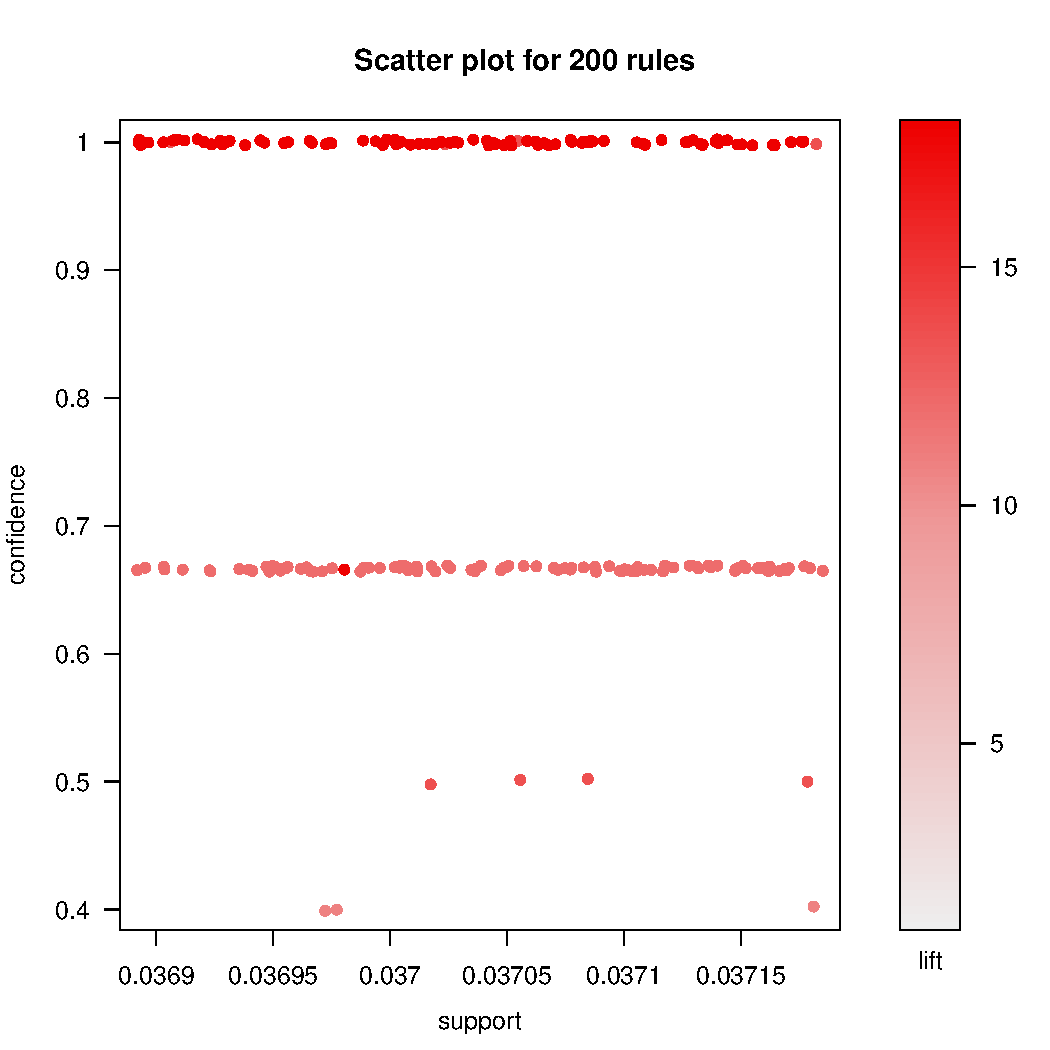
\includegraphics[width=0.6\textwidth]{../Code/ClassificationPlots/rules_red.pdf}\hfill
 	\end{center}
  	\caption{Scatter plot displaying the support, confidence and lift of $200$ rules for the \textbf{red} labeled companies.}
  	\label{fig:rules_red}
\end{figure}

Some interesting rules that we see are the following:
\begin{enumerate}
\item $\{MDV=low, MKT=low, MAC=low\}  \Longrightarrow \{CMP=high\}$:  \\

This rule achieves a lift score of $18$ and demonstrates an common reason why many startup companies fail.  If a company has minimal market experience, market acceptance as well as market diversity and functions in a very competitive landscape, it is also very likely to go bankrupt. 

\item $\{MDV=low, MKT=low, GRO=medium\}  \Longrightarrow \{EXP=medium\}$:  \\

This rule also achieves a lift score of $18$. It shows that in unsuccessful companies, very often, low market experience in combination with low market diversity and inability to evaluate risk well, occur together with poor leadership experience. Without leadership and correct decision making, a company is very likely to go bankrupt, therefore it is labeled as ``red''. 

\item $\{PTN=low, GRO=medium\}  \Longrightarrow \{CMP=high\}$:  \\

This rule also achieves a lift score of $13$ and is similar to the first rule. It describes that without intellectual product rights and a medium ability to evaluate risks in a competitive landscape, a start up company can often fail.   
\end{enumerate}

\textbf{In general}, comparing the rules generated for both datasets, we see \textbf{patterns} that successful (green) and unsuccessful (red) startup companies follow. We see that the ability to \textbf{innovate} and have a good \textbf{technical team} can often lead companies to success. Nevertheless, we observe that a \textbf{competitive landscape environment} can lead to failure for a newly formed company. 

 \end{homeworkProblem}
\clearpage

%----------------------------------------------------------------------------------------
%	PROBLEM 3
%----------------------------------------------------------------------------------------
\begin{homeworkProblem}[Problem \arabic{homeworkProblemCounter}: Clustering Crowdfunded Projects on Kickstarter (40 Points) ]

Crowdfunding is an alternative source of funding for start-up companies where small investments, e.g. $100\$ $, are made by thousands of independent investors. These investments are typically managed through a crowdfunding portal, such as Kickstarter and Indie-Go-Go, where companies, or individuals, can post projects that they would like people to fund. \\

The crowdfunding market is potentially a new emerging investment opportunity for Redwood Capital. In addition to making several multi-million dollar investments every year, they could make small investments in hundreds of companies to diversify their portfolio and reduce risk. However, not all of the projects on crowdfunding sites are good candidates for commercialization. For example, projects often include humanitarian projects and art projects which would not be suitable for profit motivated investment firm like Redwood Capital. \\

The firm would like to further investigate these crowd-funding sites to see what kinds of projects are being funded and if they are a viable investment opportunity. To this end, they have collected a dataset of 4,000 projects from the popular crowd-funding site Kickstarter. 

The dataset contains the following attributes:
\begin{itemize}
\item	Project Title
\item 	Description
\item	Amount Funded
\item	Project Goal
\item	Project Category
\item	Type of Currency
\item	Location
\item	Number of Backers
\end{itemize}

You have been asked to perform the following tasks related to understanding the different groups of projects that are being funded on Kickstarter:
\begin{enumerate}
\item	First, remove the Project Title and Description fields from the dataset. Perform your EDA process on the remaining attributes and format the results into a well-structured report. Perform any data pre-processing steps (cleaning, transformation, etc.) necessary for addressing data quality issues that were discovered during the EDA process.
\item	The firm has asked you to explain the differences between the following popular clustering algorithms: K-Means, DB-Scan, Hierarchical Clustering, and Mixture Models (EM). In particular, how do these algorithms with respect to computational complexity, types of clusters that they can find, and interpretability?
\item	Before you start, the firm would like a written statement of your process for cluster analysis. (Hint: The process might include the steps such as visualizing the data or reviewing clusters with domain experts)
\item	Then, they would like you to apply your cluster analysis process to the collected data-set and format the results into a well-structured report.
\item	Identify 1-2 clusters of projects that would be good candidates for the firm to investigate further. Provide a brief summary description for each candidate cluster, e.g. video game projects developed in San Jose.
\end{enumerate}

\textbf{Extra Credit}:\\
 Create an additional set of attributes based on the project description and repeat your process for cluster analysis.

\noindent\rule{16cm}{0.9pt}
		
\large{\textbf{\underline{Answer:}}}
 \begin{enumerate}
 \item We follow a similar approach to Problem 1 in order to analyze the categorical variables \texttt{location}, \texttt{category} and \texttt{currency} . As far as the numerical variables are concerned, our Exploratory Data Analysis will consist of a combination of \textbf{visual} and \textbf{quantitative} tools to answer important questions for each selected attribute in our dataset. More precisely, for each attribute we will look into descriptive statistics such as the \textbf{typical value}, the \textbf{spread} for a typical value and whether it affects other attributes (\textbf{correlation}). Moreover, we will employ visual tools in order to estimate a good distributional fit for the data but also determine the existence of outliers (\textbf{histogram, box plots}). Also, we will use a combination of visual tools and descriptive statistics (\textbf{scatter plot, correlation}) to determine the co-linearity of attributes.

 
 \begin{figure}[H]
 \centering
 \caption{Pearson Correlation Matrix for all numeric attributes}
 \begin{tabular}{lrrr}
\toprule
{} &  amount\_funded &  project\_goal &  number\_backers \\
\midrule
amount\_funded  &       1.000000 &      0.436182 &        0.717896 \\
project\_goal   &       0.436182 &      1.000000 &        0.444587 \\
number\_backers &       0.717896 &      0.444587 &        1.000000 \\
\bottomrule
\end{tabular}
\label{table:corr_martrix}
\end{figure}

We first analyze the \textbf{numeric attributes} and for each attribute we discover the following information:\\
\texttt{amount\_funded}:
\begin{enumerate}
\item \textsc{Typical Value}: Calculating the mean for this attribute we get that the average score is approximately $289,992$
\item \textsc{Spread}: Approximately, the standard deviation (sample) for this data is $711,936$. Since significant outliers exist in this attribute a better measure of dispersion is $mad=67,354$
\item \textsc{Distributional fit}: Drawing a histogram of the data we see that the distribution looks very skewed to the right (i.e. few data points have extremely large values, see Fig. \ref{fig:hists})
\item  \textsc{Correlation}: Referring to Table \ref{table:corr_martrix} and Figure \ref{fig:hists},  we see that \texttt{amount\_funded} is most strongly positively correlated with  \texttt{number\_backers}. This is logical since we would expect that increasing the number of backers would also increase the total amount funded.
\item 	\textsc{Outliers}: There exist some outliers which is evident from the magnitude of the measures of dispersion. Also outliers become apparent by looking at the histogram in Figure \ref{fig:hists}.
\end{enumerate}

\texttt{project\_goal}:
\begin{enumerate}
\item \textsc{Typical Value}: Calculating the mean for this attribute we get that the average score is approximately $61,752$
\item \textsc{Spread}: Approximately, the standard deviation (sample) for this data is $126,671$. Similarly to before, since outliers exist in this attribute a better measure of dispersion is $mad=20,000$
\item \textsc{Distributional fit}: Drawing a histogram of the data we see that the distribution looks very skewed to the right (i.e. few data points have extremely large values, see Fig. \ref{fig:hists})
\item  \textsc{Correlation}: Referring to Table \ref{table:corr_martrix} and Figure \ref{fig:hists},  we see that \texttt{project\_goal} is not significantly correlated with any of the other variables.
\item 	\textsc{Outliers}: There exist some outliers which is evident from the magnitude of the measures of dispersion. Also outliers become apparent by looking at the histogram in Figure \ref{fig:hists}.
\end{enumerate}

\texttt{number\_backers}:
\begin{enumerate}
\item \textsc{Typical Value}: Calculating the mean for this attribute we get that the average score is approximately $3,582$
\item \textsc{Spread}: Approximately, the standard deviation (sample) for this data is $7,316$. Similarly to before, since outliers exist in this attribute a better measure of dispersion is $mad=671$
\item \textsc{Distributional fit}: Drawing a histogram of the data we see that the distribution looks very skewed to the right (i.e. few data points have extremely large values, see Fig. \ref{fig:hists})
\item  \textsc{Correlation}: As explained, this variable is most strongly correlated with \texttt{amount\_funded}.
\item 	\textsc{Outliers}: There exist some outliers which is evident from the magnitude of the measures of dispersion. Also outliers become apparent by looking at the histogram in Figure \ref{fig:hists}.
\end{enumerate}

Now we proceed to \textbf{clean} our dataset. First we need to explore whether our attributes contain \textbf{duplicates}. After querying the dataset, we find $7$ duplicate instances, whose names are summarized in Table \ref{table:dups}. We \textbf{remove the duplicates} from the dataset in order to perform clustering analysis.

 \begin{table}[H]
 \centering
 \caption{Titles of duplicate instances.}
 \begin{tabular}{c}
\toprule
{Title} \\
\midrule
Doug TenNapel Sketch Book Vol 2  \\
 Frame by Frame   \\
The Infinite Loop Tablet and Smartphone Stand \\
  Simple Bracket \\
                  THE BEST OF WDW - Volume 1 \\
 Aer Fit Pack: The Gym/Work Bag Designed for the City \\
     XRAY.FM - The little station with big ideas. \\
\bottomrule
\end{tabular}
\label{table:dups}
\end{table}

Based on our analysis, we know that there exist \textbf{outliers} in our numerical attributes. Therefore for all of our attributes we define $Q_{0}=10\%$ quantile and $Q_{1}=80\%$ quantile and then take the attributes which fall inside these quantiles. Following this process, we only keep the following values:

 \[  81,136 \leq \texttt{amount\_funded} \leq 20,3491 \]
  \[  18,000 \leq \texttt{project\_goal} \leq 50,000 \]
    \[  1,537 \leq \texttt{number\_backers}: \leq 2,752 \]


 After discarding outliers we still have not merged the attributes together in order to create a single dataframe. We notice, that since we have deleted many values, ``merging'' the columns back together would result in having many \textbf{empty} cells. Therefore, we decide to delete all datapoints that contain at least $1$ empty cell. That reduces significantly our datasets's size from $4,000$ instances to $1,013$. \\

The \textbf{reason behind} deleting all instances with at least one empty cell, is that we do not want any outliers in our dataset. More precisely, if an empty cell exists, then it means that its original value had been filtered out by the procedure we followed in the previous step (step $1$), and hence, it was an outlier. An \textbf{alternative} approach would be to replace every missing value with the mean of that attribute, but that would inevitably distort the data and introduce some bias. This is not necessary here, since the resulting dataset size is adequate to allow our model to discover meaningful clusters.\\


We now analyze the \textbf{categorical} variables of our dataset. By looking at Table \ref{table:items} we see that there is a large variety of combinations of values that the attributes take. More precisely, we observe all the attributes are multimodal, since there does not exist a value that occurs much more frequently than others. Moreover, by looking at Table \ref{table:items} we see that the most frequent location (\textbf{mode}), category and currency are \textbf{San Francisco, Product Design} and \textbf{usd}, respectively. \\

 In order to use the categorical information in our clustering models we need to add new binary attributes to the dataset, but we first use \texttt{OpenRefine} to ensure that there are no \textbf{spelling inconsistencies}. The number of discrete values that  \texttt{location}, \texttt{category} and \texttt{currency} take are $806, 115, 9$, respectively. Evidently, if we encode all these variables as numerical the dimensionality of the problem would explode, leading to very sparse data (\emph{curse of dimensionality}). Heuristically, we choose the top $30$ most frequent items from the  \texttt{location} and \texttt{category} attributes, and we name the rest of the items of each attribute as \texttt{other\_location}, \texttt{other\_category}, respectively. As a result, we create $73$ new binary variables, out of which, $31$ correspond to location, $31$ correspond to category and $9$ correspond to currency. 


\vspace{1cm}

\begin{center}
\textsc{ \textbf{Appendix for Problem 3 Question 1} }
\end{center}

%%% TABLES %%%%
\begin{table}[H]%
  \centering
  \subfloat[][]{
  
\begin{tabular}{lr}
\toprule
 location &  count \\
\midrule
San Francisco, CA  &  280 \\
Los Angeles, CA    &  271\\
New York, NY     &      212\\
Seattle, WA          &  147\\
London, UK           &  132\\
Chicago, IL    &        121\\
Brooklyn, NY      &     103\\
Portland, OR           & 84\\
San Diego, CA   &        62\\
Toronto, Canada    &     60\\

\bottomrule
\end{tabular}

  }%
  \qquad
  \subfloat[][]{
\begin{tabular}{lr}
\toprule
category&  count \\
\midrule
Product Design&    773\\
Tabletop Games&    742\\
Video Games       &524\\
Hardware&          182\\
Technology&        152\\
Documentary&       124\\
Gadgets&           121\\
Design     &        99\\
Comics       &      79\\
Wearables    &      64\\
\bottomrule
\end{tabular}
  
  }
 \qquad
\subfloat[][]{


\begin{tabular}{lr}
\toprule
{currency} &  count \\
\midrule
usd&    3438 \\
gbp&     252\\
cad   &  128\\
eur      &96\\
aud&      52\\
sek   &   14\\
nzd     & 10\\
dkk       &7\\
chf       &3\\
\bottomrule
\end{tabular}
  }
\caption{Top 10 most frequent items for the \textbf{categorical} attributes.}
\label{table:items}
\end{table}

\vspace{2cm}

\begin{figure}[H]
\centering
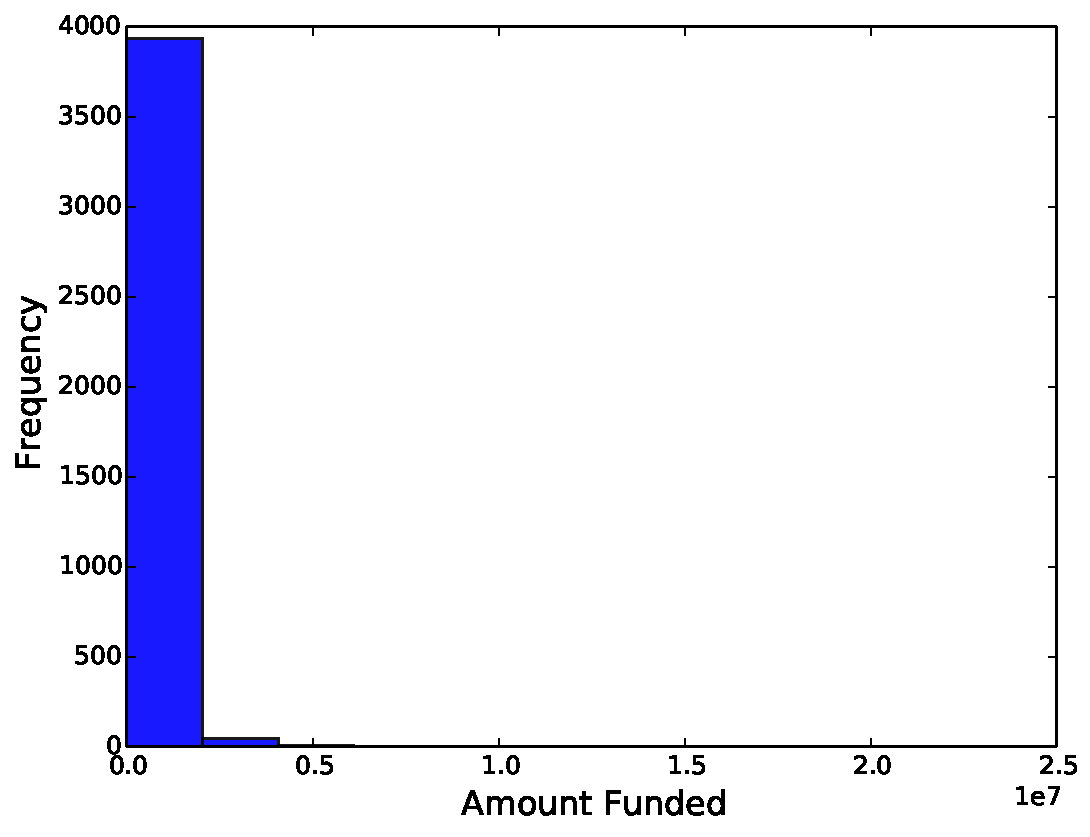
\includegraphics[width=.45\textwidth]{../Code/ClusteringPlots/amt_hist.pdf}\hfill
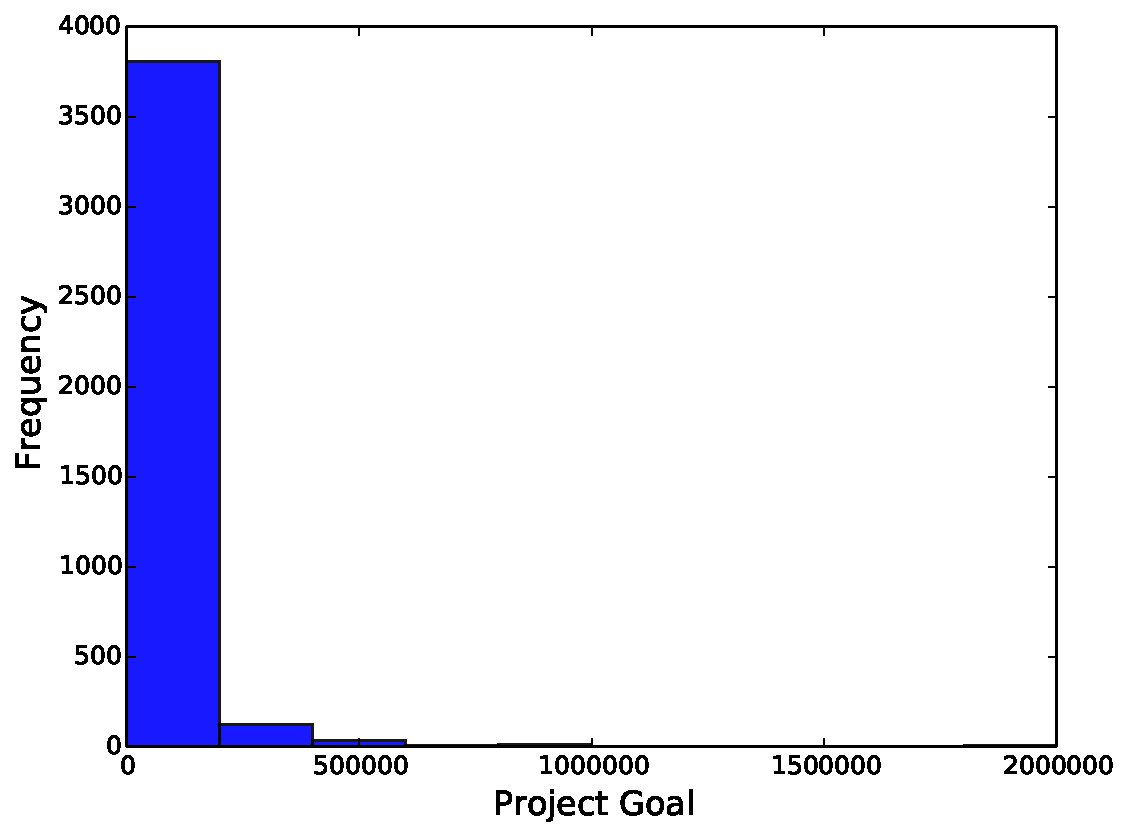
\includegraphics[width=.45\textwidth]{../Code/ClusteringPlots/prj_hist.pdf}\hfill
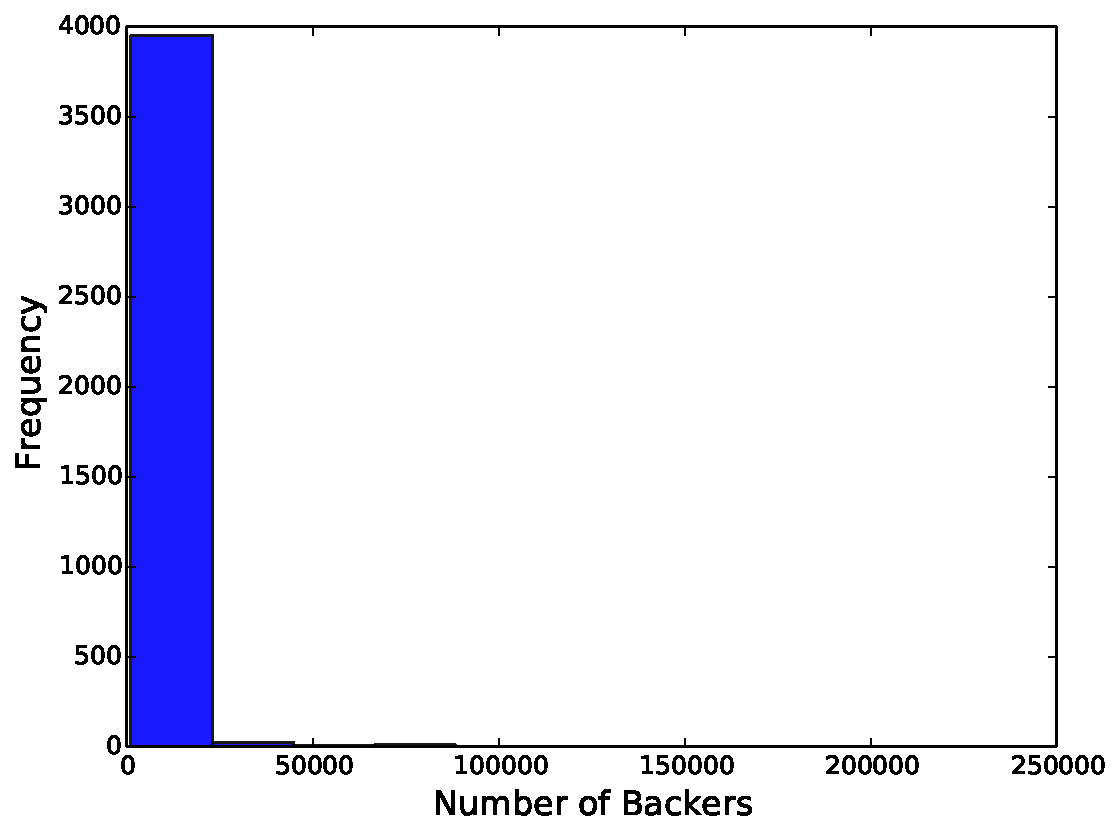
\includegraphics[width=.45\textwidth]{../Code/ClusteringPlots/backers_hist.pdf}\hfill
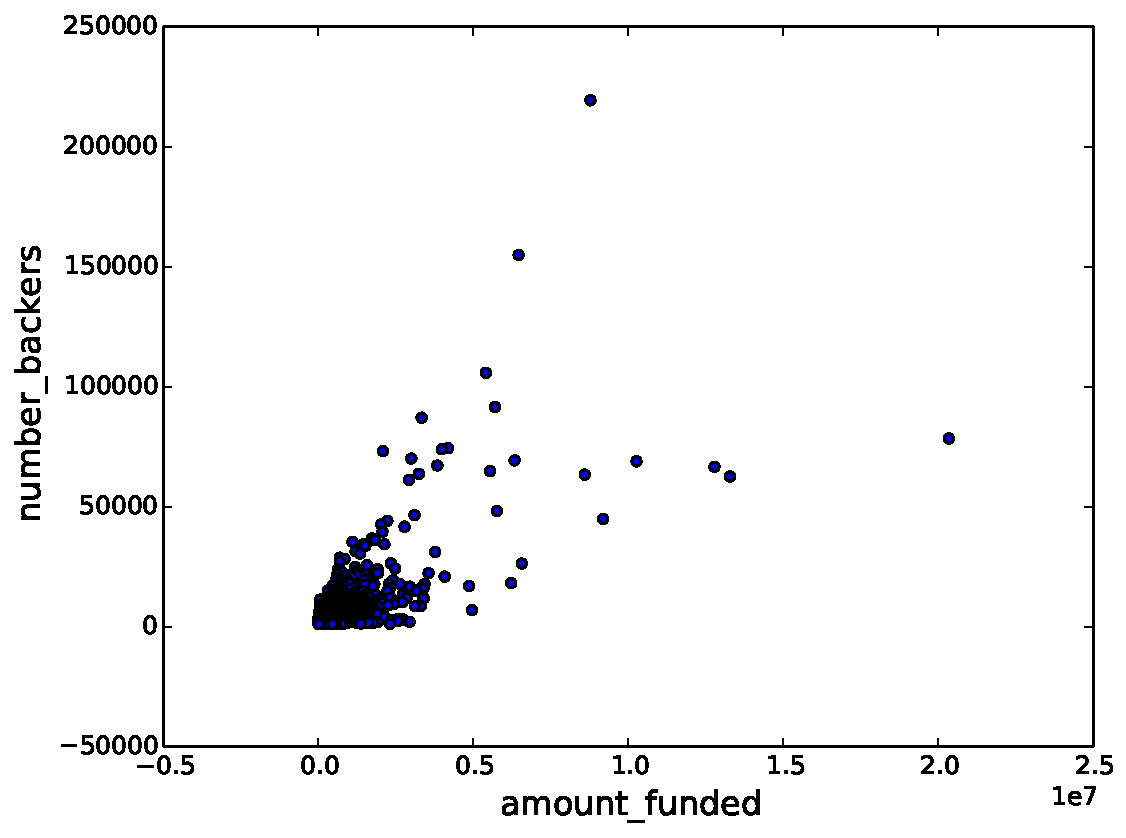
\includegraphics[width=.5\textwidth]{../Code/ClusteringPlots/amount_fundednumber_backers_scatter.pdf}\hfill
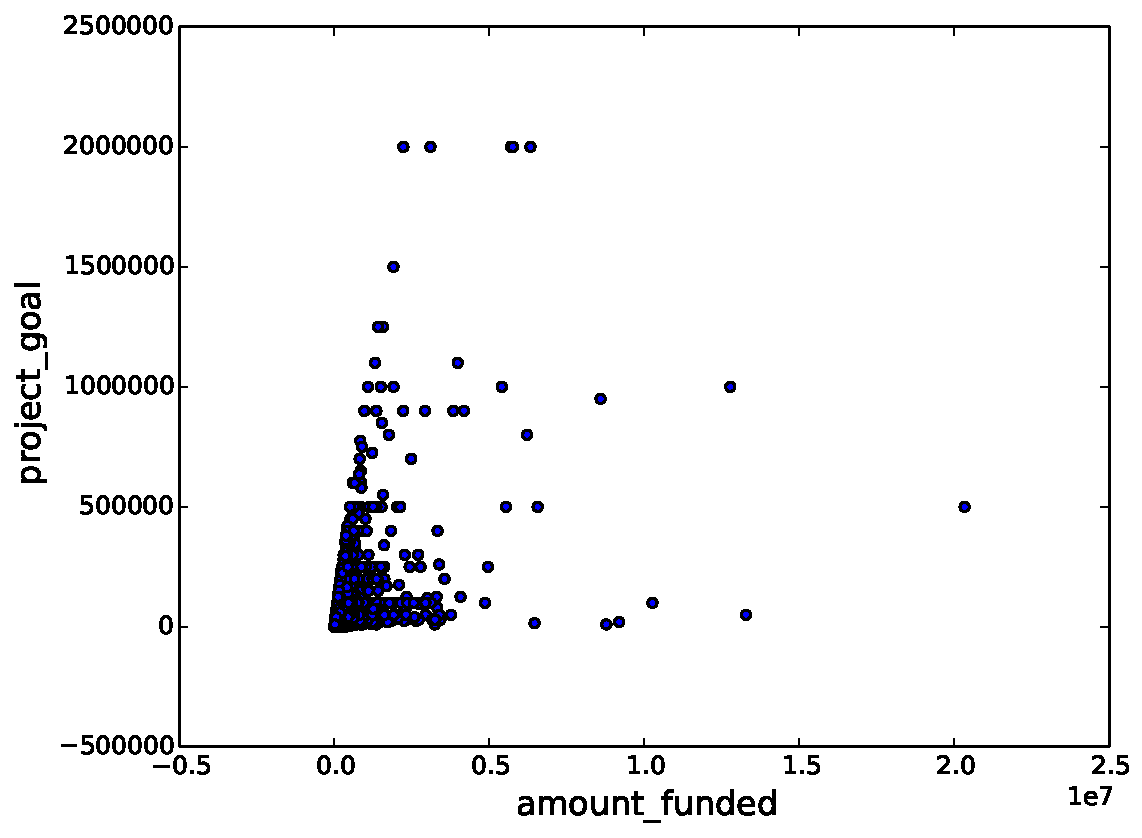
\includegraphics[width=.5\textwidth]{../Code/ClusteringPlots/amount_fundedproject_goal_scatter.pdf}\hfill
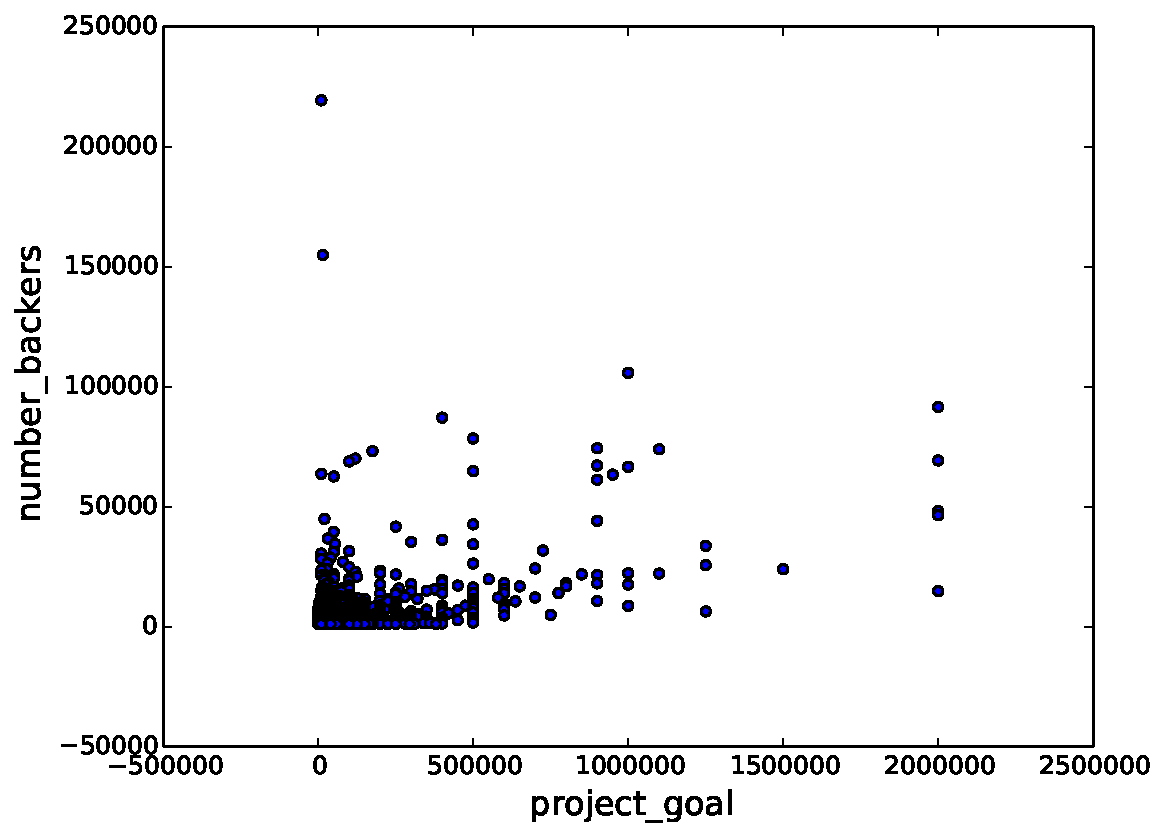
\includegraphics[width=.5\textwidth]{../Code/ClusteringPlots/project_goalnumber_backers_scatter.pdf}\hfill
\caption{Histograms and Scatter plots for all \textbf{numeric} attributes}
\label{fig:hists}
\end{figure}





\item \textbf{K-Means} is one of the most \textbf{efficient} clustering algorithms. Since this algorithm relies on a distance metric it is is also very simple and hence intuitive to understand. A possible drawback of K-Means is that it only  works well for \textbf{globular clusters} and that it is  \textbf{sensitive to outliers}. \\

\textbf{DB-Scan} is another very popular clustering algorithm that belongs in the family of \textbf{density based} methods and performs well in many settings. The basic idea behind this method is that clusters are a set of density connected instances. \textbf{In contrast to K-Means}, when using DB-Scan the number of clusters is not fixed and we can naturally handle clusters of \textbf{any shapes and sizes}. Nevertheless, DB-Scan struggles with spareness of data and in many cases does not cluster all the data (i.e. noise instances). Moreover, one of the most important drawbacks of this method is that it is \textbf{inefficient} with large data. \\

\textbf{Hierarchical clustering} is a clustering method that functions on the idea that clusters can be represented as a hierarchy. More precisely, clusters can be \textbf{merged} (Agglomerative clustering) or \textbf{split} while attempting to minimize a loss function. One of the biggest advantages of this method is that it is \textbf{easy to interpret} and choose a level of resolution for the problem. Nevertheless, the drawback of this method is that it is very \textbf{slow} when we consider a large amount of data. \\

Finally, \textbf{Mixture Models (EM)} model clusters using statistical distributions, where each multivariate distribution corresponds to a cluster. This method can find \textbf{non-globular} clusters (i.e. ellipses) and it is \textbf{easy to add domain knowledge} by changing the parameters of the distributions. Nevertheless, this clustering method is \textbf{inefficient} and faces trouble with \textbf{noise and outliers}. Also, it struggles in accurately describing \textbf{small} clusters.

\item  In order to find the best performing clustering algorithm, given our dataset, we experiment with various clustering models and values of the parameters and report the models for which we obtained the \textbf{highest silhouette score}. More precisely, the clustering methods that we explore are \textbf{K-Means, DB-Scan, Agglomerative Hierarchical clustering} and \textbf{Gaussian Mixture Models} and we vary the number of clusters from $0$ to $15$.  We also produce plots by mapping high dimensional data into $2D$ data using \emph{T-SNE}. \\

After finding the algorithm (along with the parameters) that performs the best, we extract the corresponding clusters and attempt to interpret the results. Ideally, we would have human evaluators (domain experts) to assess the results of our clustering, but this is infeasible in the context of this project.


\item 

\begin{enumerate}
\item The first method that we explore is \emph{K-Means}.

\begin{figure}[htp!]
  \begin{center}
  	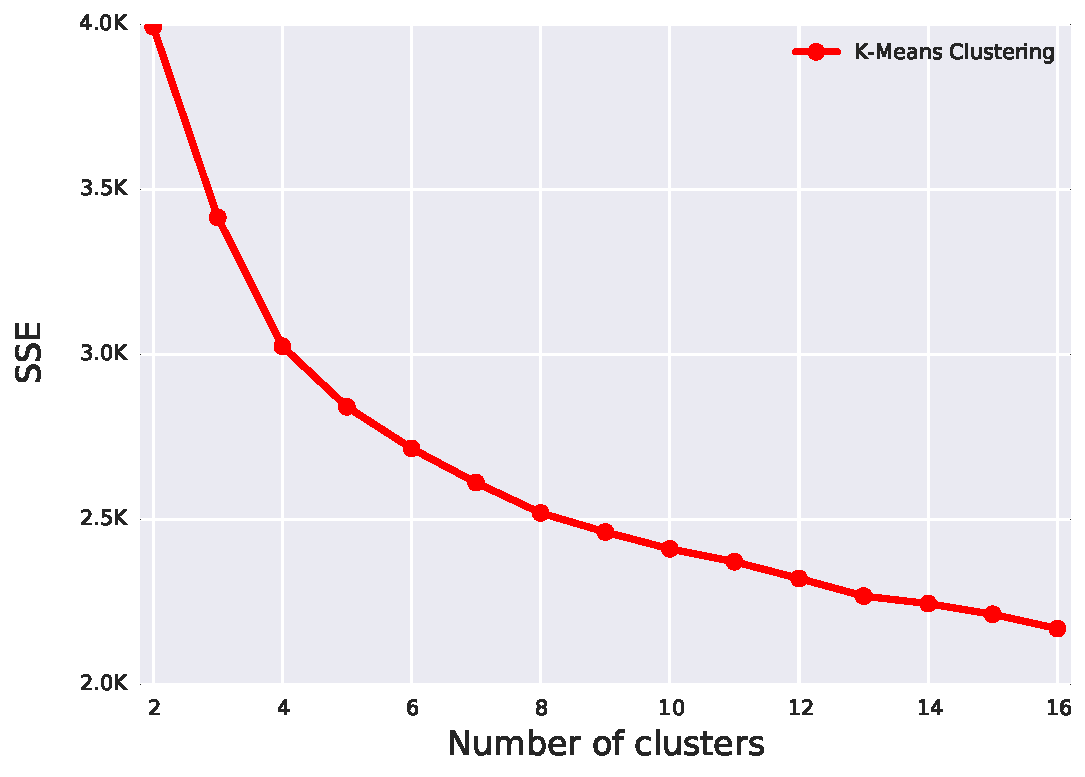
\includegraphics[width=0.6 \textwidth]{../Code/ClusteringPlots/kmeans.pdf}
  \end{center}
  \vspace{-.2cm}
  \caption{Sum of squared errors as we vary the number of clusters in the K-Means algorithm.}
  \label{fig:kmeans_elbow}
  \vspace{-.1cm}
\end{figure}

Using the ``elbow method'' we speculate that a useful clustering occurs for a number of clusters between $2$ and $6$ (Fig. \ref{fig:kmeans_elbow}). In order to assess our model we compute the \emph{silhouette} score for all the values of $k=1,2, \dots ,15$ and report the top $4$ models in terms of silhouette score.\\

\begin{figure}[htp!]
  \begin{center}
  	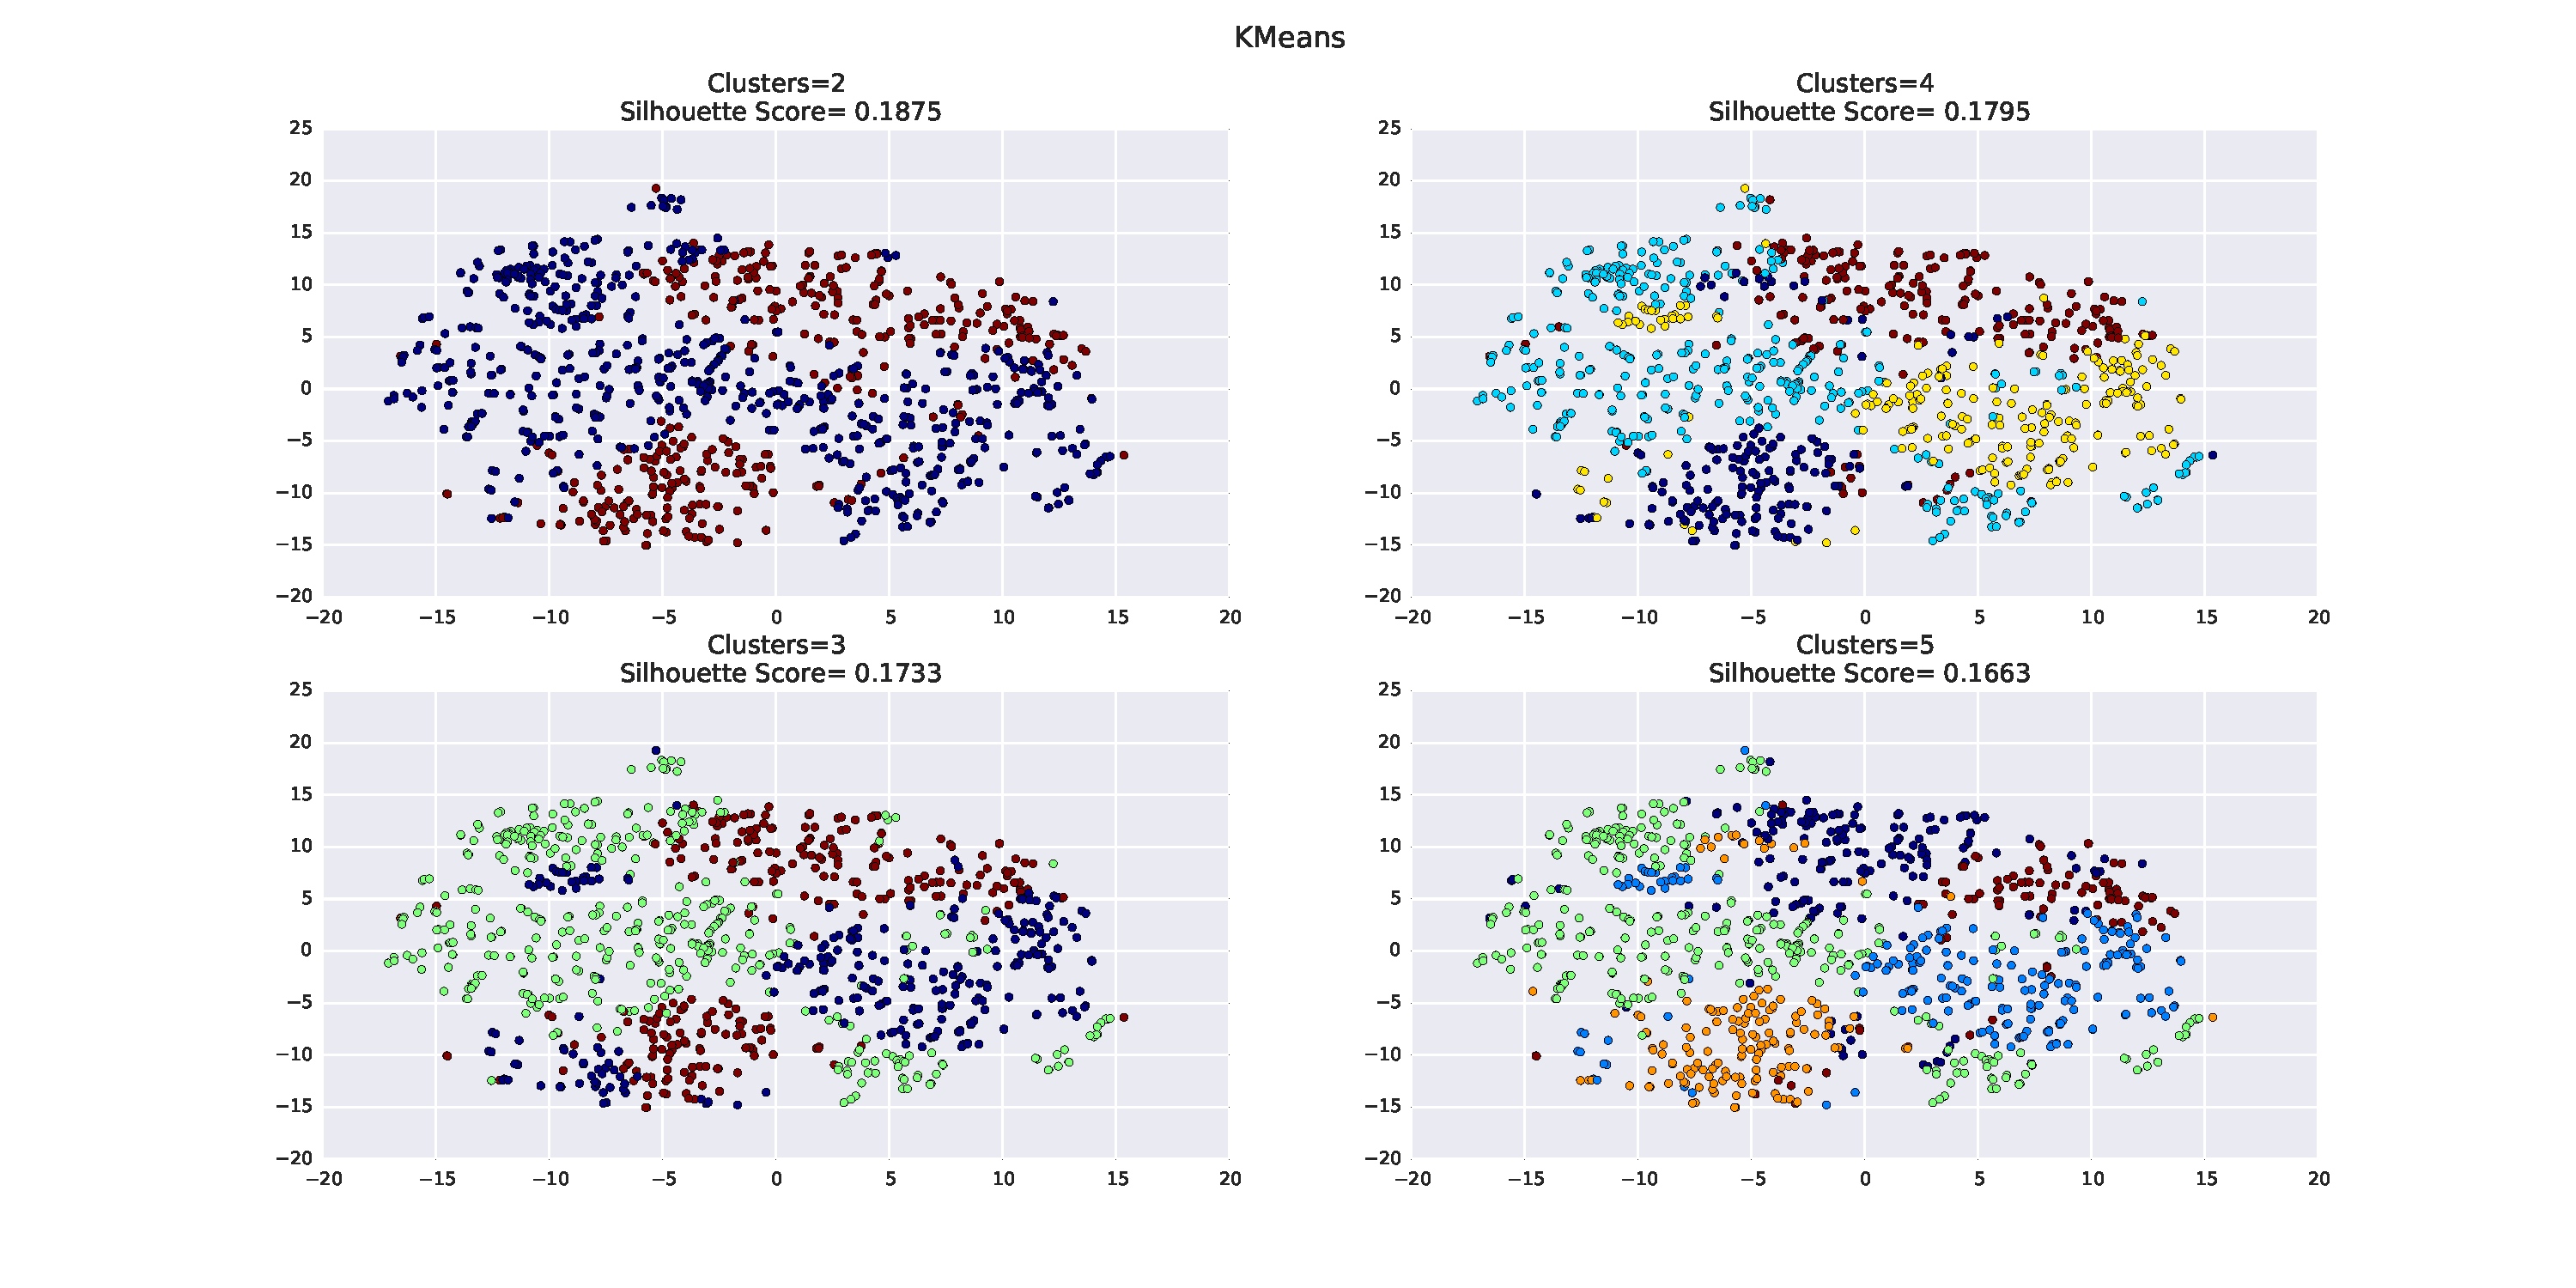
\includegraphics[width=1\textwidth]{../Code/ClusteringPlots/best_kmeans.pdf}
  \end{center}
  \vspace{-.2cm}
  \caption{Four best K-Means models as we vary $1 \leq k \leq 15$.}
  \label{fig:kmeans_best}
  \vspace{-.1cm}
\end{figure}

As we see from Figure \ref{fig:kmeans_best}, the best silhouette score is achieved for $k=2$ and is approximately equal to $0.1875$. Nevertheless, this silhouette score is still not very close to $1$, therefore, as we see next, K-Means is not the best performing clustering algorithm.


\item The second clustering algorithm that we explore is \emph{Hierarchical Agglomerative Clustering}. In this type of clustering we are given more ``freedom'' than K-Means, in the sense that we can also choose the \emph{linkage} type. More precisely, for Agglomerative Clustering the cost function (linkage) is the distance between clusters. In this project we experiment with all three common linkage methods, namely:
	\begin{itemize}
		\item Single Linkage: The distance between two clusters is the \emph{minimum} distance of their respective points 
		\item Complete Linkage: The distance between two clusters is the \emph{maximum} distance of their respective points 
		\item Average Linkage: The distance between two clusters is the \emph{average} distance of their respective points 
	\end{itemize}

More precisely, for each linkage type we vary the number of clusters $k$ such that $k=1,2 \dots, 15$ \textbf{but only report the four values of $k$ for which we calculated the largest silhouette score.} \\

\begin{figure}[htp!]
  \begin{center}
  	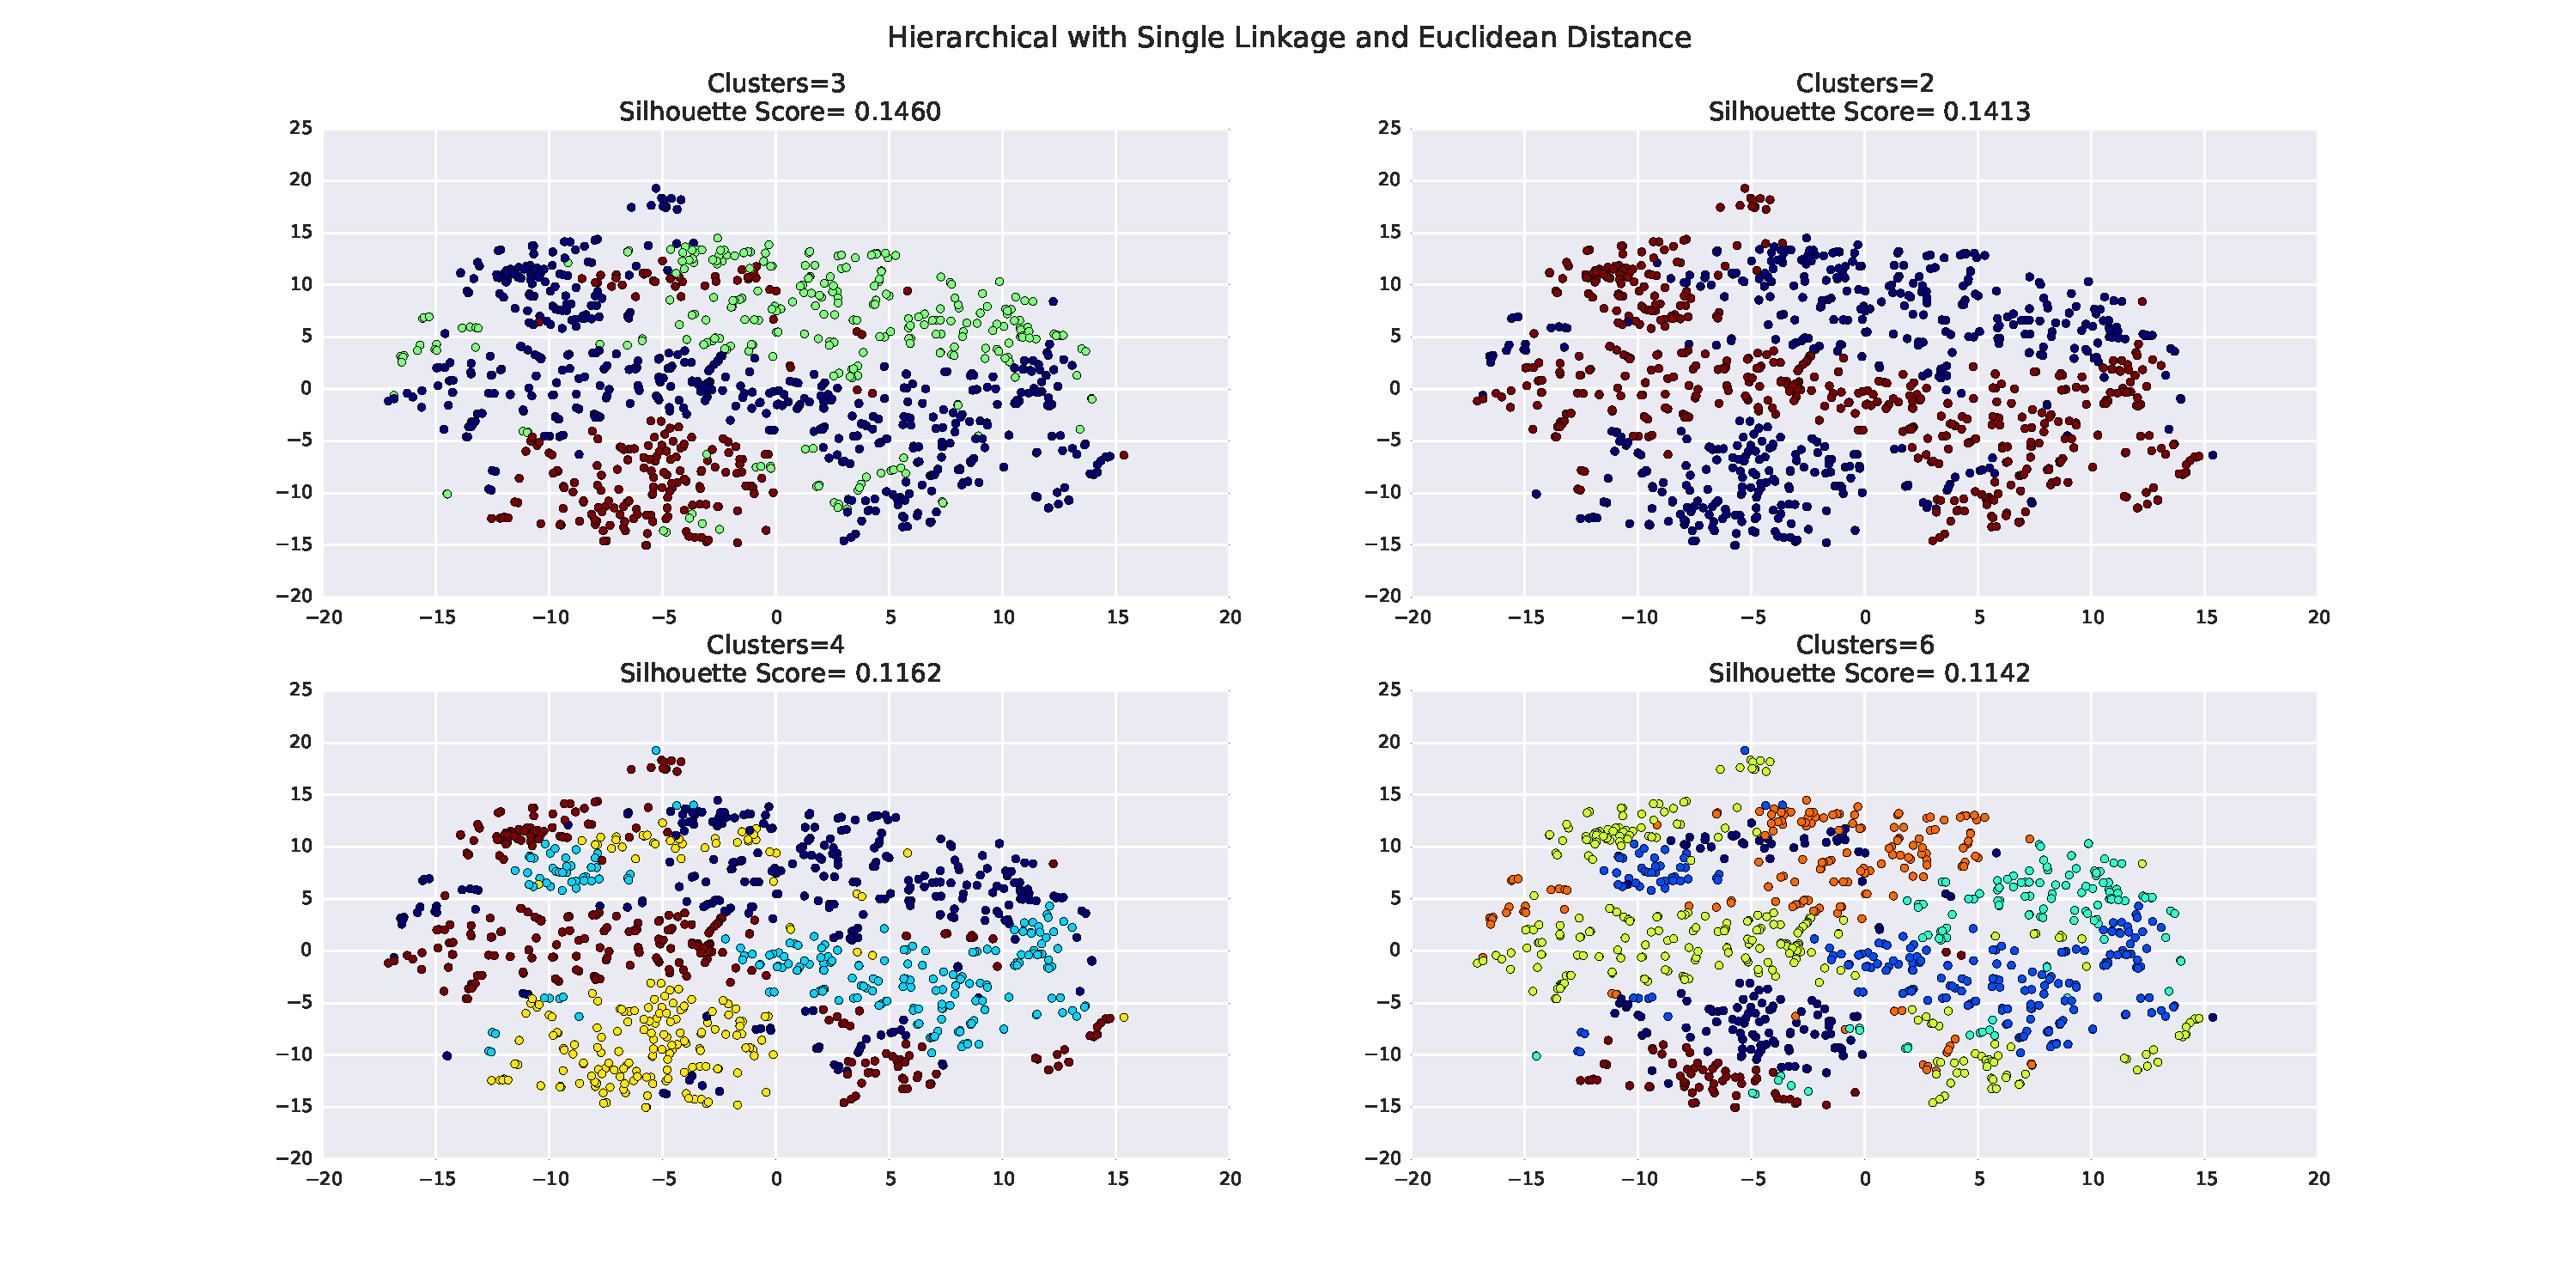
\includegraphics[width=1\textwidth]{../Code/ClusteringPlots/single_link}
  \end{center}
  \vspace{-.2cm}
  \caption{Four best Single Linkage models as we vary $1 \leq k \leq 40$.}
  \label{fig:single_link}
  \vspace{-.1cm}
\end{figure}

\begin{figure}[htp!]
  \begin{center}
  	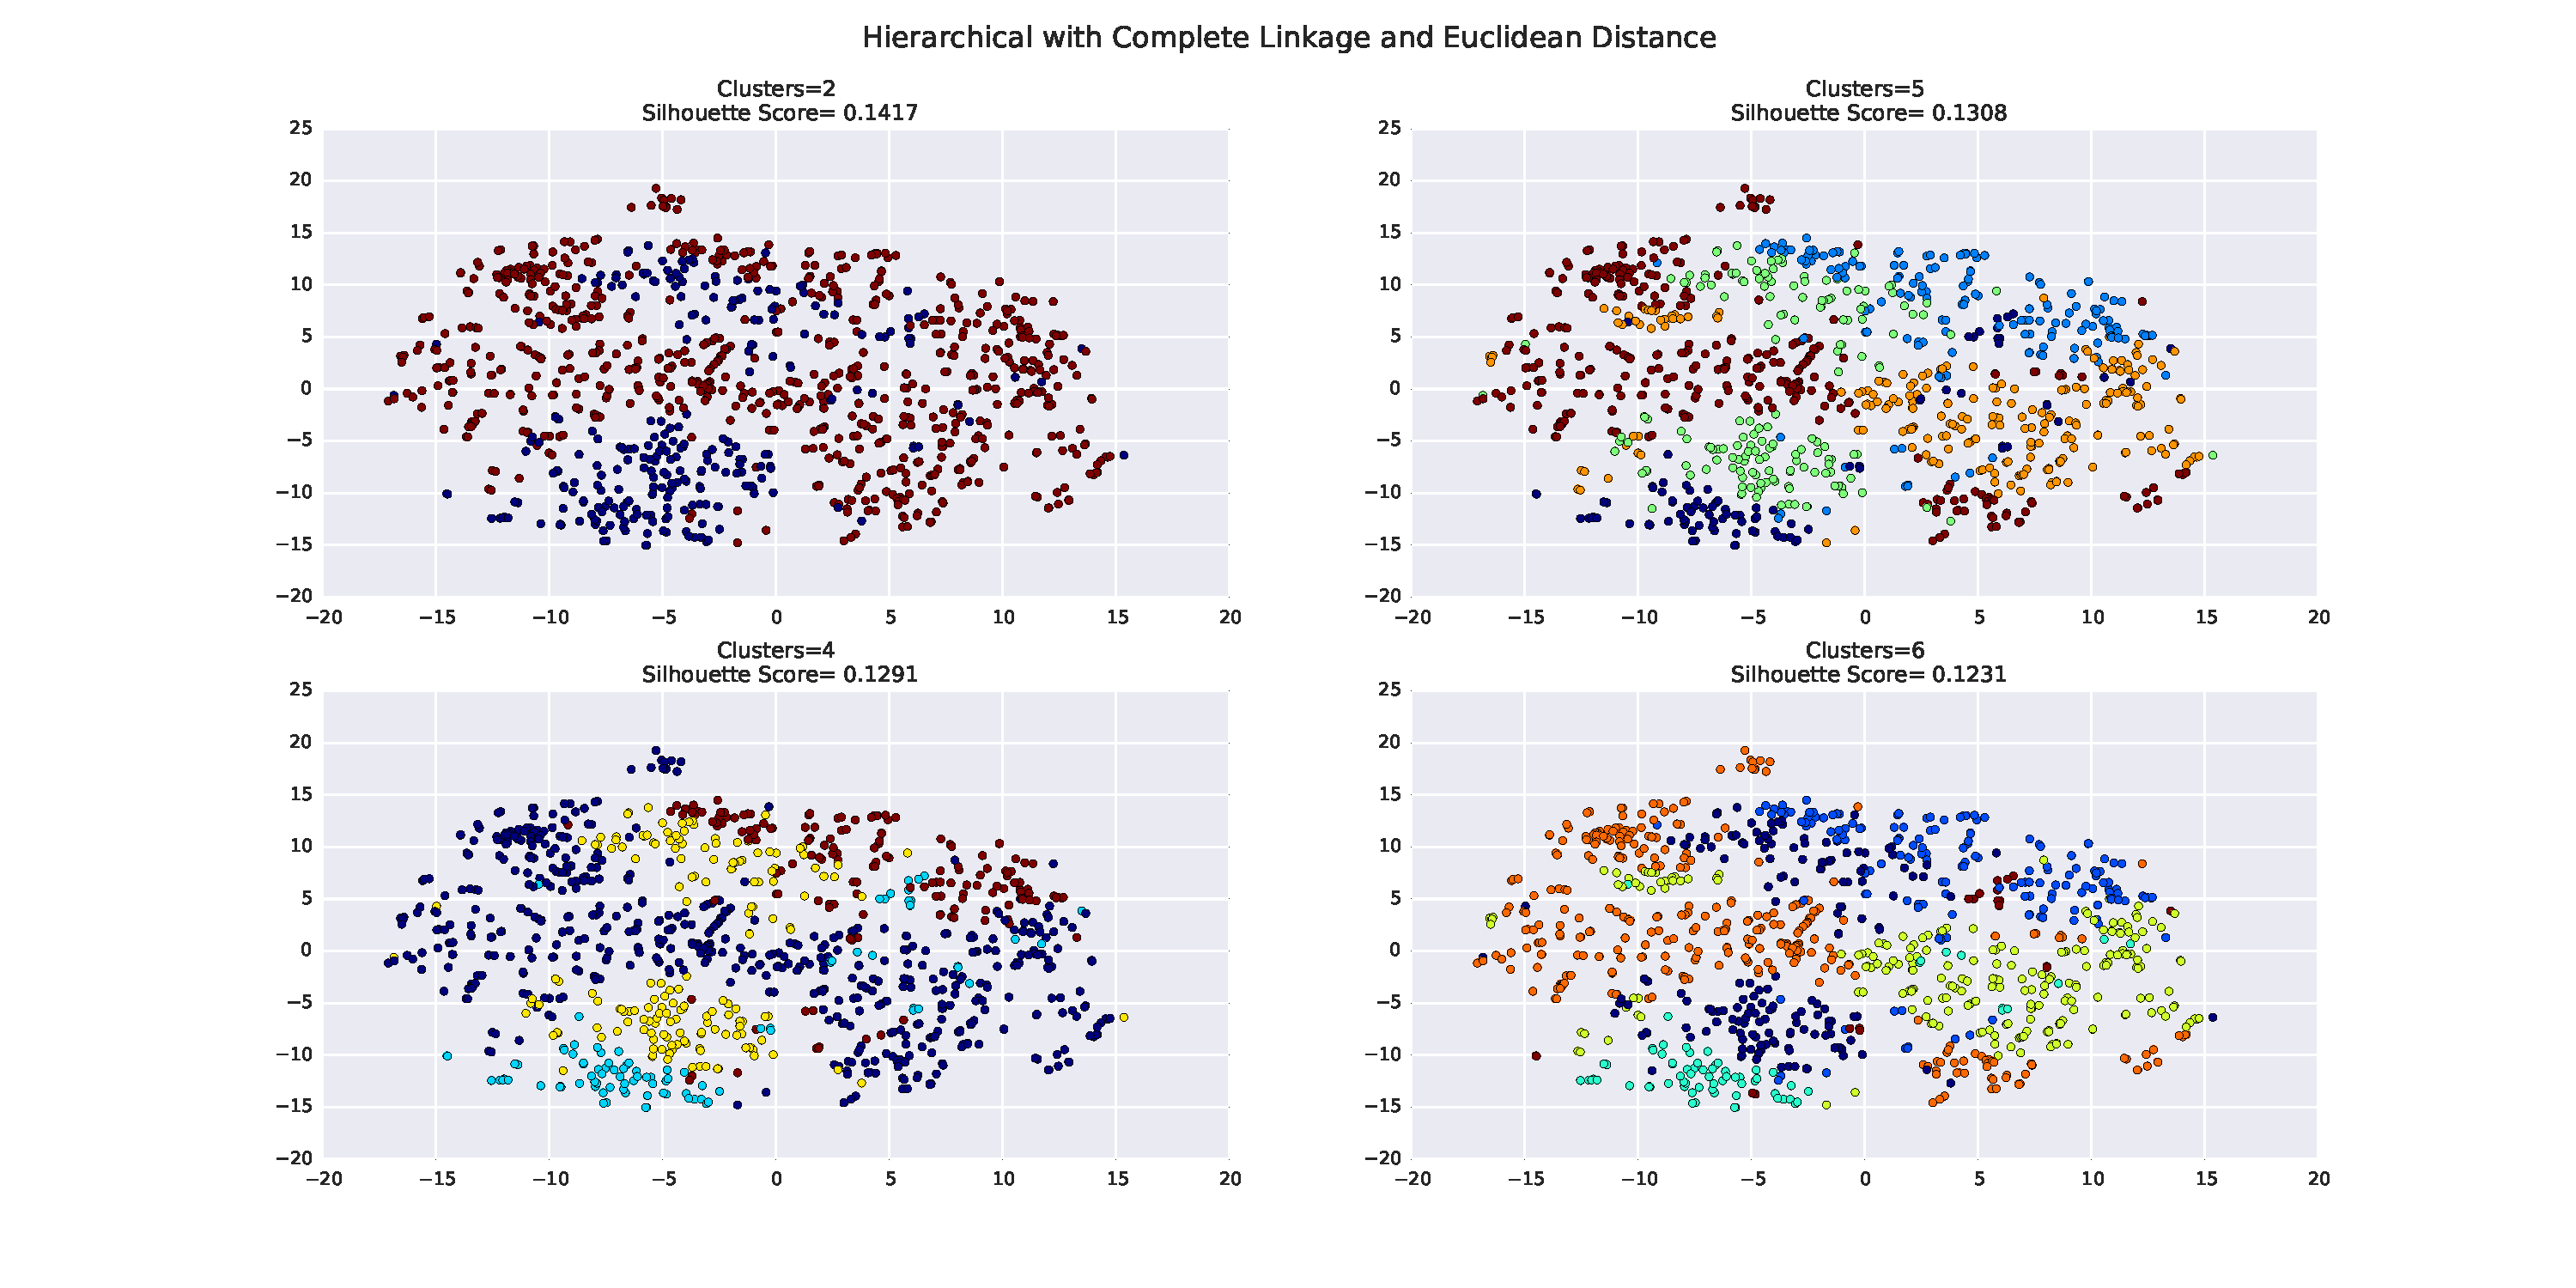
\includegraphics[width=1\textwidth]{../Code/ClusteringPlots/complete_link}
  \end{center}
  \vspace{-.2cm}
  \caption{Four best Single Linkage models as we vary $1 \leq k \leq 40$.}
  \label{fig:complete_link}
  \vspace{-.1cm}
\end{figure}


\begin{figure}[htp!]
  \begin{center}
  	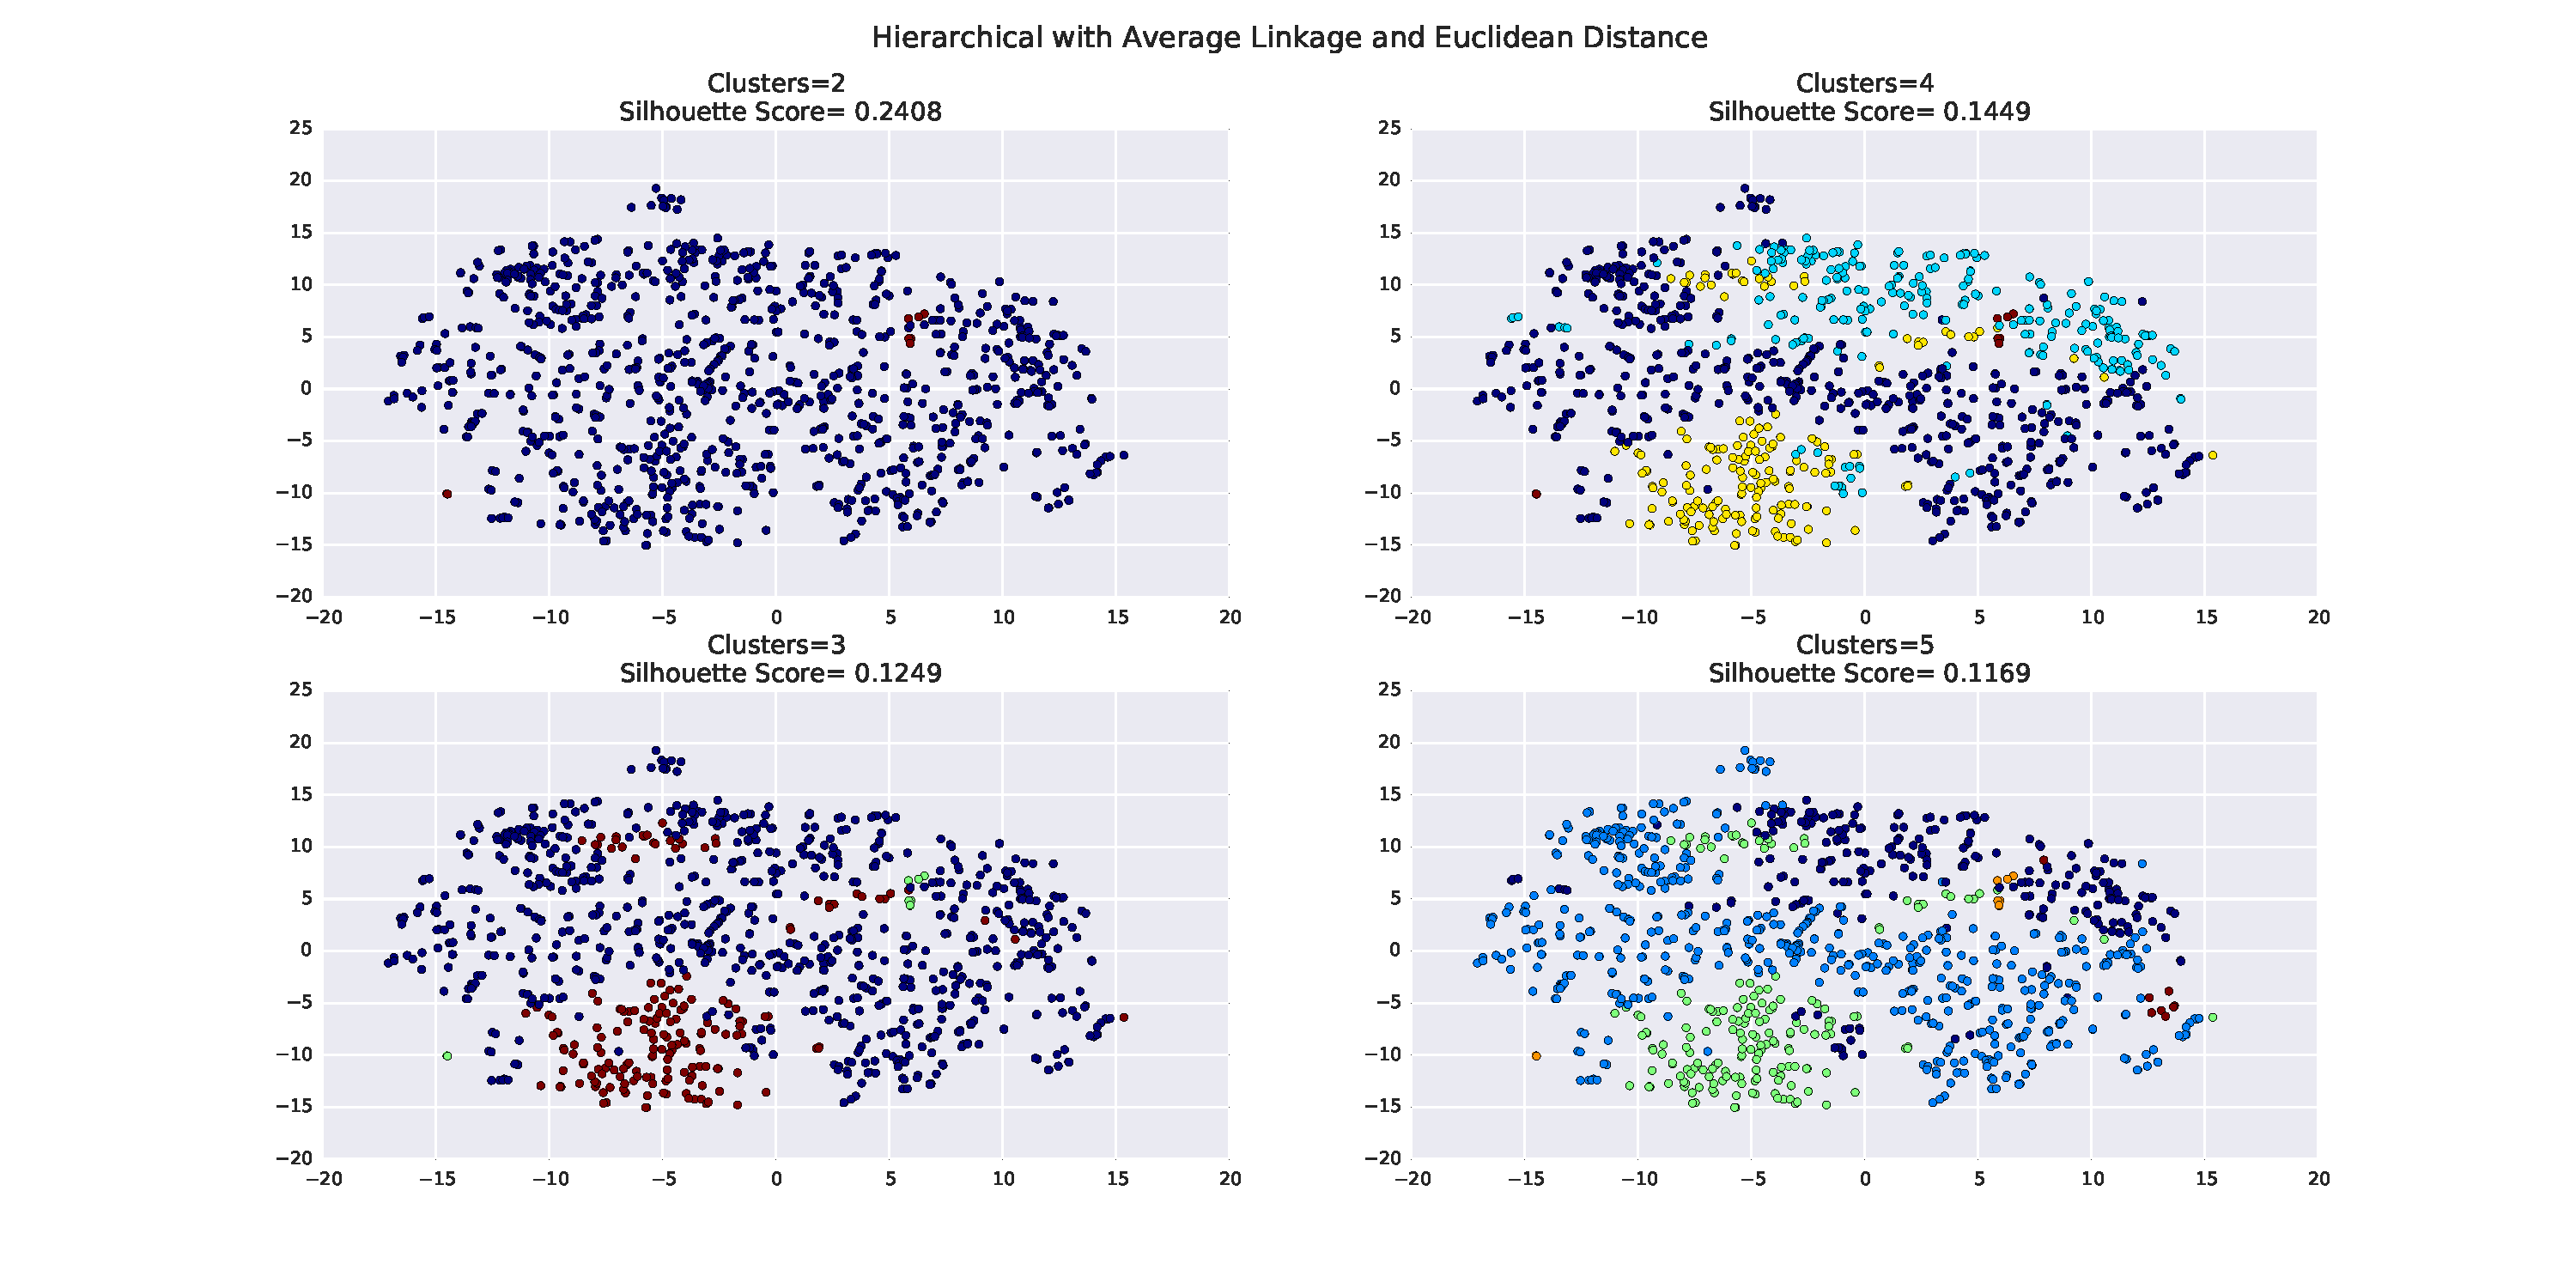
\includegraphics[width=1\textwidth]{../Code/ClusteringPlots/average_link}
  \end{center}
  \vspace{-.2cm}
  \caption{Four best Single Linkage models as we vary $1 \leq k \leq 40$.}
  \label{fig:average_link}
  \vspace{-.1cm}
\end{figure}

As we see from Figures \ref{fig:single_link}, \ref{fig:complete_link}, \ref{fig:average_link}, single and complete linkage perform poorly achieving a silhouette score of $0.1460$ and $0.1417$, respectively. Average linkage performs the best out of the three methods, achieving a score of $0.2408$ for $k=2$. \\

Also, in Figure \ref{fig:dendro} we see the that if we let the euclidean distance be greater than $29$ we get two clusters.

\begin{figure}[htp!]
  \begin{center}
  	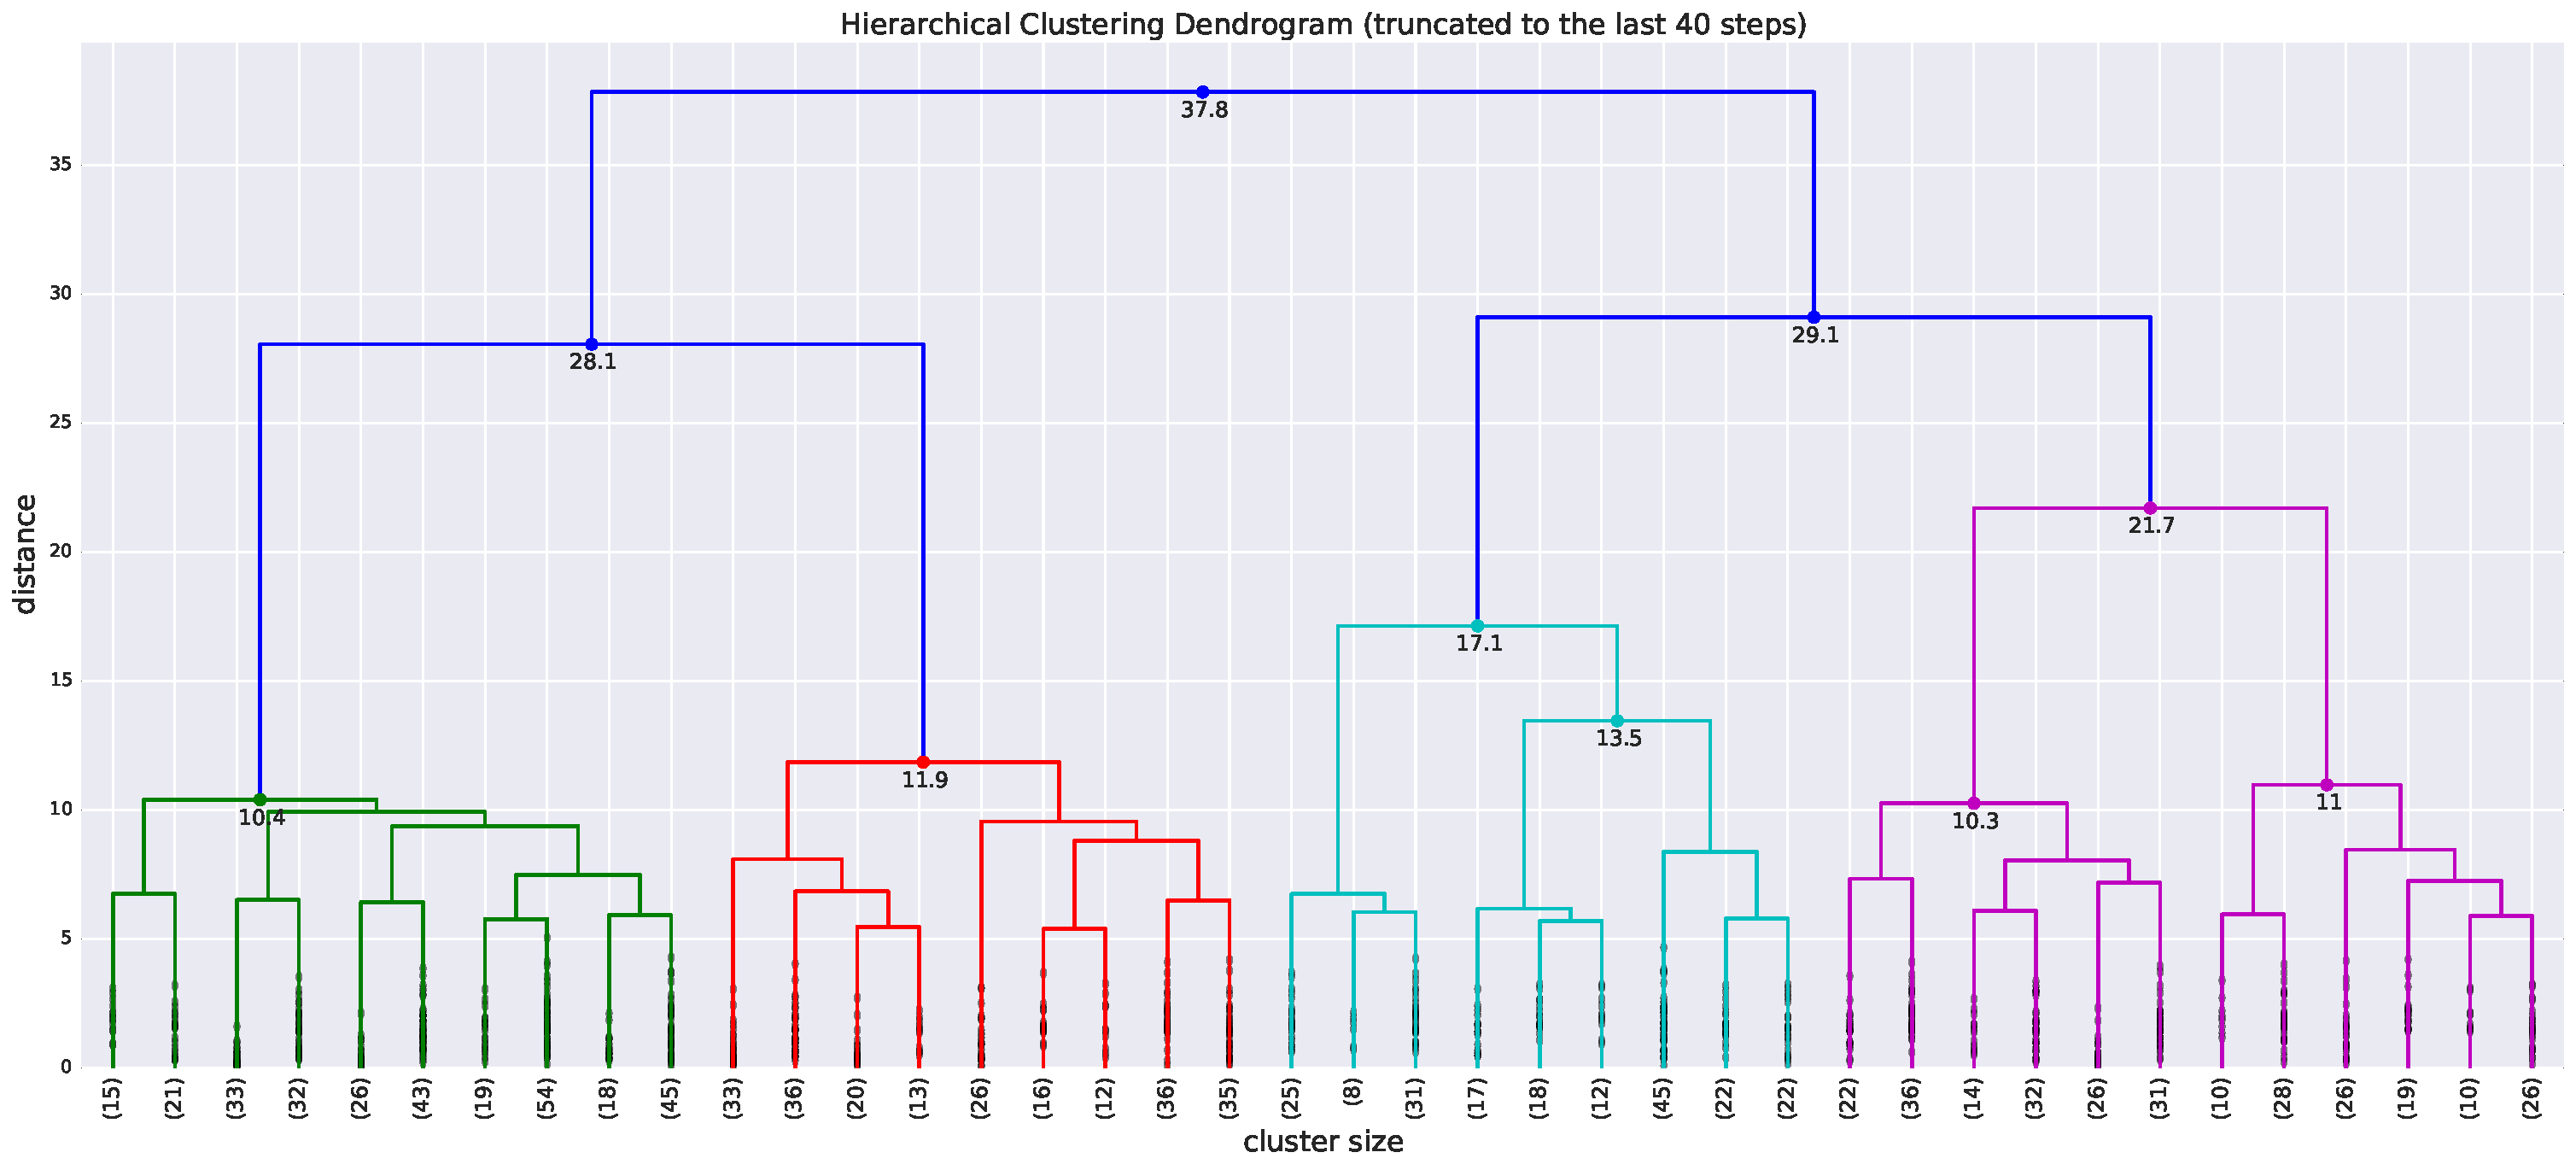
\includegraphics[width=1\textwidth]{../Code/ClusteringPlots/dendro}
  \end{center}
  \vspace{-.2cm}
  \caption{Dendrogram for Average Linkage}
  \label{fig:dendro}
  \vspace{-.1cm}
\end{figure}

\item The next clustering method that we explore, is \emph{DB-Scan}. In contrast to the previously seen clustering algorithms, in this case we do not need to supply the number of clusters, as the algorithm finds the number of clusters based on $\epsilon$ and $MinPoints$. Heuristically, we found that letting $MinPoints > 4$ always resulted in the same clustering where only one cluster was present. Therefore, we vary $1 \leq MinPoints \leq 4$ and we let $\epsilon=0.1+ 0.1t$ for $t=0, 1, \dots ,34$. As we varied $MinPoints$ between $1$ and $5$ we observed no significant changes in the value of the silhouette score. Nevertheless, the value of $\epsilon$ played a crucial role in getting a good clustering model. In fact, by looking at Figure \ref{fig:best_dbscan} we see that we achieve the highest silhouette score for $k=2$ and $0.1 \leq \epsilon \leq 0.4$.
\begin{figure}[htp!]
  \begin{center}
  	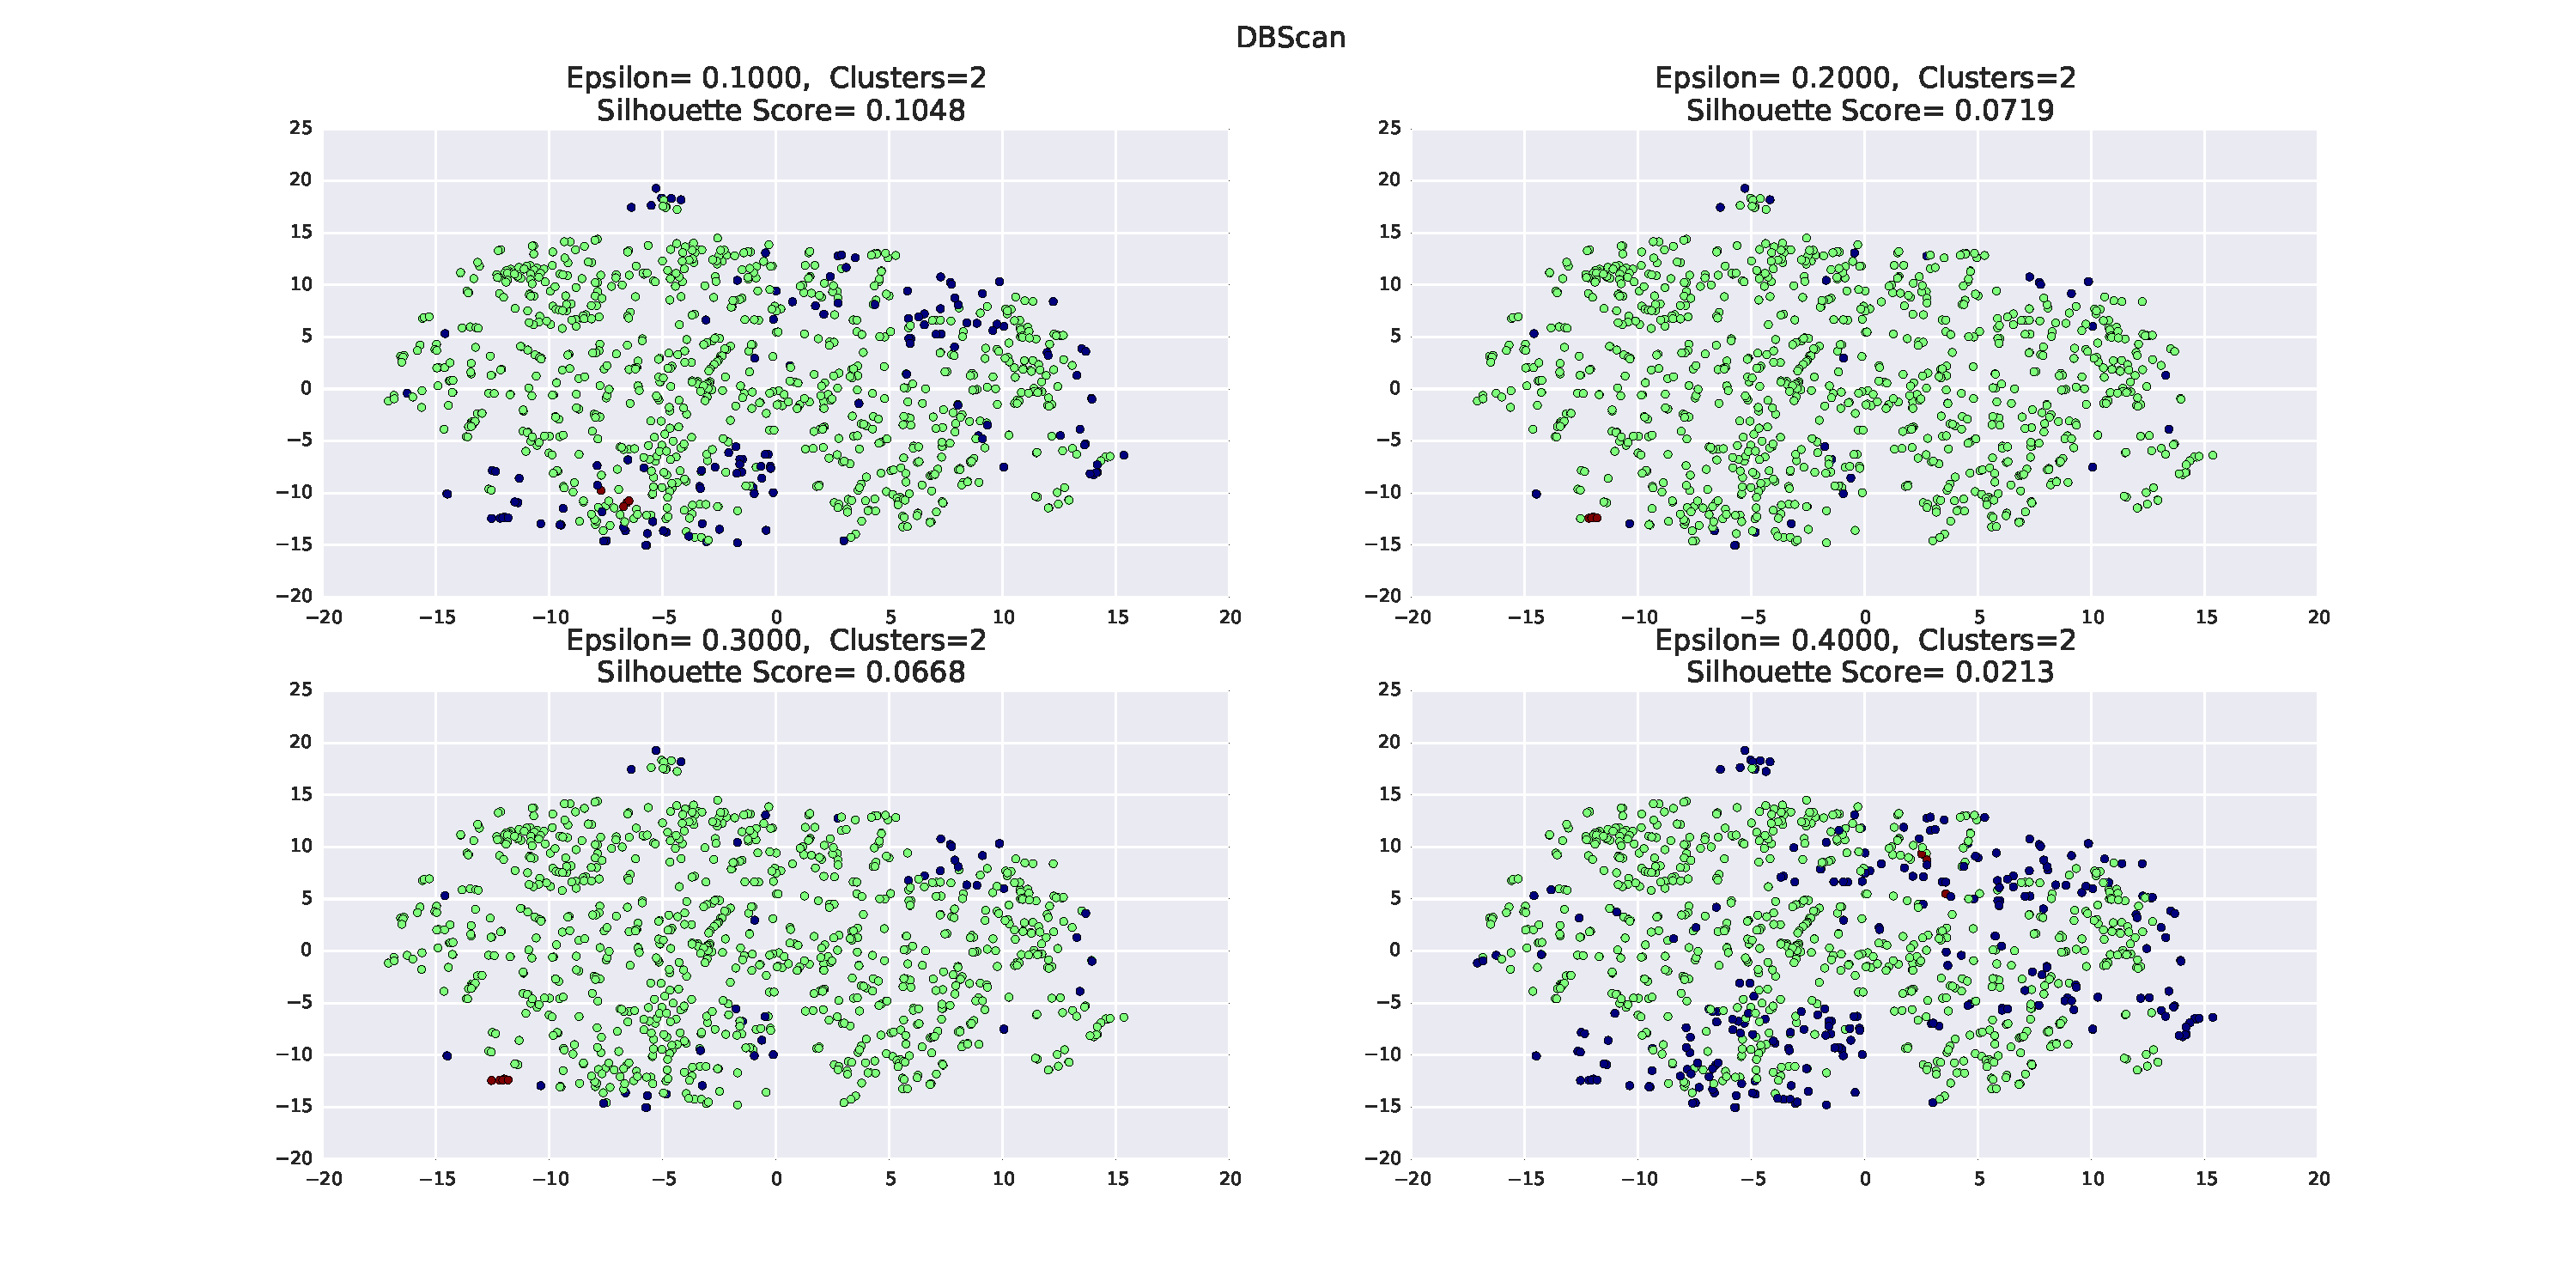
\includegraphics[width=1\textwidth]{../Code/ClusteringPlots/best_dbscan_minpoints_5}
  \end{center}
  \vspace{-.2cm}
  \caption{Four best Single Linkage models as we vary $1 \leq k \leq 40$ and fix $MinPoints=4$.}
  \label{fig:best_dbscan}
  \vspace{-.1cm}
\end{figure}


\item Finally, we try the \emph{Expected Maximization} algorithm where we use Gaussian Priors. We see that this model performs very poorly compared to other clustering techniques (Fig. \ref{fig:best_gaussian}). According to this clustering model, the number of clusters that achieve the highest silhouette score ($-0.0385$) is $14$, which is very different than the number of clusters suggested by our previous analysis. 

\begin{figure}[H]
  \begin{center}
  	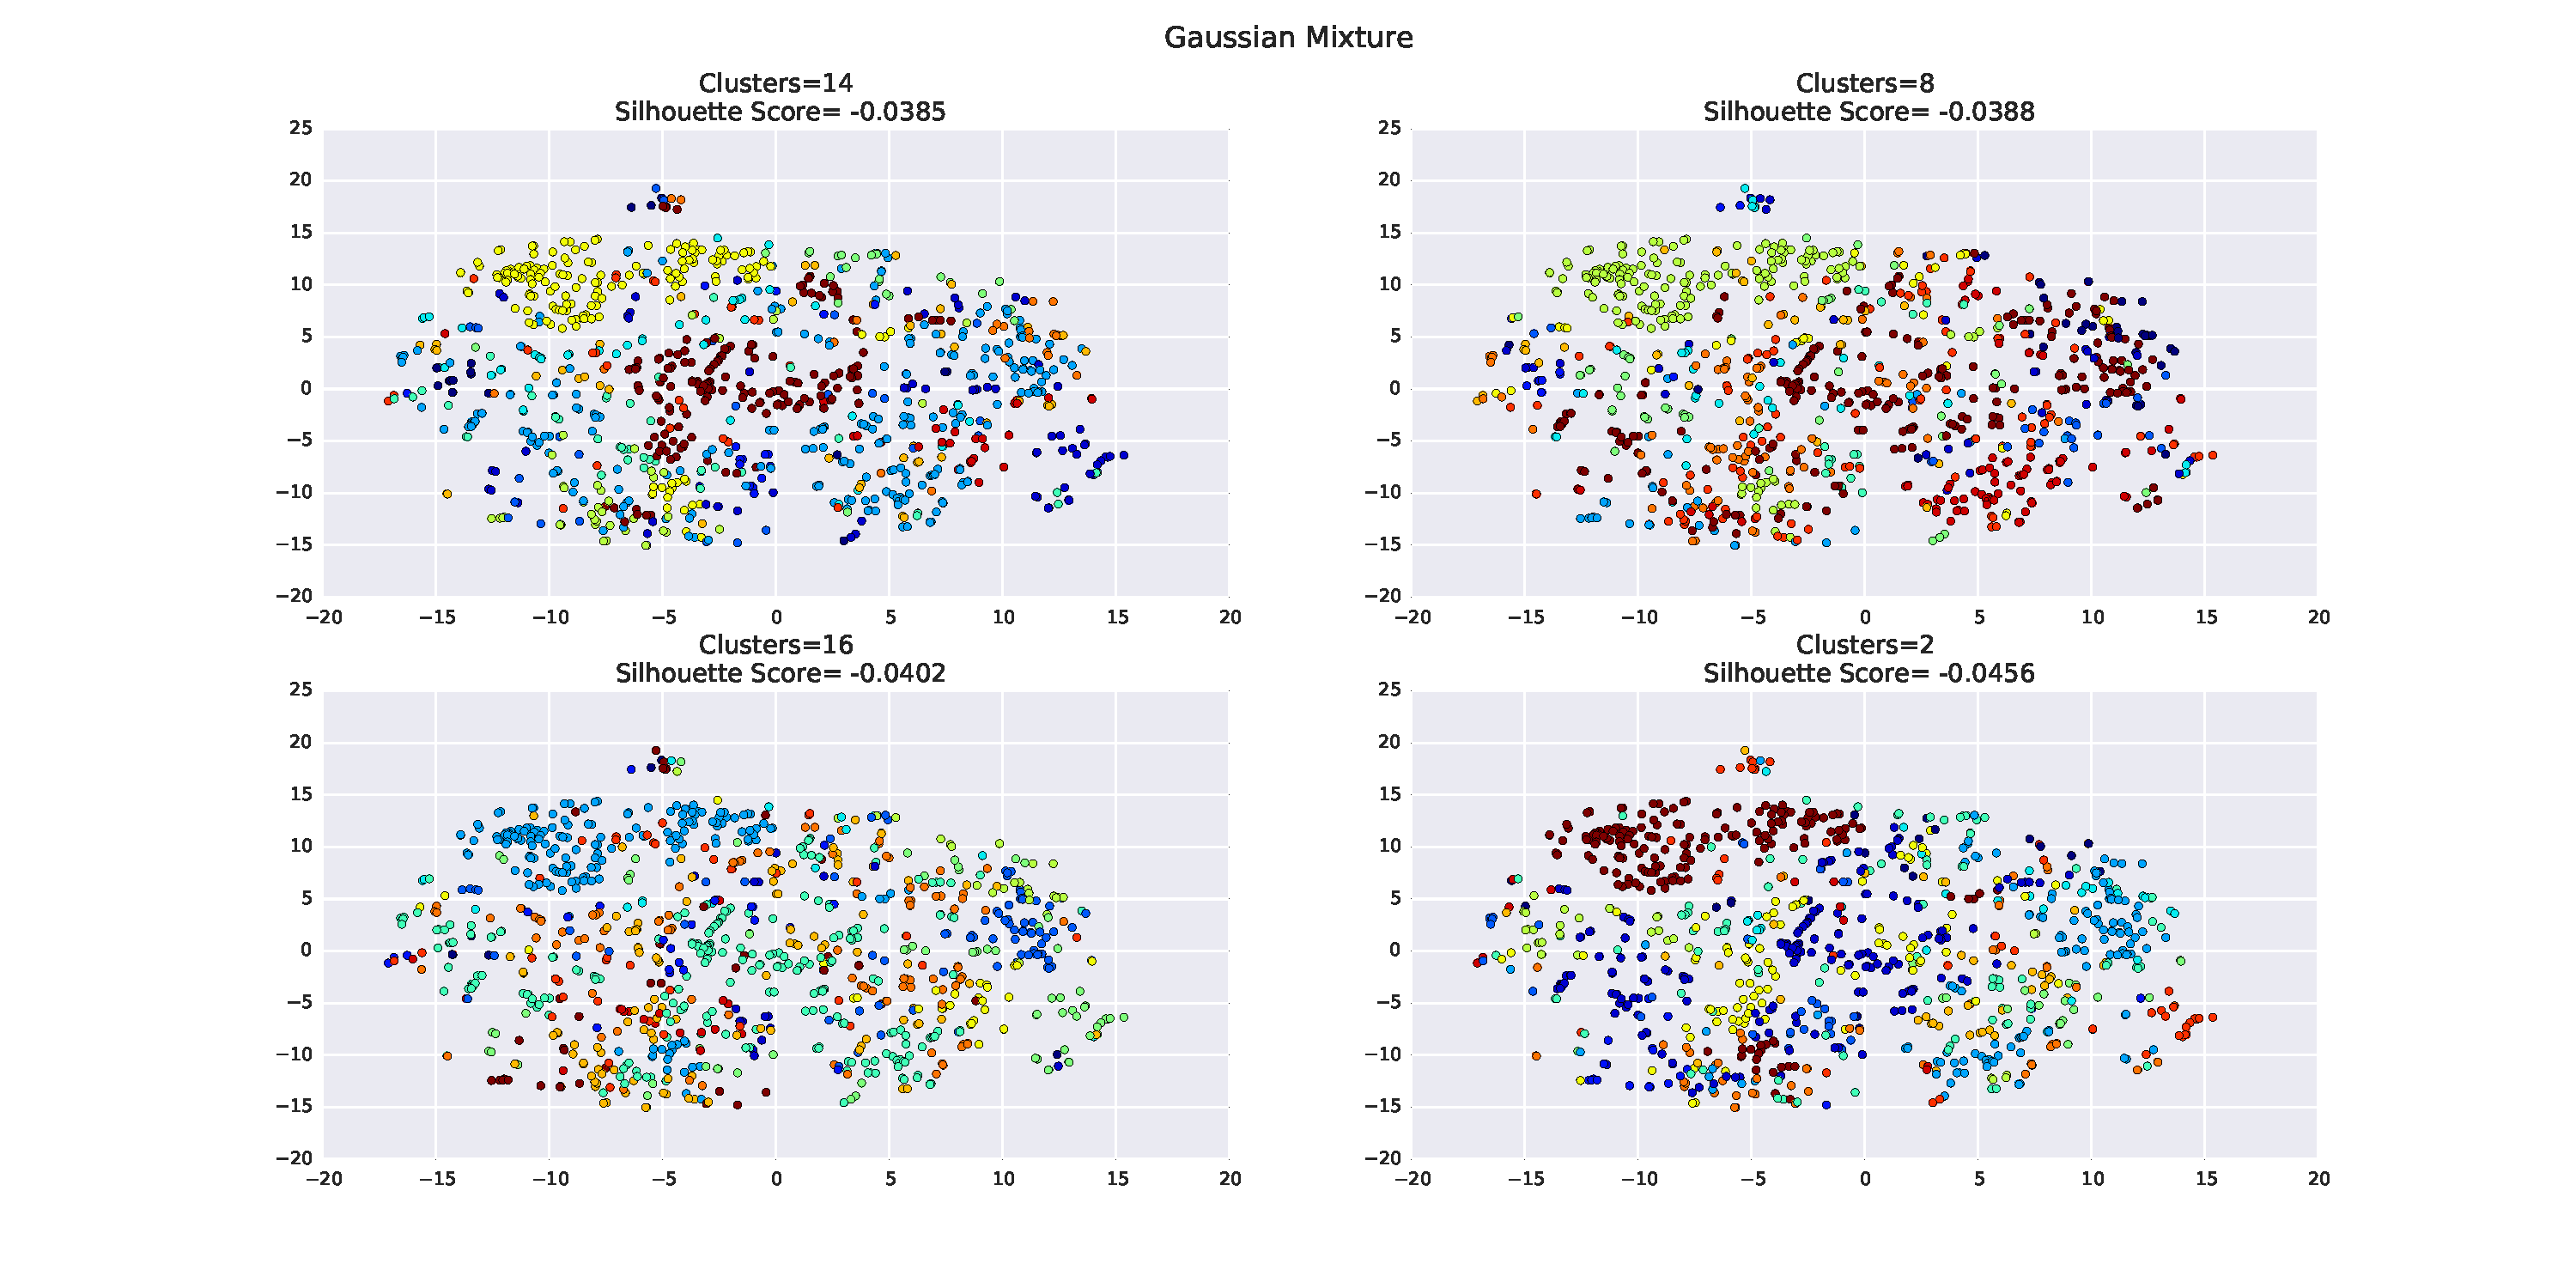
\includegraphics[width=1\textwidth]{../Code/ClusteringPlots/best_gaussian}
  \end{center}
  \vspace{-.2cm}
  \caption{Four best Gaussian Mixture models as we vary $1 \leq k \leq 15$.}
  \label{fig:best_gaussian}
  \vspace{-.1cm}
\end{figure}



\end{enumerate}

\textbf{After analyzing} various models we conclude that the best performing model is \textbf{Agglomerative Hierarchical Clustering with Average linkage and the Euclidean distance metric}. 

\item Looking further into our clustering results, we see that there exist $2$ clusters of unequal sizes. Namely, the first clusters consists of $270$ instances, whereas, the second cluster consists of $743$ instances. \\

A good candidate that the company could investigate further are the points that lie in cluster $1$. In this cluster we see that the majority of projects are in the \textbf{Video Game} category and are based in \textbf{New York}. These are good opportunities that \emph{Redwood Capital} could explore since technology investments are usually profit motivated.


 \end{enumerate} %end Q1

\end{homeworkProblem}
\clearpage
%----------------------------------------------------------------------------------------
%	PROBLEM 4
%----------------------------------------------------------------------------------------
\begin{homeworkProblem}[Problem \arabic{homeworkProblemCounter}: Brainstorming for Financial Investment Data Mining (10 points)]

The firm has asked you for new ideas about how data mining can be used to improve their investment strategy. Apply a structured brainstorming process to generate 3-5 possible ideas for using data mining to improve financial investments.\\

For each generated idea, provide a brief description of:
\begin{enumerate}
\item What type of investment problem is being addressed, e.g. identifying promising new start-up companies or determining how much money to invest in a particular company.
\item	What type of data mining task is involved: classification, prediction, cluster analysis, or association analysis.
\item	What data-sets would need to be collected for the data mining task.
\item	How could Redwood Capital use the resulting model (supervised learning) or patterns (unsupervised learning)?

\end{enumerate}


\noindent\rule{16cm}{0.9pt}
		
\large{\textbf{\underline{Answer:}}}

\begin{enumerate}
\item  \textsc{Improve Investment Strategies:}  A possible idea would be to use classification to further expand and advance the models we have explored in Problem 1, in order to classify start up companies as promising or not. In order to perform such a task more accurately, the company could enhance the existing dataset to include more instances thus covering a broader  number of cases that would allow the model to generalize with higher accuracy. \\

\item  \textsc{Stock Market Prediction:}  Another possibility where data mining could be used in this sector, is in attempting to predict the stock market behavior. This task falls under the \emph{time series analysis} approach and is certainly very complex. Nevertheless, the company could vastly benefit from a such a model since it would know the appropriate times to invest. The dataset to be used for such a task, could be the behavior of the stock market during the past decade.\\

\item  \textsc{Patterns of Successful Companies:}  Using data mining we could explore further what kind of patterns occur in successful companies. Finding these patterns would allow the company to optimize their investment strategies by looking for patterns that make start up companies successful. We could use association analysis (unsupervised learning) for this task and use a similar dataset as the one provided in Problem 1.


\end{enumerate}
\end{homeworkProblem}

\end{document}
